% ******************************* PhD Thesis Template **************************
% Please have a look at the README.md file for info on how to use the template

\documentclass[a4paper,11pt,times,numbered,print,index]{Classes/PhDThesisPSnPDF}

% ******************************************************************************
% ******************************* Class Options ********************************
% *********************** See README for more details **************************
% ******************************************************************************

% `a4paper'(The University of Cambridge PhD thesis guidelines recommends a page
% size a4 - default option) or `a5paper': A5 Paper size is also allowed as per
% the Cambridge University Engineering Deparment guidelines for PhD thesis
%
% `11pt' or `12pt'(default): Font Size 10pt is NOT recommended by the University
% guidelines
%
% `oneside' or `twoside'(default): Printing double side (twoside) or single
% side.
%
% `print': Use `print' for print version with appropriate margins and page
% layout. Leaving the options field blank will activate Online version.
%
% `index': For index at the end of the thesis
%
% `draft': For draft mode without loading any images (same as draft in book)
%
% `draftmode': Special draft mode with line numbers, images, and water mark with
% timestamp and custom text. Position of the text can also be modified.
%
% `abstract': To generate only the title page and abstract page with
% dissertation title and name, to submit to the Student Registry
%
% `chapter`: This option enables only the specified chapter and it's references
%  Useful for review and corrections.
%
% ************************* Custom Page Margins ********************************
%
% `custommargin`: Use `custommargin' in options to activate custom page margins,
% which can be defined in the preamble.tex. Custom margin will override
% print/online margin setup.
%
% *********************** Choosing the Fonts in Class Options ******************
%
% `times' : Times font with math support. (The Cambridge University guidelines
% recommend using times)
%
% `fourier': Utopia Font with Fourier Math font (Font has to be installed)
%            It's a free font.
%
% `customfont': Use `customfont' option in the document class and load the
% package in the preamble.tex
%
% default or leave empty: `Latin Modern' font will be loaded.
%
% ********************** Choosing the Bibliography style ***********************
%
% `authoryear': For author-year citation eg., Krishna (2013)
%
% `numbered': (Default Option) For numbered and sorted citation e.g., [1,5,2]
%
% `custombib': Define your own bibliography style in the `preamble.tex' file.
%              `\RequirePackage[square, sort, numbers, authoryear]{natbib}'.
%              This can be also used to load biblatex instead of natbib
%              (See Preamble)
%
% **************************** Choosing the Page Style *************************
%
% `default (leave empty)': For Page Numbers in Header (Left Even, Right Odd) and
% Chapter Name in Header (Right Even) and Section Name (Left Odd). Blank Footer.
%
% `PageStyleI': Chapter Name next & Page Number on Even Side (Left Even).
% Section Name & Page Number in Header on Odd Side (Right Odd). Footer is empty.
%
% `PageStyleII': Chapter Name on Even Side (Left Even) in Header. Section Number
% and Section Name in Header on Odd Side (Right Odd). Page numbering in footer


% ********************************** Preamble **********************************
% Preamble: Contains packages and user-defined commands and settings
% ******************************************************************************
% ****************************** Custom Margin *********************************

% Add `custommargin' in the document class options to use this section
% Set {innerside margin / outerside margin / topmargin / bottom margin}  and
% other page dimensions
\ifsetCustomMargin
  \RequirePackage[left=37mm,right=30mm,top=35mm,bottom=30mm]{geometry}
  \setFancyHdr % To apply fancy header after geometry package is loaded
\fi

% *****************************************************************************
% ******************* Fonts (like different typewriter fonts etc.)*************

% Add `customfont' in the document class option to use this section

\ifsetCustomFont
  % Set your custom font here and use `customfont' in options. Leave empty to
  % load computer modern font (default LaTeX font).
  \RequirePackage{helvet}
\fi

% *****************************************************************************
% **************************** Custom Packages ********************************

% ************************* Algorithms and Pseudocode **************************

%\usepackage{algpseudocode}


% ********************Captions and Hyperreferencing / URL **********************

% Captions: This makes captions of figures use a boldfaced small font.
%\RequirePackage[small,bf]{caption}

\RequirePackage[labelsep=space,tableposition=top]{caption}
\renewcommand{\figurename}{Fig.} %to support older versions of captions.sty


% *************************** Graphics and figures *****************************

%\usepackage{rotating}
%\usepackage{wrapfig}

% Uncomment the following two lines to force Latex to place the figure.
% Use [H] when including graphics. Note 'H' instead of 'h'
%\usepackage{float}
%\restylefloat{figure}

% Subcaption package is also available in the sty folder you can use that by
% uncommenting the following line
% This is for people stuck with older versions of texlive
%\usepackage{sty/caption/subcaption}
%\usepackage{subcaption}

% ********************************** Tables ************************************
\usepackage{booktabs} % For professional looking tables
\usepackage{multirow}
\usepackage{fancybox}
\usepackage{soul}

%\usepackage{multicol}
%\usepackage{longtable}
%\usepackage{tabularx}


% ***************************** Math and SI Units ******************************

\usepackage{amsfonts}
\usepackage{amsmath}
\usepackage{amssymb}
\usepackage{siunitx} % use this package module for SI units

\usepackage{hyperref}

\usepackage{algorithm}
\usepackage[noend]{algpseudocode}



\usepackage{subfig}

\usepackage{balance}
\usepackage{longtable}
%
\newtheorem{thm}{Theorem}
\newtheorem{corr}{Corollary}
\newtheorem{lemma}{Lemma}
\newtheorem{pty}{Property}
\usepackage{array}

\newcommand{\addpic}{\includegraphics[width=10em height=10em]{example-image}}
\newcolumntype{C}{>{\centering\arraybackslash}m{12em}}

\newcommand{\red}[1]{\textcolor{red}{#1}}
\newcommand{\note}[1]{\red{#1}}

\newcommand*{\thead}[1]{\multicolumn{1}{c}{\bfseries #1}}



\newtheorem{definition}{}
% https://tex.stackexchange.com/questions/17619/common-per-section-numbering-of-theorems-lemmas-etc
%\newtheorem{lemma}[definition]{Lemma}
\newtheorem{proof}{Proof}
\newtheorem{corollary}[definition]{Corollary}
\newtheorem{theorem}[definition]{Theorem}
\newtheorem{example}[definition]{Example}
\newtheorem{remark}{Remark}
\newtheorem{question}{Question}


\hyphenpenalty 10000
\exhyphenpenalty 10000
%Numbers

% ******************************* Line Spacing *********************************

% *********************Custom commands ******************************%

%%% Commands
%\newcommand{\one}{({\em i}\/)\xspace}
%\newcommand{\two}{({\em ii}\/)\xspace}
%\newcommand{\three}{({\em iii}\/)\xspace}
%\newcommand{\four}{({\em iv}\/)\xspace}
%\newcommand{\five}{({\em v}\/)\xspace}
%\newcommand{\six}{({\em vi}\/)\xspace}
%
%\def\eg{\emph{e.g.,}\xspace}
%\def\etc{\emph{etc.}\xspace}
%\def\ie{\emph{i.e.,}\xspace}
%\def\etal{\emph{et al.}\xspace}
%\def\vs{\emph{vs.}\xspace}
%\def\cf{\emph{cf.}\xspace}
%
%%% Comments
%\newcommand\sagar[1]{\textbf{\textcolor{blue}{GT: #1}}	}

% Choose linespacing as appropriate. Default is one-half line spacing as per the
% University guidelines

%\doublespacing
% \onehalfspacing
% \singlespacing


% ************************ Formatting / Footnote *******************************

% Don't break enumeration (etc.) across pages in an ugly manner (default 10000)
%\clubpenalty=500
%\widowpenalty=500

%\usepackage[perpage]{footmisc} %Range of footnote options


% *****************************************************************************
% *************************** Bibliography  and References ********************

%\usepackage{cleveref} %Referencing without need to explicitly state fig /table

% Add `custombib' in the document class option to use this section
\ifuseCustomBib
   \RequirePackage[square, sort, numbers, authoryear]{natbib} % CustomBib

% If you would like to use biblatex for your reference management, as opposed to the default `natbibpackage` pass the option `custombib` in the document class. Comment out the previous line to make sure you don't load the natbib package. Uncomment the following lines and specify the location of references.bib file

%\RequirePackage[backend=biber, style=numeric-comp, citestyle=numeric, sorting=nty, natbib=true]{biblatex}
%\bibliography{References/references} %Location of references.bib only for biblatex

\fi

% changes the default name `Bibliography` -> `References'
\renewcommand{\bibname}{References}


% *****************************************************************************
% *************** Changing the Visual Style of Chapter Headings ***************
% This section on visual style is from https://github.com/cambridge/thesis

% Uncomment the section below. Requires titlesec package.

\RequirePackage{titlesec}
\newcommand{\PreContentTitleFormat}{\titleformat{\chapter}[display]{\scshape\Large}
{\Large\filleft{\chaptertitlename} \Huge\thechapter}
{1ex}{}
[\vspace{1ex}\titlerule]}
\newcommand{\ContentTitleFormat}{\titleformat{\chapter}[display]{\scshape\huge}
{\Large\filleft{\chaptertitlename} \Huge\thechapter}{1ex}
{\titlerule\vspace{1ex}\filright}
[\vspace{1ex}\titlerule]}
\newcommand{\PostContentTitleFormat}{\PreContentTitleFormat}
\PreContentTitleFormat


% ******************************************************************************
% ************************* User Defined Commands ******************************
% ******************************************************************************

% *********** To change the name of Table of Contents / LOF and LOT ************

%\renewcommand{\contentsname}{My Table of Contents}
%\renewcommand{\listfigurename}{My List of Figures}
%\renewcommand{\listtablename}{My List of Tables}


% ********************** TOC depth and numbering depth *************************

\setcounter{secnumdepth}{2}
\setcounter{tocdepth}{2}


% ******************************* Nomenclature *********************************

% To change the name of the Nomenclature section, uncomment the following line

%\renewcommand{\nomname}{Symbols}


% ********************************* Appendix ***********************************

% The default value of both \appendixtocname and \appendixpagename is `Appendices'. These names can all be changed via:

%\renewcommand{\appendixtocname}{List of appendices}
%\renewcommand{\appendixname}{Appndx}

% ******************************** Draft Mode **********************************

% Uncomment to disable figures in `draftmode'
%\setkeys{Gin}{draft=true}  % set draft to false to enable figures in `draft'

% These options are active only during the draft mode
% Default text is "Draft"
%\SetDraftText{DRAFT}

% Default Watermark location is top. Location (top/bottom)
%\SetDraftWMPosition{bottom}

% Draft Version - default is v1.0
%\SetDraftVersion{v1.1}

% Draft Text grayscale value (should be between 0-black and 1-white)
% Default value is 0.75
%\SetDraftGrayScale{0.8}


%% Todo notes functionality
%% Uncomment the following lines to have todonotes.

%\ifsetDraft
%	\usepackage[colorinlistoftodos]{todonotes}
%	\newcommand{\mynote}[1]{\todo[author=kks32,size=\small,inline,color=green!40]{#1}}
%\else
%	\newcommand{\mynote}[1]{}
%	\newcommand{\listoftodos}{}
%\fi

% Example todo: \mynote{Hey! I have a note}




% ************************ Thesis Information & Meta-data **********************
% Thesis title and author information, refernce file for biblatex
% ************************ Thesis Information & Meta-data **********************
%% The title of the thesis
%\title{  Quantifying perceptions from  data }
\title{ Data science by leveraging user perception }
%\texorpdfstring is used for PDF metadata. Usage:
%\texorpdfstring{LaTeX_Version}{PDF Version (non-latex)} eg.,
%\texorpdfstring{$sigma$}{sigma}

%% Subtitle (Optional)
\subtitle{Data driven pipelines in the matters of human perception }

%% The full name of the author
\author{Sagar Joglekar}

%% Department (eg. Department of Engineering, Maths, Physics)
\dept{Department of Informatics, Faculty of Natural and Mathematical Sciences}

%% University and Crest
\university{King's College London}
\crest{
\includegraphics[width=0.5\textwidth]{King's_College_London_crest}}

%% You can redefine the submission text:
% Default as per the University guidelines:
% ``This dissertation is submitted for the degree of''
%\renewcommand{\submissiontext}{change the default text here if needed}

%% Full title of the Degree
\degree{Doctor of Philosophy}

%% College affiliation (optional)
%\college{King's College}

%% Submission date
% Default is set as {\monthname[\the\month]\space\the\year}
%\degreedate{September 2014} 

%% Meta information
\subject{LaTeX} \keywords{{LaTeX} {PhD Thesis} {Informatics} {Kings College London}}


% ***************************** Abstract Separate ******************************
% To printout only the titlepage and the abstract with the PhD title and the
% author name for submission to the Student Registry, use the `abstract' option in
% the document class.

\ifdefineAbstract
 \pagestyle{empty}
 \includeonly{Declaration/declaration, Abstract/abstract}
\fi

% ***************************** Chapter Mode ***********************************
% The chapter mode allows user to only print particular chapters with references
% Title, Contents, Frontmatter are disabled by default
% Useful option to review a particular chapter or to send it to supervisior.
% To use choose `chapter' option in the document class

\ifdefineChapter
 \includeonly{Chapter3/chapter3}
\fi

% ******************************** Front Matter ********************************
\begin{document}

\frontmatter

\begin{titlepage}
  \maketitle
\end{titlepage}


% ******************************* Thesis Dedidcation ********************************

\begin{dedication} 
    

\textit{-- To the pillars of my life ... Geetika, Medha , Chanda ... and now Arya.  }

\end{dedication}


% ******************************* Thesis Declaration ********************************

\begin{declaration}

I hereby declare that except where specific reference is made to the work of others, the contents of this dissertation are original and have not been submitted in whole or in part for consideration for any other degree or qualification in this, or any other University. This dissertation is the result of my own work and includes nothing which is the outcome of work done in collaboration, except where specifically indicated in the text. 
The dissertation covers contributions for journals and conferences where I was the main contributor and primary investigator. 

% Author and date will be inserted automatically from thesis.tex \author \degreedate

\end{declaration}


% ************************** Thesis Acknowledgements *****************************

\begin{acknowledgements}      

Behind this dissertation, is an battalion, who either inspired, nudged, guided, mentored or supported me, to eventually pursue something which had been a dream in making for almost 20 years. 

Firstly, I have to express my deepest gratitude to my advisor and mentor Dr. Nishanth Sastry. I still remember the long and detailed email he wrote, even before I joined his group, unwrapping every doubt I had about all things Ph.D. It was because of this email and the brutally honest but empathic advice within, is why I decided to take a leap of faith and pursue this journey under his wing.  At every step, he has inspired me to explore the difficult and be fearless doing so. With a deliberate balance of control and freedom, his style of mentoring is something I am truly thankful for and wish to internalize at some point.

The biggest curse of doctoral studies is the loneliness that it breeds. But I was immensely lucky to find friends on and off campus. I am truly grateful to find friends like Aravindh Raman, Changtao Zhong, Dmytro Karamshuk, Pushkal Agarwal, Emeka Obiedu and Miriam Redi, with whom I have had the pleasure of sharing countless coffees and endless inspiring chats. Some of these chats have even blossomed into full fledged research projects and generated grants and/or publications. I have been blessed with friends like Anand, Sanika, Marc and Roxy, who filled our life with fun, love and a warm feeling of being part of a family. 

I have been fortunate in life to find mentors at different stages, who have shaped my career and life in some way. Here too, I was lucky to find mentors either through collaborations or shared interests, who have been quintessential in shaping my Ph.D. and my career. I would like to thank Luca Aiello, Miriam Redi, Gareth Tyson, Daniele Quercia, Pietro Panzarasa and Anna Simoni for their support and valuable mentoring. 

Finally, it only makes sense to connect the dots in hindsight. To that end, I have to thank my friends and colleagues from Santa Barbara who gave me honest and balanced advice when I needed the most. I would like to thank Advait, Geetak, Bugra and Gina, who made sure my desire to do a Ph.D. became a drive and resulted in an action. 

My decision to pursue a Ph.D., could not have been possible without the unconditional support of my family. Every curious thought in my mind can be traced back to how I was raised. My mother Medha and my sister Chanda, have been the biggest driving force behind all my actions. They have always inspired me to follow my heart, even if at times it meant me going away from them for a long haul. I would like to thank my other half of the family, Sanjeev, Sandhya and Rishikesh, who had faith in me when I needed it the most.

Last, but by long shot not the least, I have to thank my wife Geetika, who has been like a light house in a turbulent sea. Unwavering in her support and unparalleled in her guidance, she has gone above an beyond, to make this dissertation a reality. And hence I believe it is as much hers, as mine. And to conclude, I would like to thank Arya, our new born daughter. She made sure that I keep to the schedule of this Ph.D. by announcing hers when I started writing up. 

This has been one bumpy uphill ride, and as it comes towards an end I realise that everything looks beautiful from up here.
\end{acknowledgements}

% ************************** Thesis Abstract *****************************
% Use `abstract' as an option in the document class to print only the titlepage and the abstract.
\begin{abstract}
Research in the field of recommendation systems have shown that
\textit{subjective preferences tend to follow deterministic patterns, when looked at data in large sample sizes}. This principle underpins several of our  present day online and off-line recommendation applications like e-commerce , restaurant recommendation, place recommendation or music recommendations. With the ever pervasive nature of the internet, we as a society have gone beyond treating the online spaces as a tool to access information, and have started treating them as a natural extension of the self. We spend more time than before as a part of a larger networked community, exchanging thoughts, debating ideas, expressing creativity and ``socializing''. We also sometimes indulge in expression of human emotions like empathy, anger, sadness and sometimes seeking help. On the other hand, at times we behave like crowds; participating in entertainment and engagement channels and offering a piece of our attention budgets, without the explicit intent of being social. But in both cases, our decisions are often governed by our subjective perceptions of the online and offline worlds. 
At such a juncture, I examine the thesis \textbf{Can we quantify entities of subjective nature, if the data is large enough, and originates from human communities or crowds?}. In this dissertation I develop data driven methods with the aim to quantify subjective qualities, through two case studies. I investigate the utility of said methods in designing interventions to improve the online and offline spaces.

In the first study, I analyse on-line spaces involving networked communities where interactions between humans are purely with the intent of helping each other. I develop frameworks to abstract out the graphical structure of these interactions. Using these abstractions, I examine these support communities from a macro scale to understand the signature behavioural patterns that makes these communities thrive. I then investigate presence of perceived support by finding discriminative local and global structures in these communities. I argue that these structures, which we call anchored motifs, are the signatures of a supportive exchange process in online conversations. This informs my analysis about the nature of peer support in these communities and paves the way to do actionable interventions in the area of perceived support in online networks.

In the second study, I investigate utility of crowd's perception of aesthetics in physical spaces. As such the aim is to explore the potential of crowd perception in developing tools, to better design physical spaces. 
I do this by developing a pipeline that capitalizes on crowd sourced responses about perception of urban aesthetics. I develop a deep-learning driven framework, which is able to quantify the perception of intangible qualities like `beauty of a space' through a crowd sourced rating of google street view images. I show that a general pattern of beauty in urban spaces can be learnt through crowd sourced opinion and deep learning models. I further develop a generative model to simulate beautification of urban spaces. Through a detailed literature review of the field of urban design, I develop a measurement framework which can provide insights into the predictors of urban beauty. I then develop the necessary tools to evaluate these metrics using computer vision techniques. I validate the value of these metrics through an expert survey and also validate the interventions using crowd sourced perception experiments. 

Above all, in this dissertation, I contribute original frameworks and implementations for different approaches towards quantifying subjective signals from communities and crowds. These methods verify and validate several metrics developed for understanding subjective properties, like perceived support and perceived aesthetics, at scale. This provides a path forwards for A.I. driven design and curation of online and offline spaces.

$$ \lceil ~ ~  \rceil $$ 

\end{abstract}

% *********************** Adding TOC and List of Figures ***********************

\tableofcontents

\listoffigures

\listoftables

% \printnomencl[space] space can be set as 2em between symbol and description
%\printnomencl[3em]

\printnomencl

% ******************************** Main Matter *********************************
\mainmatter
\begin{spacing}{1.5}

%*******************************************************************************
%*********************************** First Chapter *****************************
%*******************************************************************************

\chapter{Introduction}  %Title of the First Chapter 

\graphicspath{{Chapter1/Figures/} {Chapter1/Figures}}
\begin{quote}
%\textsl{One should never try to prove anything that is not almost obvious - Alexander Grothendieck}
\textsl{There are things known and there are things unknown, and in between are the doors of perception} - Aldous Huxley - \textsl{Doors of perception}
\end{quote}


\section{Introduction}

We live in a world where information is being bombarded on our cognitive faculties from all sides, at all times. The internet is a continuous stream of information and each source is fighting with the other to get a piece of our attention budget. 
With the advent of machine learning and big-data sources, building systems that predict actions as a response to perceptual triggers is the bread and butter of many companies. The use cases may range from understanding which advertise made a visitor do an unscheduled purchases on amazon, or which string of music tracks recommendations maximized a users time on a particular music platform. But in the end it all boils down to understanding what triggers result in human action or lack there of~\cite{song2012survey}. Nonetheless the systems that surrounds a human interacting with the internet, are all figuring out the best triggers which are perceived by the human as worthy of attention. 
The term ``Attention Economy''~\cite{davenport2001attention} was actually coined for this very reason. In the words of Matthew Crawford ``\textit{Attention is a resource, a person has only so much of it.}''~\cite{MatthewCrawford}. We live in the age of distraction, and more often than not, our subjective perceptions are guiding our actions, than our conscious cognitive processes. Several studies have shown that engagement is almost always a game of stimulating our most basic urges, such as dopamine hits, presence of faces or simply arousal of emotions to increase the working memory.~\cite{bakhshi2014faces,joglekar2017like}~\cite{schupp2006emotion}~\cite{soat2015social}. 


An interesting side effect of dwindling attention budgets is the emergence of more formal topical spaces on the internet. The ever pervasive nature of the internet allow these formal spaces to function almost like physical communities, with moderated and effective peer to peer exchange of thoughts, ideas and empathy~\cite{kummervold2002social,squire2015should,hwang2010social}.
In such an environment, as computer scientists, it is worth asking the questions:

\noindent\fbox{\begin{minipage}[t][2\height][c]{\dimexpr\textwidth-2\fboxsep-2\fboxrule\relax}
        \centering
        How do subjective human perceptions manifest in data?\\
        
        
        Can quantifying these help us design better interventions ?\\
        
\end{minipage}}

\vspace{1cm}
These two questions are going to be the guiding principles of my dissertation. But first of all, we need to clarify the relation between perception, affects and data. To do so we should try and understand each of these terms separately in the context of the field of application.

\section{Perception and Affect}
Across my work , I would try to build frameworks to capture subjective human perceptions in the realm of human to human interactions and subjective intangible qualities like the sense of beauty or the sense of perceived support. The utility of such an attempt, can only be justified if there is a real link between how humans function at the most fundamental cognitive level and how they perceive the intangible, including the aesthetic. There has been an ongoing effort to unravel this link, through psychological, neuro-evolutional and philosophical arguments. I will try to gain inspiration from them, but a detailed critique is beyond the scope of my dissertation and expertise\\
\textsl{\textbf{Affect~\footnote{American Psychological Association definition.}}: Any experience of feeling or emotion, ranging from suffering to elation, from the simplest to the most complex sensations of feeling, and from the most normal to the most pathological emotional reactions.}\\
\textsl{\textbf{Perception~\footnote{American Psychological Association definition.}}: The process or result of becoming aware of objects, relationships, and events by means of the senses, which includes such activities as recognizing, observing, and discriminating. These activities enable organisms to organize and interpret the stimuli received into meaningful knowledge and to act in a coordinated manner.}\\

Emotions or `affects' and perceptions have long been discussed in the psychology, neuroscience and philosophical literature. Emanuel Kant in his prolific work, first discussed the utility and the philosophical reasoning behind presence of affects or emotions\cite{kant1987critique}. In his opinion, emotions are pre-cognitive involuntary states, termed as "mere perceptions of unspecified bodily states"\cite{borges2004can}. But that does not mean they don't influence our deepest level of well-being and influence our decision making processes.
The link between affect and perception has also been explored in several other cases. An argument to link perception of affect producing aesthetics was made by Perlovsky\cite{perlovsky2014aesthetic}, where they propose that the phenomenon of affects arousing from aesthetics, comes from a fundamental human need to enrich the knowledge about real world. An unexpected thing, stimuli or structure in physical space creates a dissonance between our expected model of the world and the perceived reality at some level and we perceive it as aesthetically pleasing. Another recent study by Zadra et.al\cite{zadra2011emotion} evaluated the relation between visual perception and emotions. They demonstrate that the conventional assumption of the disentangled functioning of perception and affects is not necessarily true. Humans are quite susceptible to perceiving different realities based on different aroused affects. 

The discussion on the formal definition and process of affects will continue, but there seems to be a consensus, at-least among the computer science and information science community that affects do influence our decisions and we perceive information through a filter of affects. Affective triggers can be generated when information is formatted or packaged in a certain way. In such a setup, it is worth testing if certain affect driven interactions on the web leave a trail of patterns in the data of these interactions. Furthermore it is work asking if these patterns might in some way be used to improve our online and physical environments. But to arrive at these patterns, one needs to understand the frameworks of approaching such a problem. The journey from Data to subjective signatures, has to go through a series of operations. 

\section{Intervention and the DIKW model}

\begin{figure*}[t!]
    \centering
    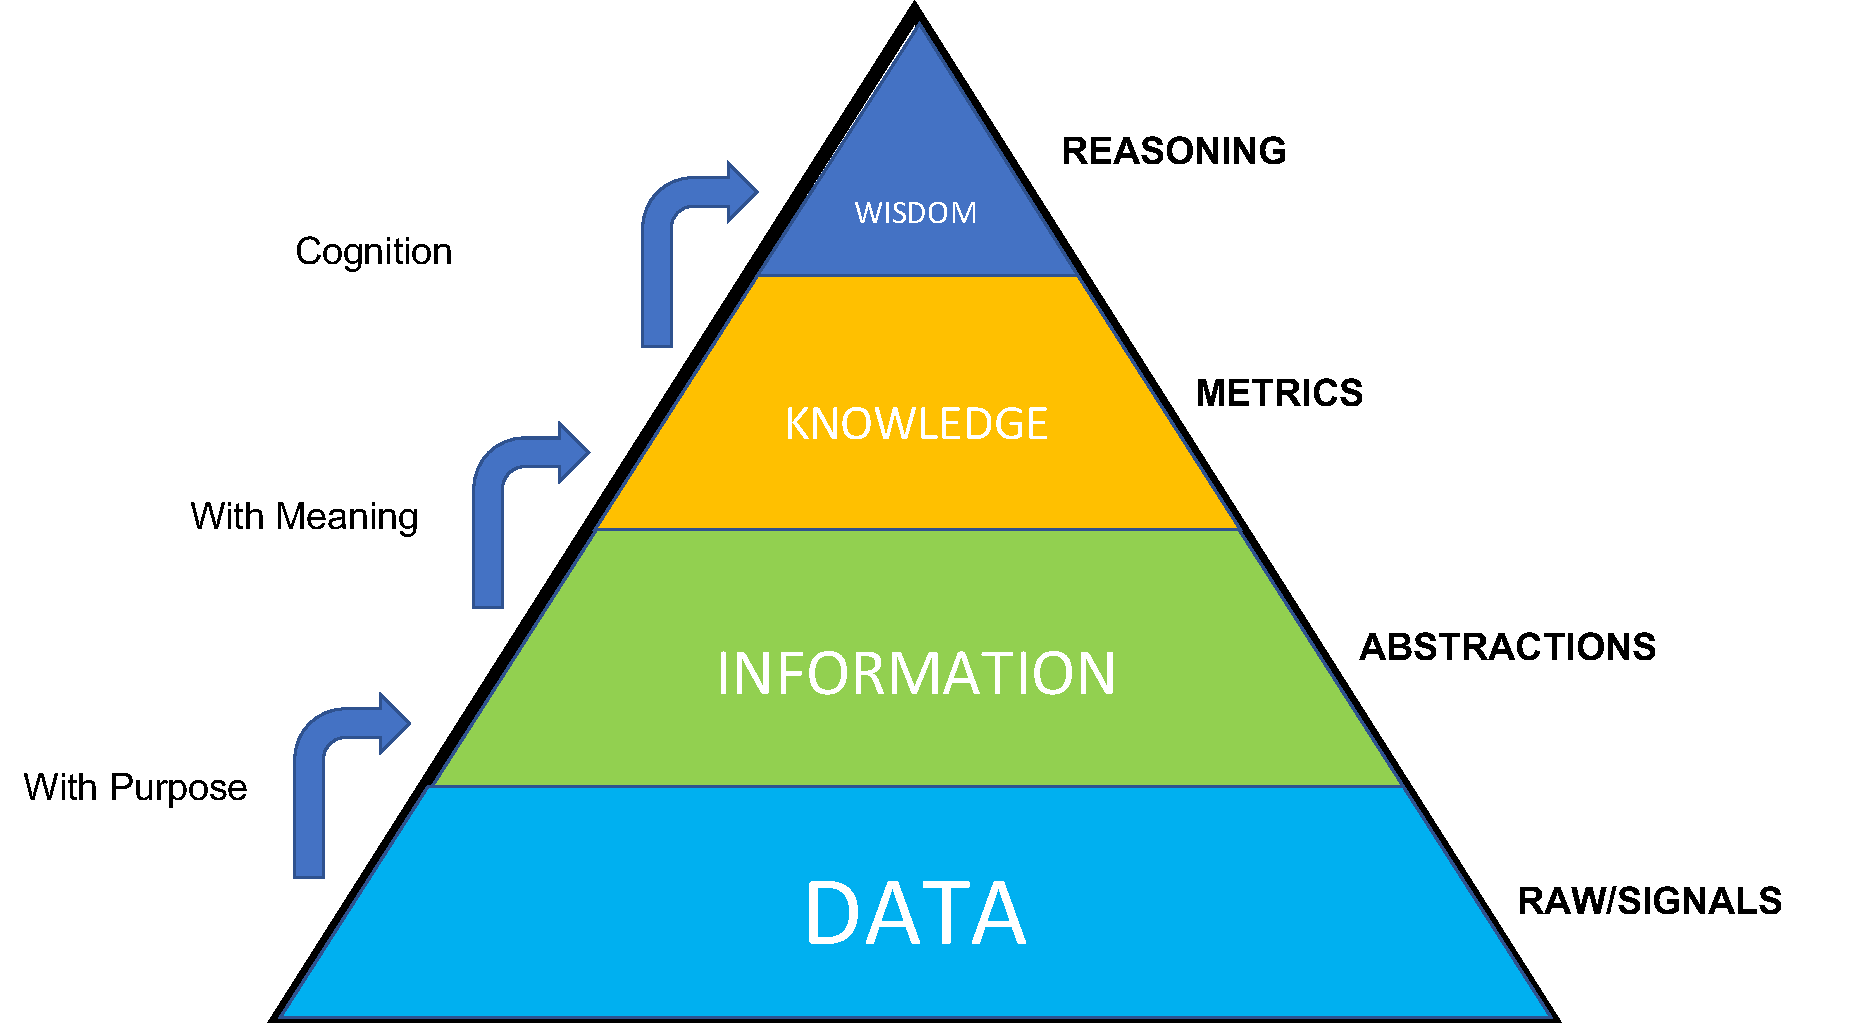
\includegraphics[width=\columnwidth]{DIKW.pdf}
    \caption{The DIKW pyramid}
    \label{fig:dikw}
\end{figure*}

In attempt to develop metrics and pipelines, one has to reflect on one of the fundamental frameworks about operations on data, that is the \textbf{Data , Information, Knowledge and Wisdom} model\cite{rowley2007wisdom}.In this dissertation I posit and demonstrate through case studies, that for any reasoning about subjective perceptions , you need to develop frameworks that extract knowledge from data in a format that is aligned with the ontological framework of the application. In the context of this dissertation, ontology implies a set of concepts, definitions and relations between entities defined around a common set of axioms. I show that if a set of relations and definitions of concepts in the area of intervention are present, `a' solution can be reached provided that systems are designed to interpret metrics extracted from the data in relation to the ontology of the area of application. But to reach this step, the data needs to pass through the 4 layers of the DIKW pyramid model.

In this model, the most foundational layer consists of the pure form raw \textbf{data or signals} that come from a source. If we are measuring subjective perceptions of humans, this source needs to be tied back to humans in some way. \red{Change this sentence} The data needs to be generated as a result of some human-human interaction or as a result of deliberate human input as response to their perception of some event. In this dissertation, I present various data sources and methods of collecting and curating data, which pertain to human-human interactions or human responses. 

The \textbf{information} layer is the result of the fact that any process done on the data is with a sense of purpose or an end goal. For example, if the goal is to understand how humans exchange messages at times of distress, you would most certainly need to express the raw information about sender and recipient of messages into some form of a networked abstraction. The abstraction preserves the organization of data, but at the same time allows information to be operated on. As a result, almost always the output of this process is some form of a data abstraction. You need to attach some meaning to the patterns in the information to extract knowledge about the fundamental processes that you want to measure.

\textbf{Knowledge}. Defining knowledge has been an ongoing effort in the field of philosophy. But in the context of information science, knowledge involves collation of diverse sources of information and  mix of contextual information, values and metrics to deliver a coherent understanding of the real world. For example, if you need to know the most popular user among a social network of users exchanging messages; you would look for the most central user in the network(abstraction) along with several other temporal and structural metrics to arrive at a few candidates. In this particular case, these metrics, along with the context of the social network's design, dawns the meaning of popularity. 

The final layer needs a cognitive process and an ontological framework, to extract actionable insights, which we can call \textbf{wisdom}. By classical definition of ontology, it defines properties of and relations between objects or concepts. For this very reason, these ontological frameworks need to be originating from the fields of intervention.  In our example, lets assume we need to get some insights about the dynamics of popular users. Particularly in the context of optimizing advertising delivery. For example we need to understand how a particular piece of advertising, might percolate through the network if certain popular users advertise it~\cite{li2012diffusion}. However , to arrive at these insights we need to be grounded in the ontological frameworks of epidemiology, network physics and depending on the application, advertising or meme theory. Then using the abstractions of social networks, the metrics derived from them, and the ontological basis of all the aforementioned fields, one can design a pipeline that could deliver us these insights with reasonable accuracy. 

Figure \ref{fig:dikw} shows an illustration of the adopted version of Rowley's DIKW model, which I would refer back as a repeating motif for my dissertation.

\subsection{Data}
Data is one of the most fundamental contribution of this work. To develop frameworks around quantification of human perceptions, such that we can do impactful interventions from this approach, we first need to make sure we formalize how we acquire, clean and condition our data. The most base level of this pyramid is the data that the frameworks would work with in order to progress on these lines. I work with diverse forms of data such as textual data , video data and image data to understand how these might exhibit signatures of human perceptive processes. The relation between data and subjective attributes needs to be examined using some proxy. For this reason, my research involved collecting data from sources where either human to human interactions happen or the data is generated on account of a human expressing their opinion about a subjective quality like beauty of a place, or how much someone ``likes'' an image or a video.

\subsubsection{Interaction Data}
In the first case study of this dissertation focusses on is online support communities, where human to human interaction is at the centre of the utility of these communities. It has been shown through several studies in medical informatics, that these communities play a very important role in providing support and respite in times of distress~\cite{allen2016long}~\cite{mo2012developing,pendry2015individual} ~\cite{bartlett2011investigation,izuka2017stroke}~\cite{hobbs2016online}. The communities are especially helpful when it comes to people suffering from long term illnesses or mental health issues.
The key element that impacts the users is the perceived social support~\cite{nambisan2011information}, which delivers people in distress a sense of belonging to a group and empathy from the fellow supporters. 
To understand how users on these communities perceive social support, I work with data acquired from online health forums, where users share, give support and ask for support. I look at communities that deal with long term conditions like Lung illnesses, and communities where mental health patients seek support~\cite{joglekar2018online}. The data spans across a duration of 10 years, containing peer to peer support interactions of more than 30,000 users. I also crawled a popular forum based social network called reddit \footnote{\url{www.reddit.com}} to acquire a peer to peer support forum data regarding mental illness and suicidal thoughts. The data covers discussions about more than 30,000 calls to support, and incorporates the complete structure of the way people respond to these calls. 

\subsubsection{Media data}
The other facet of my work looks for quantification of how we perceive physical spaces. Whether a street is considered beautiful is a matter of subjective opinion, yet research has shown that there are specific urban elements that are universally considered beautiful: from greenery, to small streets, to memorable spaces~\cite{alexander1977pattern, quercia2014aesthetic,salesses2013collaborative}. These elements are those that contribute to the creation of what the urban sociologist Jane Jacobs called `urban vitality'~\cite{jacobs1961death}. Apart from vitality, these motifs in urban environments are also highly correlated with feeling of well-being, health and safety~\cite{kaplan1989experience}. There have been studies where people have tried to use crowd sourcing to acquire subjective ratings of images~\cite{seresinhe2015quantifying} which have shown some reasonable progress on this front. But the real gap in these studies is understanding the impact of urban elements on the perception of these subjective qualities. E.g. How much does presence of a green garden affect the subjective rating of beauty of that particular area. For this reason, I work with google street view data and subjective ratings of various places around the world~\cite{naik2014streetscore}, with the aim to understand,  how people perceive the sense of beauty in urban areas. Then using the ontological basis of urban design and architecture, developed by a detailed literature review, I aim to develop machine learning pipelines that can suggest interventions to change perceptions of physical spaces.

\subsection{Abstractions}
The act of aggregating information from data, almost always involves building organized abstractions. Throughout my dissertation, I either repurpose well known abstractions in computer science or develop my own using tools from fields like computer vision and Information theory. For the first study, I incorporate user meta data and the textual data of their activity, to build organized networked abstractions representing the conversation structures on the support forums. I use these abstractions to evaluate global and local structures in support communities, which would be discussed in detail in Chapter \ref{chap:Utility_support} and \ref{chap:structure_support}. 
  
While working with media data, I use several pixel level abstractions to segment and group semantically similar pixels. I also use several state of the art object and scene detection to extract semantic information from an image, with the aim at analysing correlations with the perception of subjective attributes of images with these metrics. I also use deep convolutional networks and generative models, to abstract out a representation of beauty. A more detailed discussion of these abstractions would be done in the later chapters (Chapter \ref{chap:quant_perception}).  

\subsection{Knowledge}
For extracting knowledge, we need to first associate meanings to certain computable metrics that we obtain from the abstractions. As discussed in the previous example, it could be as simple as associating the property of ``popularity'' to the metric of centrality. In my case, I develop several of these metrics to related subjective properties with measurable structures in data. Some of these metrics are based on intuitions which I validate, and some based on extensive literature survey. To give an example, I develop the concept of anchored triads, which combines local structures in interaction graphs of users, with the role of a user in a supportive conversation, to understand how these conversations evolve.

\subsection{Wisdom}
Finally the wisdom , in definition underlies insights that come for experience. The experience could come simply from the scale of data or from cross disciplinary literature that puts forth theories of subjective experience. E.g. The theory of social support puts forth four categories of social support 1)Affective/Perceived 2)Instrumental 3)Informational 4)Appraisal. Each type has its own specific traits. My dissertation looks at these theories from the lense of computational social science, and develops processes to quantify signatures of affective support.

\section{Research Thesis and Questions}
I would like to put forth the thesis that I would like to examine through this dissertation. The overarching thesis question of interest is: 

\vspace{1cm}
\noindent\fbox{\begin{minipage}[t][2\height][c]{\dimexpr\textwidth-2\fboxsep-2\fboxrule\relax}
        How do we quantify perceived quantities from data, if the data source is human and the scale is large?    
\end{minipage}}
\vspace{1cm} 

But this thesis question is quite open ended, and answering it in a generalized manner seems impractical in the scope of one Ph.D. For this reason, I need to first contextualize my work in the realm  of practical applications, by deriving more focussed research questions, such that I can acquire data and test my hypothesis in an effective time bound manner. More so, being an impact driven person, I would like to focus on applications which have the potential to have real world impact, either through interventions or through inspired interest in the field.

\subsection{Supportive Interactions on the web}
Humans are social animals in every aspect. The presence of social support systems in ones lives have shown to have huge quantifiable benefits. From speeding up recovery in cases of post-partum depression or in the cases of cancer survivors~\cite{collins1993social,dunkel1984social,baron1990social} , to signs of positive turn around among patients suffering from alcoholism and depression~\cite{peirce2000longitudinal,brown1986social}, social support is a key predictor of positive prognosis for patients under distress. With the advent of internet, a lot of communities have sprung up, which provide a rich platform for patients to interact, exchange support as well as provide a perceived sense of community. These communities are moderated, only to an extent to curb toxic behaviour, but other than that are largely free form. Due to a very homogenous membership, where most members have either gone through or are going though similar distress, there is an emergent sense of support and affective empathy~\cite{de2016stroke}. The idea of this case study was to quantify how supportive processes evolve over these communities, using abstraction methods from the fields of network science. The hope in doing so, is that the communities would be better poised to tackle any disturbances in the dynamics of these supportive communities as well as quantify the net utility these communities offer to the users. 

The investigation of these would lead me to form the following research questions 

\noindent\fbox{\begin{minipage}[t][2\height][c]{\dimexpr\textwidth-2\fboxsep-2\fboxrule\relax}
        \textbf{RQ1} \textsl{What are the characteristics of conversations on health support communities?}   
\end{minipage}}

\noindent\fbox{\begin{minipage}[t][2\height][c]{\dimexpr\textwidth-2\fboxsep-2\fboxrule\relax}
        \textbf{RQ2} \textsl{What is the nature of dialogue in supportive communities?}   
\end{minipage}}
\noindent\fbox{\begin{minipage}[t][2\height][c]{\dimexpr\textwidth-2\fboxsep-2\fboxrule\relax}
        \textbf{RQ3} \textsl{Are there any discriminative macroscopic signatures in supportive conversations?}   
\end{minipage}}
\noindent\fbox{\begin{minipage}[t][2\height][c]{\dimexpr\textwidth-2\fboxsep-2\fboxrule\relax}
        \textbf{RQ4} \textsl{Are there any discriminative local signatures in supportive conversations?}   
\end{minipage}}
\vspace{1cm}

To achieve this I first had to collect data from two different communities designed for online social support. The first community is dedicated for patients suffering from chronic lung diseases, such as Asthma or Chronic Obstructive Pulmonary Disorder (COPD). This community was moderated by self appointed moderators, and everyone on this community was either a survivor or a patient of these diseases. This community allowed patients to ask questions about symptoms and home remedies and sometimes just bond over social interactions. The second community I worked with dealt with people suffering from chronic depression and suicidal thoughts. This community was a safe haven for such people to vent out suicidal thoughts and get support from peers to manage these sudden flares of thoughts of self harm. 

Through these two communities, I develop a pipeline to analyse the peer to peer interactions using abstractions derived from network science. The abstractions try to mimic the conversation structure which allows me to probe the evolution of such conversations both in terms of macroscopic properties as well as local interactions between users. I also develop metrics inspired from psychology and sociology literature to quantify how these interactions can be qualified as supportive or non supportive. Through a data driven analysis, I establish confidence on these metrics. Through this process, I also report my findings about the dynamics of users on these communities and key properties of user roles. I find that these conversations have a distinct nature when compared against regular baseline conversations over the web, and these distinct signatures could one day be used to curb toxicity as well as improve the support community interface.

\subsection{Leveraging aesthetic perceptions of real spaces}
Urban aesthetics and presence of certain elements in the physical spaces that we use, have shown to have lasting effects on our mental health\cite{seresinhe2017using} and physical well being\cite{ball2001perceived,giles2005increasing}. However, with the advent of large scale data access, and machine learning techniques, we have a unique opportunity to quantify what exactly comprises of urban aesthetics.
In the next part of my dissertation, I aim at using the scale of the internet to try and improve how our cities are perceived. In this study, I investigate the following research question: 
\noindent\fbox{\begin{minipage}[t][2\height][c]{\dimexpr\textwidth-2\fboxsep-2\fboxrule\relax}
        \textbf{RQ5} \textsl{Can crowdsourcing and machine learning help us quantify how humans perceive aesthetics in urban settings?}   
\end{minipage}}

\noindent\fbox{\begin{minipage}[t][2\height][c]{\dimexpr\textwidth-2\fboxsep-2\fboxrule\relax}
        \textbf{RQ6} \textsl{Can machine learning leverage this quantification to improve aesthetics of urban spaces?}   
\end{minipage}}

\noindent\fbox{\begin{minipage}[t][2\height][c]{\dimexpr\textwidth-2\fboxsep-2\fboxrule\relax}
        \textbf{RQ7} \textsl{Do humans and practitioners find these interventions worth the effort?}   
\end{minipage}}
\vspace{1cm}

Crowdsourcing is a method through which one could get inputs, subjective or otherwise, about a particular set of questions from a large number of real humans using the internet. In return the participants could be offered a tangible compensation, or in some cases, a gamified incentive. 
The \textbf{RQ5} motivates me to investigate if we can use crowdsourcing to quantify how people perceive urban spaces. Research has shown that if a large number of people could vote on a set of images, regarding their aesthetic quality, a trend emerges that favours some objective metrics of beauty\cite{datta2008algorithmic,612644,quercia2014aesthetic}. Can we link these metrics to urban elements? For this reason we work with google streetview images, where real people vote on aesthetic value of images through a large scale crowdsourced study. After evaluating for statistical trends in preference of aesthetic urban images amongst the voters, we answer \textbf{RQ5} by training a deep convolutional neural network model, which can discern between an aesthetically pleasing and unpleasant urban scene with a high degree of accuracy. Once we have a model that could ``detect'' beauty in urban scences, we could then use machine learning and deep learning techniques to understand how different urban elements relate to the notion of beauty (\textbf{RQ6}). I further try to build a tool, which could use the quantified notion of beauty in urban spaces, to hint practitioners about possible actions to beautify any given urban space. These hints are given in the form of suggested changes in different popular urban design metrics, which makes the whole process legible to practitioners in the field. In the pursuit of answering the \textbf{RQ6} and  \textbf{RQ7}, I propose deep neural network and generative adversarial network models to make an end-to-end pipeline which can be then used to visualize how different urban elements affect the perception of beauty in the real world.


\section{Thesis overview and original contributions}
In Chapter 2, I examine how supportive communities evolve and sustain over a long period of time. I show presence of an anti-rich club effect on these support groups, which implies that experienced users are more interested in helping new comers rather than forming a clique of their own. I define a quantitative metric for ``expertise'' and show that as one becomes adept, one becomes more willing to help. All these original insights point towards answers for \textbf{RQ1} and \textbf{RQ2}. In Chapter 3, I look at global and local structures of supportive conversations. I show that mapping the conversation exchanges onto a topological structure exhibits keen preference for local supportive structures, which I call ``anchored motifs''. I discuss the utility of such a model of support conversation and draw parallels with the offline model of community support(Chapter 4) as per the mandate of \textbf{RQ3} and \textbf{RQ4}. 

In the second study, I investigate utility of perceptions of real world places through a crowd sourced rating of google street view images. As per \textbf{RQ5}, I develop models to extract the perception of the crowds using data driven inference methods(Chapter 4). 
I then show that a general pattern of beauty in urban spaces can be learnt through a crowd sourced opinion and based on this finding, I develop a generative model to simulate beautification of urban spaces by using deep learning(Chapter 5). I validate the quantification of perception of real-world beauty using crowd validation. I contribute a way to use computer vision techniques to abstract out beautification process into explainable metrics used by architects and urban planners. The final contribution is a demo web application, that allows practitioners to examine and validate the utility of such a end to end system that captures citizen perceptions for urban design. These contributions are motivated by \textbf{RQ5} and \textbf{RQ7}. 
I close by enumerating the different research problems and future directions that my work would pursue as a early career scientist(Chapter 6)



\section{List of peer reviewed publications}

I would like to list all the publications which resulted from the past 4 years of work, as well as collaborations I was able to strike with a diverse group of researchers. The author lead publications have influenced different chapters of this dissertation.

\subsection{Original author contributions}
List of papers, published and in review, which were led by the author or where the author had fundamental contribution

\begin{enumerate}
    \item \textbf{Joglekar, Sagar}, Nishanth Sastry, and Miriam Redi. "Like at First Sight: Understanding User Engagement with the World of Microvideos." International Conference on Social Informatics. Springer, Cham, 2017.
    
    \item \textbf{Joglekar, Sagar}, et al. "How online communities of people with long-term conditions function and evolve: Network analysis of the structure and dynamics of the asthma UK and British lung foundation online communities." Journal of medical Internet research 20.7 (2018).
    
    \item \textbf{Joglekar, Sagar}, et al. "Online discussions about mental health in Reddit exhibit signatures of supportive conversations" Under Review
    
    \item \textbf{Joglekar, Sagar}, et al. "FaceLift: A transparent deep learning framework beautifying urban scenes" Under Review
    
    \item Kauer, T., \textbf{Joglekar, S.}, Redi, M., Aiello, L. M., \& Quercia, D. (2018). Mapping and Visualizing Deep-Learning Urban Beautification. IEEE computer graphics and applications, 38(5), 70-83.
    
\end{enumerate}

\subsection{Collaborative author contributions}
List of papers, published and in review, where the contribution was significant, but were not led by the author

\begin{enumerate}
    \item Bhatt, S., \textbf{Joglekar, S.}, Bano, S., \& Sastry, N. (2018, April). Illuminating an ecosystem of partisan websites. In Companion of the The Web Conference 2018 on The Web Conference 2018 (pp. 545-554). International World Wide Web Conferences Steering Committee.
    
    \item De Simoni, A., \textbf{Joglekar, S.}, Taylor, S. J., Patel, A., Duschinsky, R., Coulson, N., ... \& Evans, M. J. (2017). Structure and dynamics of online patients’ communities: the case of Asthma UK and BLF online fora.
    
    \item YOUNG, A. P., \textbf{Joglekar, S.}, GARIMELLA, K., \& SASTRY, N. (2018). Approximations to Truth in Online Comment Networks.
    
    \item Agarwal, P , \textbf{Joglekar, S.}, Papadopoulos, P., , SASTRY, N. \& Kourtellis, N. (2018) Hyper-partisan websites: Personalization of user experience on
    polarized websites.
    
    
    \item Raman, A , \textbf{Joglekar, S.}, De Christofaro,E., SASTRY, N. \& Tyson, G. (2018) Tooting Your Own Horn: Exploring the Impact of
    Decentralisation on the Mastodon Social Network.
    


\end{enumerate}









%_____________________________________________
% Vine paper based chapter 2
%
\chapter{Engagement and Attention Budgets}

\graphicspath{{Chapter2/plots/}}
\begin{quote}
    
    \textsl{In an information-rich world, the wealth of information means a  dearth of something else: a  scarcity of whatever it  is that information consumes. What information consumes is  rather obvious: it consumes the attention of its recipients. Hence a wealth of information creates a poverty of attention - Herbert Simon}\cite{simon1971designing}
    
\end{quote}
We live in an information rich world, where the notions of engagement, entertainment and social connection have all been migrated as close to the user as possible. Along with the portability of content consumption, content creation has also become a lot more portable and accessible because of the ever improving quality of handheld devices and their native cameras. In such an environment the headlining quote of Simon Herbert is ever so relevant. This wealth of information has created a poverty of attention. As a side effect, the poverty of attention has driven development of content formats that by design require low attention budgets. Examples of these could be Vine, Instagram stories, Whatsapp Stories, Facebook stories,  which allow users to create short ephemeral videos, which get deleted automatically after 24 hours. The user experiences are also designed around user experience of rapid scrolling, only to stop for a quick peek. 

In the context of this dissertation, it is interesting for me to investigate how users on social media platforms make decisions about whether to engage with a particular piece of content or not. More specifically, do specific user perceptions play a role in how they interact with content on these platforms. To that extent, I hypothesize that this decision is governed by two factors. The first is the state of \textbf{social embeddedness} of the consumer, such that being a particularly popular person increases one's chances of getting engagement on the content. The other factor is the \textbf{aesthetic and perceptive attributes} that make a content `catchy', such as an upbeat background music, presence of attractive faces, aesthetic framing of content, photographic structure and other attributes. Intuitively it seems plausible to track down the contributions of each of these factors if we can acquire a large enough data of social media content and their engagement metrics. There are several of such user generated content creation platforms that could be focused upon for this study, such as Instagram (1 billion users worldwide), Facebook (1.74 billion users) , Vine (200 Million active users as of 2016) or Snapchat (400 million  users). The scale at which these platforms function, makes modelling of how users spend their attention budgets, an interesting problem. This motivations is ever more crucial when recent studies have shown a high correlation between usage of these medias and mental health\footnote{https://www.bbc.co.uk/news/health-39955295} issue in young adults\cite{lup2015instagram,holland2017strong}

Although most user-generated video platforms have placed some form of limit on the duration or size of videos (e.g., YouTube had a 10 minute limit, which has since been softened to a `default' limit of 15 mins\footnote{\scriptsize https://techcrunch.com/2010/12/09/youtube-time-limit-2/}), the extremely short duration time limits of Vine, Shapchat, Instagram stories etc has led to the coining of a new term: \emph{micro videos}. Some media commentators have argued that the restrictions imposed by the micro video format could fundamentally change the way we communicate~\cite{bbc}. Indeed, it has been argued that Vine has had a significant cultural and technological impact far beyond its user base, generating several widely shared memes in its short lifetime\footnote{\scriptsize http://www.theverge.com/2016/10/28/13456208/why-vine-died-twitter-shutdown}, and inspiring other social media platforms to adopt this format\footnote{https://www.pewresearch.org/fact-tank/2013/06/20/instagram-vine-and-the-evolution-of-social-media/}. The makes Vine, a natural and crucial choice to study these processes on.


At the same time, as the format is still very new, virtually all major micro video platforms are experimenting with the format, making significant changes in the last year. For instance, Instagram extended the limit from 15 seconds to 1 minute\footnote{\scriptsize http://www.theverge.com/tech/2016/3/29/11325294/instagram-video-60-seconds}. Vine is undergoing a major overhaul -- Twitter recently said it would close down the Vine website and community. The new version of the Vine app retains the 6.5 second video format, but the videos will be published directly on Twitter's feed and thus more closely integrated with its social network\footnote{\scriptsize http://www.theverge.com/2017/1/5/14175670/vine-shutting-down-rebrand-download-archive}. 

In the context of these developments, it was crucial to understand how these media formats might change the landscape of user generated content. Understanding the dynamics of interactions of users with this format might have large impact when it comes to social media messaging and marketing strategies. Hence I examine this dimension of user perception of this media, along two dimensions: 
\begin{itemize}
    %\item[\textbf{RQ1}] How do micro videos differ from other user generated content (e.g., Videos on YouTube, Images on Flickr?)? 
    \item[\textbf{RQ1}] What are the relative roles of  social and content quality factors in driving engagement and popularity in micro-videos?
    \item[\textbf{RQ2}] How does the strict time limit impact video quality, and user engagement (both as creators and consumers) with such videos? %And as a corollary, do longer time limits change quality or user engagement?
\end{itemize}

I answer these questions from an empirical perspective, using a dataset of nearly all ($\approx 120,000$) Vine videos that were uploaded to one of the 18 globally available channels on Vine during an 8 week period. We complement these with other datasets including a curated dataset (\emph{POP12K}) of 12,000 popular Vine videos, as well as samples from other micro-video platforms such as Instagram.

To address \textbf{RQ1}, we take the three metrics of popularity which are collected -- counts of loops, reposts and likes -- as quantification of the \emph{collective} user engagement of the consumers of a video, and ask to what extent the content- and social network-related features affect these metrics. To answer this question, we develop a novel pipeline, that helps us understand individual influences of different features selected, on the popularity of a content item.
We train a random forest classifier that, given a threshold for a metric of popularity, is able to able to distinguish items on either side of the threshold into popular and unpopular classes  with high accuracy, precision and recall, using the features we have identified. The relative importance of different features then gives an indication of the extent to which those features affect the metric under consideration. We progressively consider higher and higher threshold values for videos to qualify as popular or engaging, and thereby identify trends and changes of relative importance of different features. Interestingly, we find that as the threshold for popularity becomes more and more stringent, features that represent quality of the content become collectively as important as social features such as the number of followers. Echoing an effect also observed in Instagram photos~\cite{bakhshi2014faces}, we find that presence of faces in vine videos significantly increases engagement, and is the most important content-related factor.

Next, to explore \textbf{RQ2} we look at how the quality of the video varies over time in micro-videos, and discover a \emph{primacy of the first second} phenomenon: the best or most salient parts of the video, whether in the aesthetic space or affect (sentiment) space, are more prevalent in the initial seconds of the micro video, suggesting that the authors are consciously or subconsciously treating micro-videos similar to images -- in the initial part, the video is composed with aesthetics and affective quality in mind, resulting in a higher quality level; but quality declines as the video plays over time. Furthermore, echoing the primacy of the first second phenomenon, we find that the quality of the first seconds of the video are as effective as the quality of the whole video in predicting popularity/engagement. Fig.~\ref{fig:Vine_samples} shows examples of these effects through two videos in our dataset of popular videos. In both videos, we observe content quality deteriorate over time, illustrating the primacy of the first seconds. 

\begin{figure}[!tbh]
    \centering
    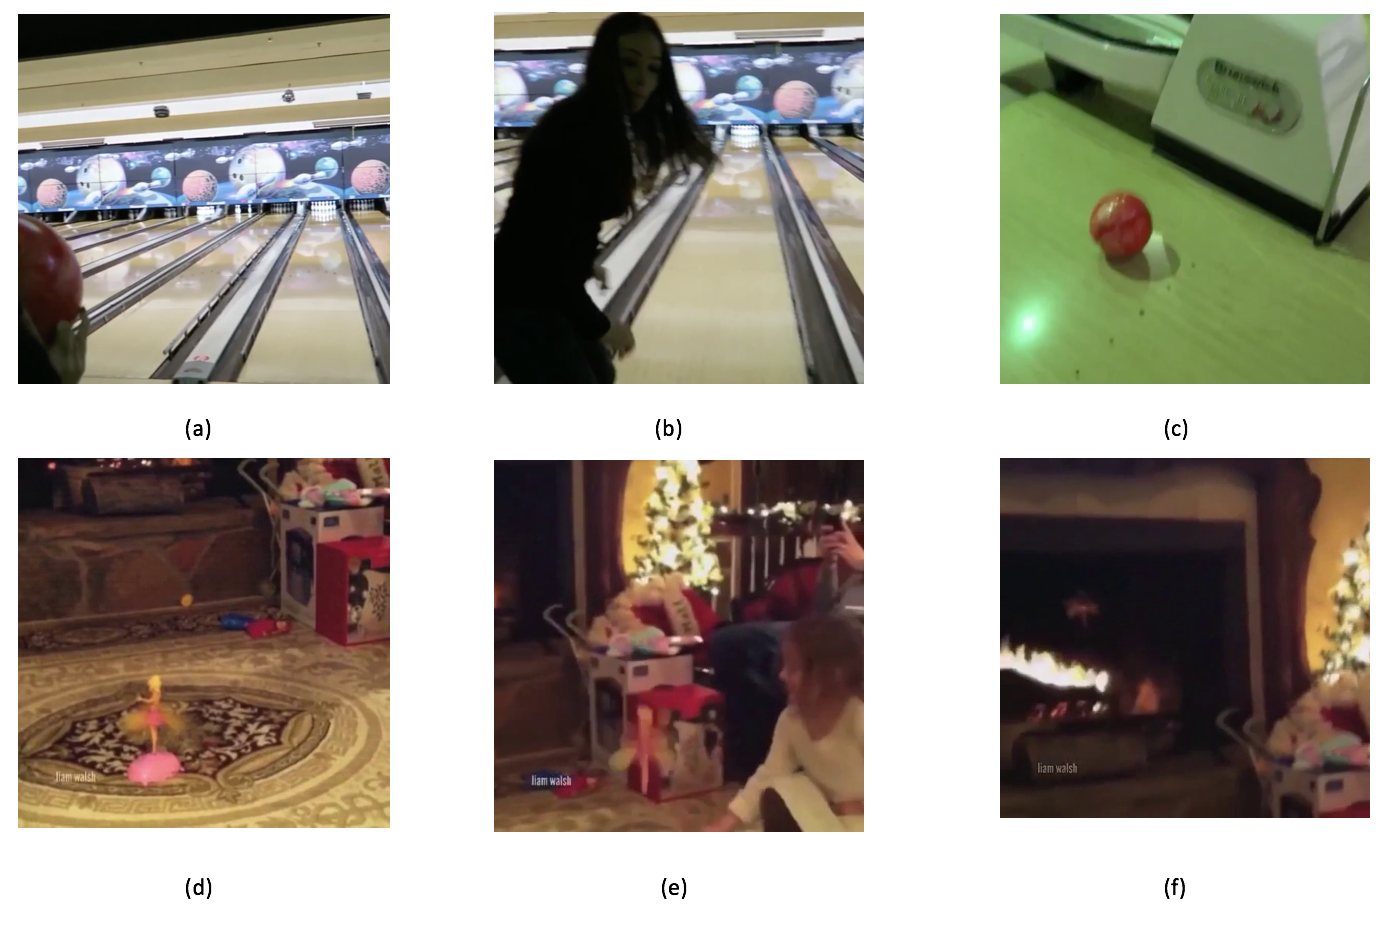
\includegraphics[width=0.7\columnwidth]{Vine_samples2.png}
    \caption{\textsl{ Vine Samples from first, second and thirds one thirds of the video. Images (a) , (b) and (c) show a progressive drop in brightness and sharpness due to shaky camera. Images (d) (e) and (f) shows a progressive drop in contrast.}}
    \label{fig:Vine_samples}
\end{figure}

We confirm these computationally acquired findings with real user impressions by designing a survey which was answered by 115 respondents: Over 66\% of users react to (like/comment on) content from their friends, making social interaction a significant part of content consumption; and 44\% of users form opinions about videos in the first few seconds, validating the observed primacy of first seconds effect. Our survey also suggests that platforms such as Vine are seen as less professional and more immediate formats than, say Flickr images or YouTube videos, providing support to David Pogue's  position that micro videos are a new kind of user-generated content~\cite{pogue13}, and therefore should be treated differently when it comes to user engagement.



\section{ Related Work}
this work closely relates to those works  in machine vision that infer intangible properties of images and videos. While  computer vision frameworks typically focus on analysing image semantics using deep neural networks \cite{krizhevsky2012imagenet}, researchers have started exploring concepts beyond semantics, such as image memorability \cite{isola2011makes}, emotions \cite{Machajdik}, and, more broadly, pictorial aesthetics \cite{datta2008algorithmic,luo2008photo,goodSelfie}. 
This work specifically focuses on on-line visual content collected from social media. Researchers have shown that, by leveraging social media data in combination with vision techniques, systems can estimate visual creativity \cite{redi20146},  sentiment \cite{wang2015inferring,jou2015visual} and sarcasm \cite{schifanella2016detecting}. %Recent studies have also shown that vision techniques can be employed to detect the ambience of the places visited by the subject of a profile picture  \cite{redi2015like}, the home and vacation location of the owner of a photo album \cite{zheng2015towards}. 

More specifically, our work closely relates to research that combines social media studies and computer vision to analyse popularity and diffusion for social media posts: for example, Zhong \textsl{et al.} were able to predict the number of post ``re-pins''  given the visual preferences of a Pinterest user \cite{predictingPintrest}; recent work \cite{Mazloom:2016:MPP:2964284.2967210} has also used multimodal features to predict the popularity of brand-related social media posts. Different from these works which focus on prediction,  this work looks at understanding user engagement. 

Media popularity prediction studies generally focus on non-visual features.  For example, \cite{Yamasaki:2014} used textual annotations to predict various popularity metrics of social photos. Social metrics such as early views \cite{pinto2013using} or latent social factors \cite{nwana2013latent} have also been used to effectively estimate video popularity. However, the fact that many popular media items may not depend on the social  network~\cite{Cha2009Flickr} suggests that intrinsic media quality is an important factor for diffusion, engagement and popularity, which we explore in this work.

Recent work in the field has explored the importance of visual content in analysing popularity: \cite{totti14impact} analysed the visual attributes impacting image diffusion,  and \cite{schifanella2015image} studied relations between image quality and popularity in on-line photo sharing platforms.  Bakhshi et al  \cite{bakhshi2014faces} showed that pictures with faces tend to be more popular than others. Similar to our work, researchers have used computer vision techniques to estimate image popularity in Flickr \cite{Khosla:2014}. Moreover, a work done by Fontanini et.al \cite{fontanini2016web} explores the relevance of perceptual sentiments to popularity of a video. 
Unlike these works, we  explore content features to fully understand user engagement and popularity in micro videos, a new form of expression radically different from both the photo medium and the video medium.% We motivate our study by providing quantitative evidence for such radical novelty introduced by Vine videos, running a cross-platform comparison study based on audiovisual features.  

Micro videos are relatively new, so work specifically on micro video analysis has been limited. Redi \textsl{et al.}~\cite{redi20146} quantify and build on the notion of creativity in micro-videos. A large dataset of 200K Vine videos was collected by Nguyen et.al \cite{nguyen2016open}, focusing on analysis of tags. Closest to our work is Chen \textsl{et al.}~\cite{Chen:2016:MTM:2964284.2964314} who use multimodal features to predict popularity in micro videos. However, although we use popularity prediction as an intermediate tool, our focus is on understanding impact and importance of different features in determining popularity or engagement. To this end, we introduce a novel methodology 
%(\S\ref{sec:methodology}) 
that allows understanding up to which point social features are prominent over content features. Additionally, we demonstrate the ``immediacy" of engagement with micro videos by showing that the content from the first two seconds of the video is just as good at predicting  popularity as the entire content 
%(\S\ref{sec:first-seconds})
. Collectively, these results allow us to characterise Vine as a new medium of expression, different from previous work.




\section{Introduction to Datasets}

Micro videos were pioneered and popularised by Vine\footnote{\scriptsize http://vine.co}, which was launched in 2012. Vine videos are constrained to a maximum length of 6.5 seconds. Videos are typically created using the mobile app and posted on user's profile which can be followed and shared by other users within the app or the website. %Instagram on the other hand, in early 2016,  introduced videos with a relaxed time duration constraint of up to 1 minute, which has seen a sudden surge in usage. 
We stress most of our work on videos sampled from Vine, complemented by %YouTube, Flickr and 
Instagram data, which will be introduced as appropriate. The rest of this section gives details about the Vine datasets.




\subsection{Dataset description}\label{sec:dataset}
\begin{table}[hbt]
    \centering
    \begin{tabular}{l|cccc}
        \thead{Dataset} & \thead{\shortstack{Posts\\ (total)}} & \thead{\shortstack{Loops/Views\\ (median)}} & \thead{\shortstack{Reposts\\ (median)}} & \thead{\shortstack{Likes\\ (median)}} \\
        \hline
        POP12K & 11448 & 318566  & 2173 & 7544  \\
        ALL120K & 122327 & 80 & 0 & 2 \\
        %INSTA15k & 14568 &  93  & N/A  &  40\\
    \end{tabular}
    \caption{Summary characteristics of datasets used}
    \label{tbl:dataset}
\end{table}


The data used in this work is summarised in Table~\ref{tbl:dataset}, and was collected in two phases as described below: 

\paragraph{Popular videos dataset} First, we collected $\approx$ 12,000  videos which have been marked by Vine as `popular', by tracking the `popular-now' channel\footnote{\scriptsize https://vine.co/popular-now} over a three week period in Dec 2015, and downloading all videos and associated metadata once every six hours, and removing any overlapping videos from the previous visit. The crawling period was chosen to ensure that consecutive crawls have an overlap of several videos, and this sufficed for all visits made to the website during the data collection period; thus the dataset we collected is a complete collection of all `popular-now' vines during the 21 days under consideration. %After removing all duplicates, a total of \textbf{XXX} popular videos were collected. 

Vine does not disclose the algorithm used to mark a Vine as popular; yet we observe (see Table~\ref{tbl:dataset}) orders of magnitude more loops, reposts and likes in the popular-now dataset than in the non-popular dataset. Thus we believe that the algorithm used by Vine to select vines for the 'popular-now' channel is strongly affected by the numbers of loops/revines/likes. Note that the numbers of loops etc. were collected at the time of crawl, within a maximum of six hours of being posted on the 'popular-now' channel, which limits the possibility that the counts increased \emph{as a result} of being featured on the popular-now channel. In the rest of the chapter, we use the counts in the popular-now dataset to calibrate the definition of `high engagement'. While there is a possibility that this is a biased proxy for global engagement, it nevertheless provides a baseline against which to compare all videos.

\paragraph{All channel videos dataset} In the second phase, we collected 
videos accessible from each of the 18 global Vine channels or categories%\footnote{https://vine.co/api/timelines/channels/<channelNumber>/recent?size=100} 
over a period of {8 weeks} from {Aug 16 to Oct 12  2016}. Again, a crawling period of six hours was chosen for consecutive visits to the same channel, and the 100 most recent vines were fetched with each visit. The number 100 was a result of an API limit from Vine. 
%As shown in Fig.~\ref{fig:download-fraction}, the  vines returned has a significant overlap with vines fetched from the previous visit. 
Our dataset captures nearly all videos uploaded to Vine and assigned to a channel. The only exception is the extremely popular comedy channel, for which we nearly always find more than 100 new videos (we only download the 100 most recent videos for the comedy channel). In total, this results in a dataset of $\approx$120,000 videos. We track  loop, revine and like counts  over time, periodically updating each video's counts every three days until the end of  data collection. At the last tracking cycle, we have metadata for each post for  3 weeks after initial  upload.

Note that while we obtain nearly all videos across the channels, our dataset does \emph{not} capture  \emph{all} videos uploaded to Vine -- Vine creators do not need to assign a video to a channel. However, due to the Vine platform structure,  vines that are not in channels have near-zero probability to get seen by other users apart from the followers. % and we do not discover any vines not in channels. 
We use channels to restrict ourselves to vines which have a chance to get exposed to a reasonably global audience of those interested in a topic category, and therefore to vines that have a higher potential for garnering high engagement. 


\subsection{Feature Descriptions}
\label{sec:features}
In order to fully understand how micro-videos engage users, we characterize the content of videos using computer vision and computational aesthetics techniques and  extract a number of features (Table ~\ref{tab:Features_table} in Appendix), which can be divided into the following categories: 

\noindent\textbf{Image quality features} These features are mostly taken from computational aesthetics literature, and have been recognized as heuristics for good photography. Prior work~\cite{predictingPintrest} has identified a set of image quality features that robustly predict user interest in images. We  adapt these to videos by computing  the features on images taken at regular intervals from the video under consideration, and use the values to understand intrinsic quality of Vine videos. We use a combination of low-level features such as contrast, colourfulness, hue saturation, L-R balance, brightness and sharp pixel proportion, together with higher level features such as simplicity, naturalness of the image, and adherence to the  ``rule of thirds'' heuristic. 

\noindent\textbf{Audio features}	
Following previous work on micro videos~\cite{redi20146}, we use audio features known to have an impact on emotion and reception. Using open source tools~\cite{lartillot2007matlab,laurier2009exploring}, we measure \emph{loudness} (overall volume of the sound track), the \emph{mode} (major or minor key), \emph{roughness} (dissonance in the sound track), and \emph{rhythmical} features describing abrupt rhythmical changes in the audio signal. 

\noindent\textbf{Higher Level features} Affect (emotions experienced) is well known to strongly impact on user engagement~\cite{o2008user,leung2009user}. To understand the sentiment conveyed by the video frames, we use the Multi Lingual Sentiment Ontology detectors~\cite{jou2015visual} which express visual sentiment of video frames on a scale of 1 (negative) to 5 (positive). We sample frames at regular intervals and compute the affect evoked by these frames using this 5-point scale. Another higher level feature we consider is the presence of faces, which has previously been shown to have a strong influence on  likes and comments in image-based social media~\cite{bakhshi2014faces}. We therefore adapt it to the video context by computing the \emph{fraction of frames with faces}. Finally \emph{Number of past posts} by the creator of the video under consideration is also included to reflect user experience and activity on the social media network.

\noindent\textbf{Social  features} We consider the \emph{number of followers} of  the author of a content as a direct feature to reflect the user's social network capital. 

A more detailed description of all the features can be seen in  Table \ref{tab:Features_table}.

\begin{table}[hp]
    \centering
    \resizebox{\linewidth}{!}{%
        \begin{tabular}{|c|r|c|p{17cm}|}
            \hline
            &  \textbf{Features} & \textbf{dim} & \multicolumn{1}{c|}{\textbf{Description}}\\
            \hline
            %    \multirow{15}{*}{\rotate{Content Features}}
            &\multicolumn{3}{c|}{\textbf{Visual Quality Features}} \\
            \cline{2-4}
            & RMS contrast & 1 & RMS contrast is calculated as standard deviation across all the pixels relative to mean intensity \\[4pt]
            &  Weber Contrast & 1 &  Weber contrast is  calculated as  $ F_\textit{weber} = \sum_{x = width}\sum_{y = height} \frac{I(x,y) - I_\textit{average}}{I_\textit{average}} $ \\[4pt]
            & Gray Contrast & 1 & Gray contrast is calculated in similar to RMS contrast in HSL colour space for the L value of pixels. \\ %[4pt]
            & Simplicity & 2 & Simplicity of composition of a photograph is a distinguishable factor that directly correlates with professionalism of the creator \cite{ke2006design}. We calculate Image simplicity by two methods: Yeh simplicity~\cite{yeh2010personalized} and Luo simplicity~\cite{luo2008photo}. \\ %[4pt]
            & Naturalness & 1 & How much does the image colors and objects match the real human perception?To compute image naturalness we convert the image into the HSV color space and  then identify pixels corresponding to natural objects like skin, grass, sky, water etc. This is done by considering pixels which an average brightness V \begin{math} \in \end{math} [20 , 80] and saturation S > 0.1. The final naturalness score is calculated by finding the weighted average of all the groups of pixels. \cite{predictingPintrest}. \\ %[4pt]
            & Colourfulness & 1 & A measure of colourfulness that describes the deviation from a pure gray image. It is calculated in RGB colour space as  
            $\sqrt{\sigma_\textit{rg}^2 + \sigma_\textit{yb}^2 } + 0.3\sqrt{\mu_\textit{rg}^2 + \mu_\textit{yb}^2}$ where $ \textit{rg} = \textit{R} - \textit{G}$ and $ yb = \frac{R + G}{2} $ and $\mu \text{ and }  \sigma $ represent mean and standard deviation respectively \\ %[4pt]
            & Hue Stats & 2 & Hue mean and variance which signifies the range of pure colours present in the image. It is directly derived from the HSL colour space \\ %[4pt]
            & LR balance &1 & Difference in intensity of pixels between two sections of an image is also a good measure of aesthetic quality. In non-ideal lighting conditions, images and videos tend to be over exposed in one part and correctly exposed in other. This is generally a sign of amateur creator. To capture this we compare the distribution of intensities of pixels in the left and right side of the image. The distance between the two distributions is measured using Chi-squared distance.\\
            & Rule of Thirds & 1 & This feature deals with compositional aspects of a photograph.This feature basically calculates if the object of interest is placed in one of the imaginary intersection of lines drawn at approximate one third of the horizontal and vertical positions. This is a well known aesthetic guideline for photographers. \\
            & ROI proportion & 1 & Measure of prominence given to salient objects. This measure detects the salient object in an image and then measures proportion of pixels its relative to the image \\
            & Image brightness & 3 & Features signify brightness of the image. Includes average brightness, saturation  and saturation variance\\
            & Image Sharpness & 1 & A measure of the clarity and level of detail of an image. Sharpness can be determined as a function of its Laplacian normalized by the local average luminance in the surroundings of each pixel, i.e. $\sum_{x, y} \frac{L(x, y)}{\mu_{xy}}$, with $L(x, y) = \frac{\partial^2I}{\partial x^2}+\frac{\partial^2I}{\partial y^2}$ where $\mu_xy$ denotes the average luminance around pixel (x, y).\\
            & Sharp Pixel Proportion  & 1 & Out of focus or blurry photographs are generally not considered aesthetically pleasing. In this feature we measure the proportion of sharp pixels compared to total pixels. We compute sharp pixels by converting the image in the frequency domain and then looking at the pixel corresponding to the regions of highest frequency \cite{yeh2010personalized}, using the OpenIMAJ \cite{Hare:2011:OIJ:2072298.2072421} tool.\\
            
            \cline{2-4}	
            &	\multicolumn{3}{c|}{\textbf{Higher Level Features}} \\
            \cline{2-4}
            & Face Percentage & 1 & Percentage of frames in a video, which have been tested positive for at-least one face. Faces detected using Viola Jones Detector \cite{viola2004robust}\\
            & Frame sentiment & 1 & Median frame sentiment of all the sampled frames from a micro video. The sentiment was calculated using the Multilingual Visual Sentiment 
            Ontology detector \cite{jou2015visual} \\
            & Past post count & 1 & Number of past posts user has uploaded prior to current one. This is a good measure of user's experience with the platform and activity.\\
            
            \cline{2-4}
            & \multicolumn{3}{c|}{\textbf{Audio Features}} \\
            \cline{2-4}
            & Zero Crossing rate & 1 & Zero crossing rate measures the rhythmic component an audio track \cite{laurier2009exploring}. It ends up detecting percussion instruments like Drums in the track\\
            & Loudness & 2 & This feature expresses overall perceived loudness as two components. Overall energy and average short time energy \cite{lartillot2007matlab}\\
            & Mode & 1 & This feature estimates the musical mode of the audio tract (major or minor). In western music theory, major modes give a perception of happiness and minor modes of sadness. \cite{laurier2009exploring} \\
            & Dissonance & 1 & Consonance and dissonance in an audio track has been shown to be relevant for emotional perception \cite{laurier2009exploring}. The values of dissonance are a calculate by measuring space between peaks in the frequency spectrum of the audio track. Consonant frequency peaks tend to be spaced evenly where as dissonant frequency peaks are not\\
            & Onset Rate & 1 & This measures the the Rhythmical perception. Onsets are peaks in the amplitude envelop of a track. Onset rate is measured by counting such events in a second. This typically gives a sense of speed to the track. \\
            \cline{2-4}
            &	\multicolumn{3}{c|}{\textbf{Social Features}} \\
            \cline{2-4}
            & Followers & 1 & Number of followers that the user posting a video has. This is the prime social feature available from the user meta-data. The number of followers directly represent the audience which are highly probably to engage with the video on upload.\\
            \hline
        \end{tabular}
    }
    \caption{Dimensionality and description of features used to describe Vine videos}
    \label{tab:Features_table}
    %        \vspace{-5mm}
\end{table}


\section{User Engagement in micro videos}
\label{sec:classifier}
We begin our analysis by devising a novel 
methodology to analyze how the previously defined features impact user engagement in micro videos (\textbf{RQ1}). Our results indicate the importance of social features for highly engaging videos, and that the presence of faces is a strong content-related feature that positively impacts user engagement.
%: We build a machine learning model that predicts  engagement with high accuracy, precision and recall. The  relative feature importances then indicate what aspects of the micro videos matter more to users. By varying the threshold of engagement, we can analyse how different features change for high and low engagement items.  %First, we discuss our experiment setup and then present the model's performance and discuss the implications: that content-related features are collectively more important than social features for engagement, and that presence of faces is the single most important content-related feature.

\subsection{Metrics and methodology}
\label{sec:methodology}

\begin{figure*}[htp]
    \centering
        \includegraphics[width=\textwidth]{pipeline.pdf}        \label{fig:pipeline}
\end{figure*}


To understand which aspects or features are important for user engagement, we need to: 1) define a metric for engagement, and 2) develop a methodology to study how the metric is influenced by different features. 

\noindent\textbf{Defining a metric for user engagement}:  In this chapter, we  use \emph{number of loops} of a micro video as a proxy for user engagement towards it\footnote{We obtained similar trends using number of reposts, but only report results with loops. Note that the loop counts of videos are highly correlated with reposts and likes. For example for videos in POP12K, $ corr(Loops,Likes) = 0.80$, $corr(Likes,Reposts) = 0.91$, $corr(Reposts,Loops) = 0.74$.}.
Although user engagement is a broadly used term, and other metrics may well be used to represent user engagement, our choice is in line with previous related social media studies (e.g.~\cite{bakhshi2014faces})  that have used social attention metrics such as likes and comments to study user engagement. Video hosting platforms like Youtube also use the number of views (similar to number of loops on Vine) as a core metric for their user engagement API\footnote{\scriptsize https://developers.google.com/youtube/analytics/v1/dimsmets/mets}. In the rest of the chapter, we will use popularity and engagement interchangeably.

\noindent\textbf{Motivating the methodology}: 
Given a set of features, if we can build a machine learning model that uses the features to predict which content items are highly engaging, the relative importance of the different features in making the prediction can tell us about the relationship between the features and engagement. However, our results will only be as `good' as the model is in predicting loop counts. Since predicting popularity with exact numbers such as loop counts is a hard problem, we turn to a simpler one: We define an arbitrary threshold count for loops, and categorize micro videos as popular or unpopular depending on whether the loop count is over or under the threshold.  We then design a classifier that predicts whether a micro videos is popular or unpopular (alternately, as engaging or not) based on our set of 28 features (Table~\ref{tab:Features_table}) . As discussed next, a simple random forest classifier can be trained to make this prediction with high precision and accuracy. The relative importance of different features then tells us about how the features affects user engagement.

This method has one major limitation: its dependence on the arbitrarily defined loop count threshold. Therefore, we conduct a  sensitivity analysis by training a series of binary classifiers for different loop count thresholds. This also allows us to study shifts in relative importance, as we move up the scale towards more popular and engaging objects, by defining increasingly higher numbers of loop counts as the threshold for categorizing a video as popular (or engaging). 

\subsection{Model details}
\label{sec:model-details}
\noindent\textbf{Setup}
%Due to the exhaustive nature of our data, the computational resources in terms of CPU usage and time would be unmanagable, so 
We sample 12,000 videos from our dataset, out of which 6,000 are popular videos from  POP12K, and 6,000 randomly sampled from the ALL120K dataset, thus representing the entire spectrum of engagement levels. In each video, we sample the video track for individual frames at every second, and extract the audio track as well as meta-data related to the video and its author. Using these, we then compute the 28 dimensional vector of all the features in Table \ref{tab:Features_table} and train a random forest classifier to distinguish popular and unpopular videos for different thresholds of popularity. We used the implementation from the \emph{SKLearn} package with $\sqrt{n_{features}}$ split and $500$ estimators, which provided the best trade-off between speed and prediction performance.

\noindent\textbf{Performance Results} 
Different classifiers are trained using the above method for different engagement/popularity thresholds, using an 80-20 split for training and validation. Fig \ref{fig:Classifier_performance} shows how these perform as we vary the threshold of ``engagement'' (popularity) from 80 loops (the median for ALL120K) to  $\approx$ 500,000 loops (1.5 times the median of the popular videos i.e., POP12K). At each training iteration with a changed ``engagement'' threshold, we re-balance the dataset by choosing equal number of samples which fall in either classes. We take care that we are training on at-least 20\% of the complete dataset by the end of the process, and stop increasing the threshold beyond that point to avoid over-fitting. The classifiers gave consistently high performance on the validation dataset (see lines labeled 6 sec), never dropping below 90\% for accuracy, and 80\% F-1 score, validating our next results about the importance of different features. 

\subsection{Feature analysis and implications}
The impact of individual features on user engagement is calculated using Gini importance~\cite{louppe2013understanding}, and combined into social-  and content-related (i.e., audio and video-related) features as described before (\S\ref{sec:features}). Fig.~\ref{fig:Feature_importance} shows the trends in  feature importance as a function of engagement threshold used (see lines labeled 6 sec). We observe that at lower thresholds of popularity, social features are much more important than content-related features, but at higher thresholds, content-related features increase in importance to become just as important as social features, suggesting that \emph{content quality is important for user engagement at the top end of engagement}. This facet of users' engagement with Vine might legitimize Twitter's decision to more closely integrate the Vine platform with its social network: since a large part of micro-video popularity can be explained with social factors, a better social network might further foster engagement with this unique form of expression. %However, it is still unclear whether this closer integration would help promoting  less popular videos  by providing an alternate route of exposure, or will  a diffusion mechanism based purely on social factors limit the access to less popular videos? 

We drill down further in Fig.~\ref{fig:Feature_importance_content}, and examine the importance of different kinds of content-related features. For each class of content-related features, we plot the mean of the feature set of the class. We observe that in terms of effective importance of different feature tracks, sentiment is the weakest influencer in the classifier decision process. We conjecture that the relative lack of importance of sentiments may partly be due to the extremely short nature of micro videos, which does not let emotional `story arcs' and plots (e.g., drama) to develop as strongly as in longer videos.
%We do this by finding the mean of a set of feature importances corresponding to a particular set of features. 
%Amongst aesthetic, the Luo Simplicity was the most dominant for 5 classifier train iterations and then colour contrast becomes dominant for the rest of the train iterations. Among the Audio features, short-time energy ,which is a measure of sudden loudness, is dominant for the first 25 train iterations . At the highly selective range , Rhythemical features or Zero crossing rate , which measure the rhythmical content of a waveform , become dominant. 


Further, we observe that the presence of faces in a frame strongly outweighs all other content-related features in predicting popularity. %\ns{document which is the dominant feature of each kind}
We confirm this in Figure~\ref{fig:Face_CDF} by comparing the percentage of faces in popular POP12K videos with the corresponding percentage in ALL120K videos (which contain a large number of unpopular videos as well as a few popular ones).  These results indicate that popular videos tend to have more faces, i.e., ``\emph{faces engage us}''. This is in alignment with similar results on other platforms, which also indicate that faces greatly enhance popularity related metrics such as likes and comments~\cite{bakhshi2014faces}. 


\begin{figure*}[htp]
    \centering
    
    \subfloat[ Content Vs Social Features ]{
        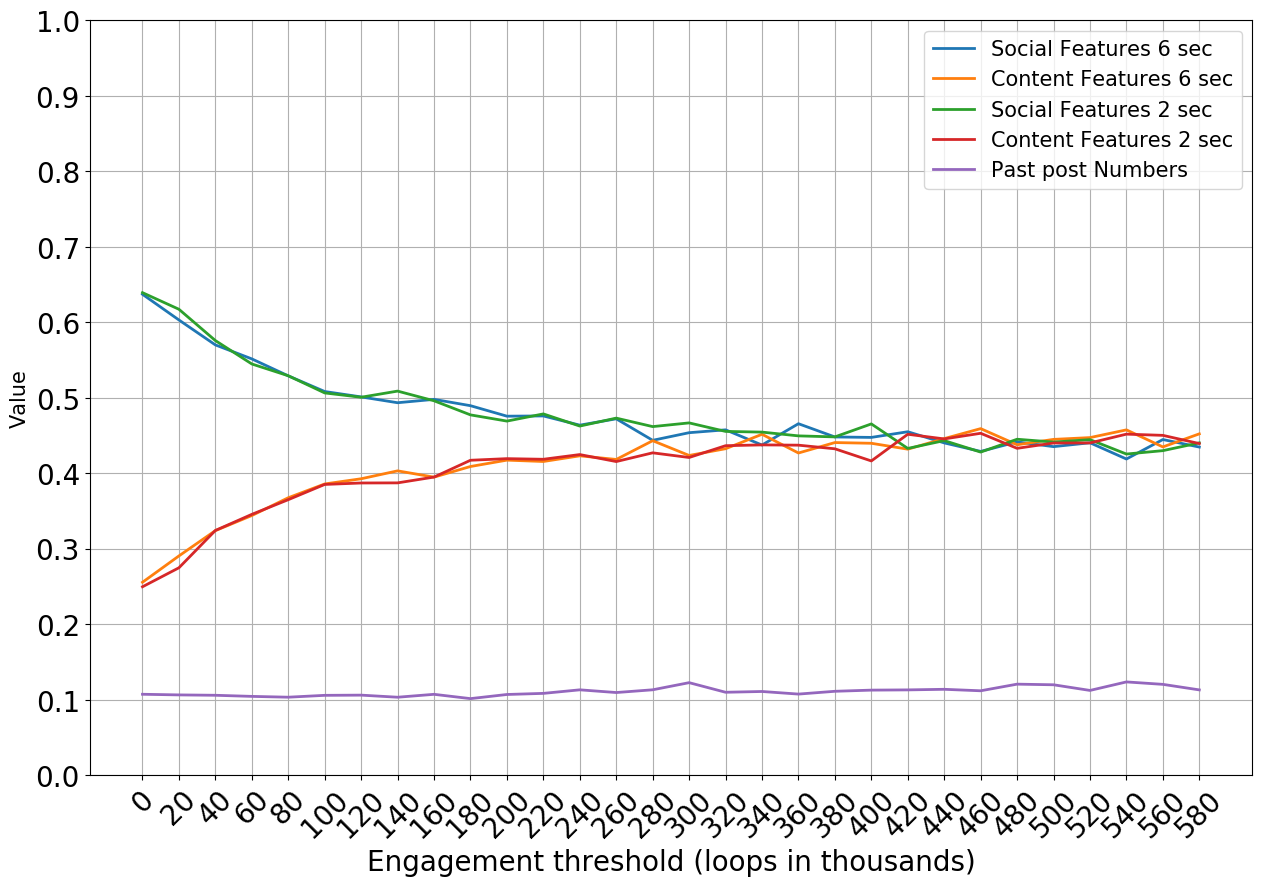
\includegraphics[width=0.5\textwidth, height = 4.5cm ]{engagement}
        \label{fig:Feature_importance}
    }
    \subfloat[ Individual Content Features ]{
        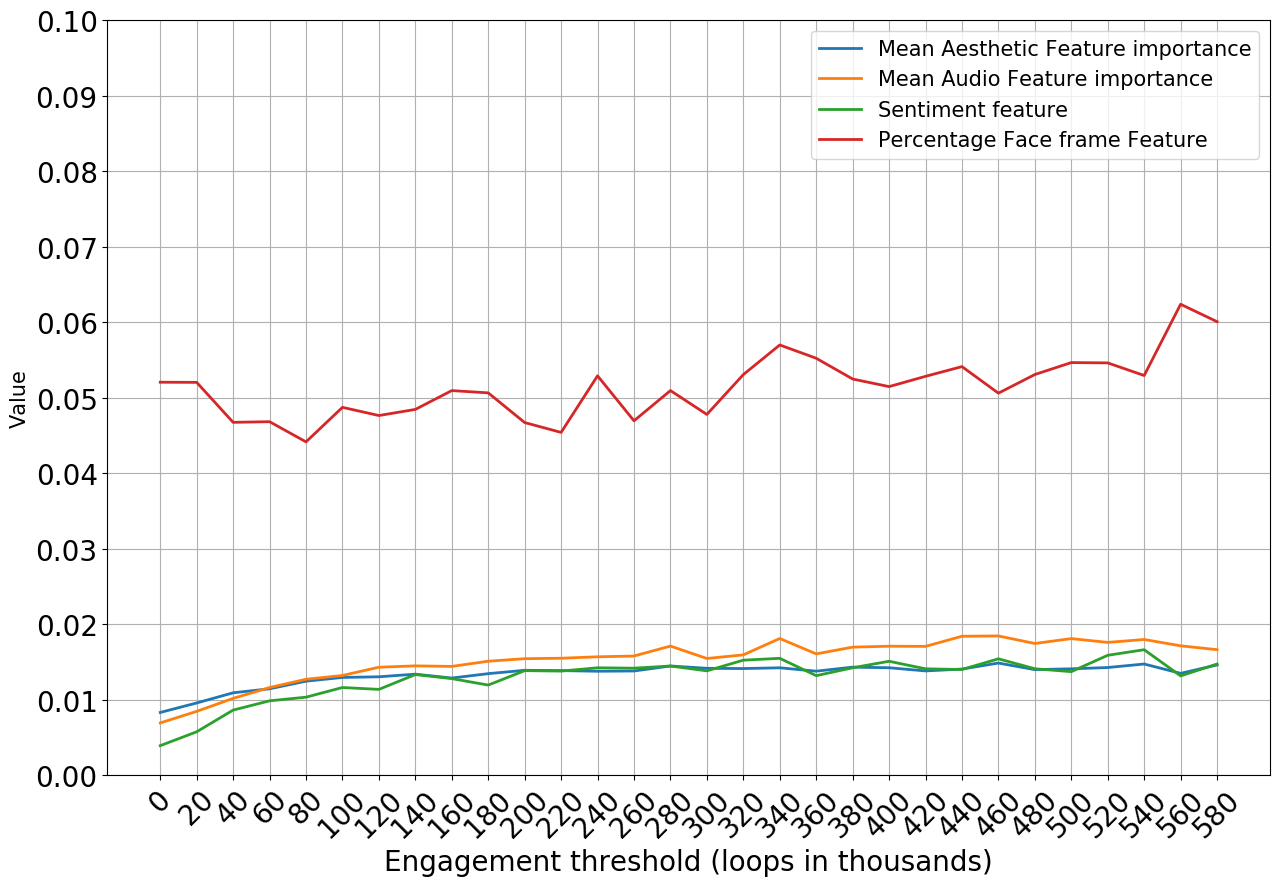
\includegraphics[width=0.5\textwidth, height = 4.5cm]{contentFeatures}
        \label{fig:Feature_importance_content}
    }
    
    \subfloat[ Classifier Performance ]{
        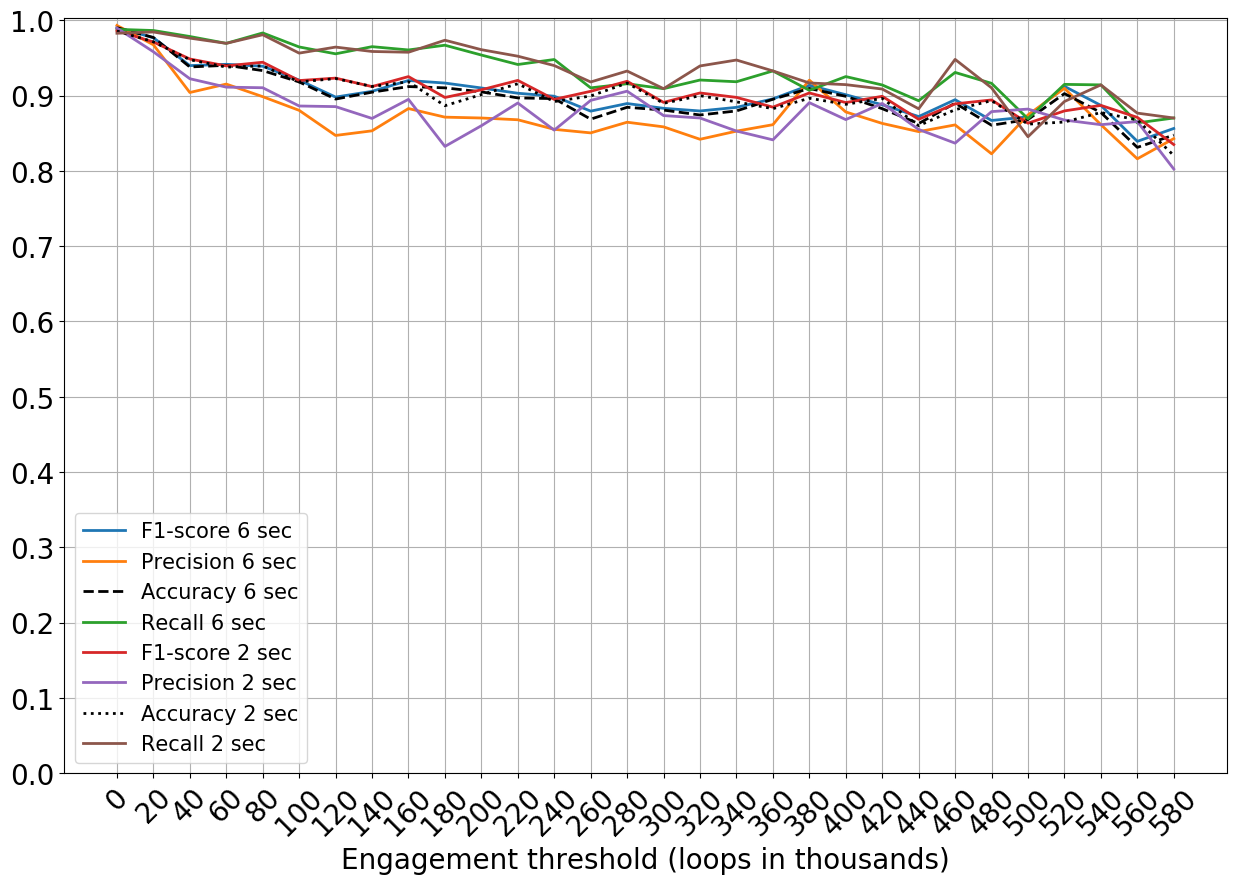
\includegraphics[width=0.5\textwidth, height = 4.5cm]{classifier_accuracy}
        \label{fig:Classifier_performance}
    }
    \caption{ Understanding engagement for different thresholds (min.\ number of loops considered as engaging). Two different classifiers are used, one using quality of the entire micro video (labeled 6 sec), the second measuring quality from only the first two seconds (labeled 2 sec). (a) As threshold becomes higher, content-related factors become as important as social factors (both classifiers). Note that unlike content quality computed from the first 2 seconds (`Content features 2 sec') rather than the entire 6 seconds of the video (`Content features 6 sec'), `social features 6 sec' uses the same feature values as Social Features 2 sec', but the two are plotted separately to show the relative  importance of social features in the 6 second vs 2 second classifier. (b) Amongst content features alone, presence of faces in the video is the single most dominant feature, across all threshold levels (6 second classifier) (c) Both 2 sec and 6 sec classifiers perform similarly across all metrics such as Precision, Recall and F1-score. Performance is high across all engagement thresholds: all metrics are consistently over 0.8 or 0.9.}
    \label{fig:classifier}
\end{figure*}




\begin{figure}[!htb]
    \centering
    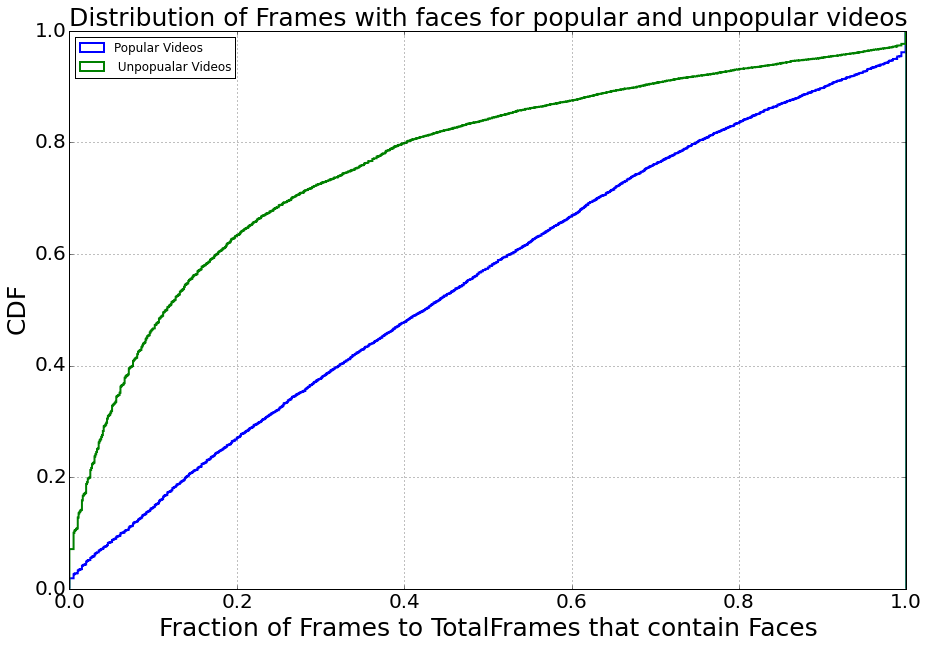
\includegraphics[width=0.6\columnwidth]{FaceCDF}
    \caption{\textsl{ CDF for popular and unpopular videos. The CDF signifies the cumulative distribution of percentages of frames containing faces in a vine video. The observation here is popular videos tend to have higher face percentage than unpopular videos}}
    \label{fig:Face_CDF}
\end{figure}


\section{Primacy of the first seconds}

%Our main observations so far are: \one\ \textbf{RQ1:}Vine micro videos appear to be different from both images (Flickr) and videos (YouTube) and \two\   \textbf{RQw:} content quality features, especially image-related ones (e.g., fraction of faces with frames) become  important for user engagement and popularity metrics. %and \three\ unlike videos where affect (sentiment) plays an important role in user engagement~\cite{bardzell2009understanding,fontanini2016web,eckler2011spreading}\footnote{See also {http://67.222.24.243/wp-content/uploads/2009/03/affect-study-screen-view.pdf} (accessed 24 Oct 2016).}, sentiments conveyed in the video appear to be much less important in Vine. 
Next, we try to understand these findings further by examining the quality of the individual frames of the videos: One way to think about videos is as a sequence of images. With micro videos, this sequence is of course much shorter than in other videos, and we investigate whether this has impact on video quality (\textbf{RQ2}). Our results show a ``primacy of the first seconds'' effect, with quality deteriorating over time and the quality at the beginning is as good a predictor of engagement as quality of the entire video.

\subsection{Image quality deteriorates over time}




Vine videos can be at most 6.5 seconds long. We sample the videos twice every second and represent the whole video as a series of 12-13 static frames. This sampling rate is not too low to miss any considerable frame transitions, neither is it too high to include a lot of mid transition frames. For each sampled frame, we calculate the feature under consideration -- sentiment, percentage of faces, and aesthetic score. To compute the aesthetic score, we extract the 18 aesthetic features described in Table~\ref{tab:Features_table}. for each frame frame. To find an aggregate overall aesthetic score of each frame, we use a weighted sum of all the features (This is possible because all the features are on the same scale), where the weights are calculated to be proportional to the importance of each feature in the classifier designed in the previous section. 


For each video and each feature, we then compute when in the video the feature reached its maximum value. We then divide the videos into two second intervals, essentially dividing the video into its first third, second third and third third. We then ask what proportion of videos had the maximum value of a feature in the first (respectively second and third) third. This procedure tells us when we are likely to find the `best' part of the video. 

\begin{figure}[!htb]
    \centering
    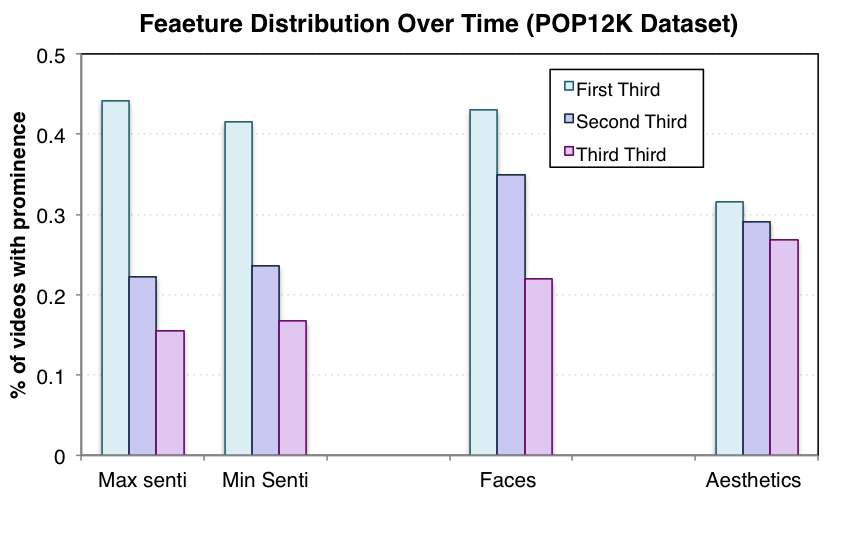
\includegraphics[width=0.7\columnwidth]{ThirdsDistribution.png}
    \caption{\textsl{Evolution of Feature magnitude: The graph shows sharp trend in prevalence of strongest component of a feature in the first one third of the video. The strength decreases progressively for the successive thirds. (Results shown for POP12K dataset. Similar results obtained for ALL120K.)}}
    \label{fig:Face_Thirds}
\end{figure}

Fig.~\ref{fig:Face_Thirds} shows the result for each major category of content-related feature, plotted over both our datasets (ALL120K and POP12K). We observe a general trend where the first third has the maximum (best) value for all features considered. For instance, the best aesthetic score is to be found in the first two seconds. Similarly, the proportion of faces, an important predictor of engagement (Fig.~\ref{fig:Face_CDF}), is also maximum in the first third. 

Note that for sentiment values, the minimum value is just as valid and valuable as the maximum, representing a sad or emotionally dark segment of the movie with negative sentiment, in contrast to a happy segment of the movie with positive sentiment. Therefore, we calculate which third of the movie we find the maximum and minimum sentiment values and plot these separately. In both cases, we find  yet again that the first third of the video has the maximum (minimum) sentiment value for the majority of videos. 

\subsection{Loops and likes are obtained on first sight: Initial seconds predict engagement}
\label{sec:first-seconds}
Collectively, the results above paint a picture where the first seconds of the micro video are highly important in engaging the user. We conjecture that this might be because of the mobile-first nature of Vine: the primary user interface is the Vine app, where users select which videos to watch by scrolling over it. The vine only plays when the user retains focus over the video, and hence the first seconds are likely critical for grabbing user attention and engaging them. 

We next take this result to its logical conclusion, and ask how the classifier developed in the previous section for predicting engagement would work if using only content-related features from the first third of the video rather than from the whole micro video. Following the same methodology as described in the previous sub-section, we develop a series of classifiers for different popularity thresholds, training this time on image content-related features drawn from the first two seconds of the video rather than from across the whole video. The same set of hyper parameters were used as in the previous setting. As shown in Fig.~\ref{fig:Classifier_performance}, the resulting classifiers (labeled 2 sec) perform very similarly to the classifiers developed before (labeled 6 sec). Further, Fig.~\ref{fig:Feature_importance} shows that the relative importance of different features is also nearly identical to the previous results. It should be emphasized that although these results were obtained using loop counts as the metric for user engagement, similar results have also been obtained using reposts (re-vines). 

These results point to a \emph{primacy of the first seconds} effect, whereby the first seconds of a micro video matter as much as the whole video, suggesting that they behave almost like still images in terms of user engagement.


\section{User study}
\label{sec:userstudy}
To complement the data analysis and gain deeper insight into what drives user actions and engagement, we designed an anonymous user study
which captures user behavior when engaging with micro-videos. 

\subsection{Survey methodology}
We initially recruited undergraduate students, obtaining about 33 responses.
Subsequently, we tweeted the survey out to the Official Vine Twitter account and to the accounts of Vine and Instagram users, in order to gain further exposure amongst 
users of these platforms. In all, 115 users responded to our survey. Table \ref{tbl:survey} summarizes the respondents' demography and usage preferences. Most questions asked were to be answered either on a 5-point Likert scale  (Strongly agree to Strongly Disagree), and or in a semantic differential format, with three options to choose from. 
%\footnote{Survey can be found here :  https://goo.gl/forms/lHEea9EzYCyRy3jQ2}.

\begin{table}[hbt]
    \centering
    \begin{tabular}{l|c}
        \thead{Attribute} & \thead{\shortstack{Value}} \\
        \hline
        Male respondents (\%) & 44.2 \\
        Female respondents (\%) & 55.8  \\
        \hline
        Age Demography (\%) &\\
        \hline
        18-24 & 43.4 \\
        25-31 & 34.5 \\
        32-40 & 14.2 \\
        40+    & 8 \\
        \hline
        %		Platforms used (\%) &\\
        %		\hline
        %		Instagram & 67.3 \\
        %		Snapchat stories & 27.4 \\
        %		%Whatsapp stories & 97 \\
        %		Vine & 2 \\
        %		\hline
    \end{tabular}
    \caption{Summary of survey responses}
    \label{tbl:survey}
\end{table}


%We asked users to select the micro-video platforms which the users are most exposed to. Snapchat and Instagram polled highest in the sample population.
%Although Vine polled  low in terms of declared usage, the reason being that Vine was declared to be discontinued as of the date when the survey was conducted\footnote{Moreover our survey was primarily answered by respondents from Europe and Asia, where vine had very limited penetration.}, almost 70\% of users declared to have used Instagram %which also hosts 
%micro videos. Hence this survey can be considered to be a good proxy for understanding ground truth user engagement with micro-videos. 

\subsection{Validation of data-driven results}
To understand engagement with micro-videos and validate the findings that emerged from our analysis of \textbf{RQ1} and \textbf{RQ2}, the survey asked the following 5 questions
to be answered on a 5 level Likert scale (strongly agree - strongly disagree):
\begin{enumerate}
    \small 
    \item [A] I tend to like/comment on videos from friends rather than from strangers
    \item [B] I always form an opinion of a video in the initial few seconds, once the video starts playing
    \item [C] I rarely watch short videos (Snapchats, stories) , all the way to the end.
    %\item [D] I don't really care about the quality of the micro-video or stories, as long as I like the content
    \item [D] I prefer to watch short videos of humans on these platforms. E.g.\ I like to see a person talking/expressing rather than outdoor scenery, or Cats.
\end{enumerate}

Almost 66\% users agreed to question \textbf{A}, which reaffirms the tendency of socially embedded users being able to get high engagement scores. 44\% of users agreed to question \textbf{B} (and further $\approx$ 30\% users were neutral) and 38\% users agreed with statement \textbf{C}, supporting the observed the ``primacy of the first seconds'' effect.
%55\% users agreed to statement \textbf{D}, suggesting a possible reason why . 
Contrary to our findings regarding faces, only 34\% users agreed with statement  \textbf{D} (although a further 39\% remained neutral; thus only a minority 27\% of users disagreed or disagreed strongly). Such result might suggest that for many users, our attraction towards face shapes is innate \cite{slater1998innate} and people do not consciously engage more with faces. %While further study is required to confirm this conjecture, we find that on a sample of 6000 Instagram micro videos, the top 10 percent of videos by popularity had 

\subsection{Understanding what matters to users}
The next part of the survey went beyond confirming the data-driven analysis by asking the respondents how their behaviour changed when it comes to \emph{acting} on a video they engaged with, i.e., when do they like/forward, comment or stop playing the video? 44\% like, comment or share videos only after finishing watching it, and but a sizeable 56\% agreed that they do so in the middle of watching the video itself, or right at the beginning (19\% share at the beginning. 37\% somewhere in the middle); again pointing to the need for capturing users in the initial parts of the video. 

Interestingly, a majority of 55\% of respondents agreed (on a 5 point Likert scale) to the statement: ``I don't really care about the quality of the micro-video or stories, as long as I like the content''. This result, together with the previous answers seems to imply that   the fall off in content quality in the latter parts of micro videos does not negatively impact user engagement. However, users do see a difference between micro videos and ``traditional'' (and older) user generated content platforms such as YouTube: an overwhelming 75\% of respondents rate the production quality of YouTube videos quality as more professional than micro videos.

\section{Discussion and conclusions}
In this work, we took a first look at user engagement with micro videos. Defining engagement in terms of social attention metrics such as likes, revines (reposts) and loop counts, we find that content quality-related features have as strong an influence as social network-based exposure in driving these metrics. Furthermore, the quality of the first couple of seconds is higher than the quality of subsequent seconds, and can predict whether a micro video will be engaging or not, just as well as looking at the quality of the entire video. We further conduct a user study to understand ground-truth user behavior when it comes to micro-videos. The study suggests that users tend to make quick opinions regarding micro-videos and engage with them almost in an image-like fashion, where they may begin but not finish  watching the short 5-10 second long video. 
%This `primacy of the first seconds' effect suggests the observation that  micro videos are somewhat closer to user-generated images rather than user-generated videos, which we corroborated by comparing popular micro videos on Vine  to popular images on Flickr and viral videos on YouTube.
On a big picture scale, we show that attention budgets are quantifiable if we have a large enough user engagement data. Drawing back to the DIKW pyramid, the wisdom gathered from this knowledge extraction pipeline can imply several things.
\begin{enumerate}
    \item Advertisements on the Web are driven by social attention metrics. Therefore advertisers need to know and adjust their strategies based on the insight that user attention is driven to a large extent by the initial seconds. Although  video ads do not appear to be common in today's micro videos, how to place ads that grab user attention within a short duration of time will be a problem that is interesting both from a research and a business perspective. 
    \item A possible reason for the deterioration of image quality is that it may be difficult to maintain image composition, focus etc using a mobile phone camera with moving subjects. Novel UI and multimedia techniques that can help correct for such quality deterioration could greatly help micro video creators -- and also represent a second promising direction for further study. 
    \item Recently, several micro video platforms have started extending the duration of micro videos. Although the wisdom of longer micro videos without appropriate editing tools has been questioned\footnote{\scriptsize http://www.theverge.com/2013/6/20/4448906/video-on-instagram-hands-on-photos-and-video}, from a research perspective it would be interesting to study how user behavior and engagement changes as longer micro videos become more common place. Interestingly, we find that in a small sample of about 6000 Instagram videos (where the maximum permitted duration is 60 seconds), users continue to prefer shorter videos, with 70\% of videos less than 20 seconds long, and the median duration at just under 15 seconds. Such user preferences can and should be considered as the micro video format evolves further on different platforms.
\end{enumerate}

More generally, in this work we considered user engagement as a single dimension of perception driven process. We acknowledge that user engagement is a very subjective notion, impacted by different factors including user location, habits, gender, visual preferences. In  future work, we plan to explore how such different user sub-cultures perceive and engage with micro videos, following recent works from the Multimedia community studying the impact of culture in subjective image perception \cite{jou2015visual}.









%______________________________________________
\chapter{Background}  %Title of the First Chapter 
\label{chap:background}

\begin{quote}
\textsl{If I have seen further it is by standing on the shoulders of Giants.} - Isaac Newton
\end{quote}

Studying signals in user interaction data, where the interactions are  driven by affective triggers, has been an active topic of research~\cite{picard2003affective,pantic2007human,cambria2012sentic,adibuzzaman2013situ}. 
As such it is worth discussing the different aspects in which the community of researchers have explored this area. The key aspects in which I would like to place my work is in terms of quantification of the subjective signals from data that originates from web scale applications. 
The two case studies in this dissertation attempt to quantify two distinct subjective properties, viz 1) Social support and 2) Aesthetic perception.
Here we would try to first, explore the definitions of the concepts of social support and Aesthetic perception, and then examine the literature for methods, models and metrics.

\section{Part 1: From communities}
There has been a surge in the number of online communities, since the rapid adoption of social networks across the internet. The spectrum of types and applications of these communities is as abundant as the possible subjects discussed on the internet. 
These communities have become a dedicated space for online users to discuss about topical items. Often these communities take the shape of a forum, where topical threads are started by an original poster (OP) and a discussion commences on this post. The discussions could be in the form of a debate\footnote{\url{www.kialo.com}}, a banter\footnote{\url{www.reddit.com}} or a peer to peer topical discussion\footnote{\url{https://healthunlocked.com/blf}}. In this dissertation, we aim to understand the nature of social support and the signatures of social support which can be quantified from these online spaces. To that end we aim to look at forums which have been self certified to be dedicated for hosting supportive discussions.

\subsection{Online social support}
According to Shumaker et.al~\cite{shumaker1984toward} social support is defined as "an exchange of resources between two individuals perceived by the provider or the recipient to be intended to enhance the well‐being of the recipient."
A lot of work has been done in understanding how social support functions and influences people in distress in the offline world. For example, a meta review~\cite{dimatteo2004social} showed that adherence to a medical treatment is 1.74 times higher, if the patient hails from a cohesive family structure. Social support has also shown to be a crucial factor in the positive prognosis of patients suffering from chronic and long term conditions~\cite{sacco2006diabetes,peirce2000longitudinal,brown1986social,collins1993social,dunkel1984social,baron1990social}. All this literature evaluates social support from a psychological stand point, in that, it looks at how a patient/subject is perceiving support from its real world network (family, friends, doctors etc.) More over most of this work uses the qualitative frameworks and tools as a way to measure off-line social support. 

Social support, or the perception of help received from others, is a widely studied as a psychological resource used to cope with distress. 
Social support is generally classified into one of the following categories viz. Informational, Tangible , Network or Emotional~\cite{cutrona1992controllability}. These categories measure the nature of social support along the idea of exchange of resources between the person in distress and the one providing support. For example, an informational support could involve pure exchange of valuable information about dealing with an issue. Whereas as network support could purely allow the recipient to acquire a wider network of people through the support giver or a support platform (think societies like Alcoholic Anonymous). 

The online world is very good at filling the gaps where offline support groups may fail. That is, the online groups, if designed in the right way, could provide essential informational, network, and at times emotional support at the click of a button. The internet makes both information and user networks, easily accessible. The utility of such spaces can be believed because of the evidence such as: online support groups being associated with quality of life~\cite{idriss2009role,nambisan2011information,coulson2005receiving}, improved control over additions~\cite{wood2009evaluation}, improved triaging with suicide ideation~\cite{languageChoudhury} and mental health issues~\cite{kummervold2002social}. 

Despite the interesting evidence, the common theme in most of these works is that they all take either a qualitative approach to understanding online support, or a language driven approach~\cite{de2014medical,de2016stroke,de2017adolescents}.
Most methodologies either utilize expert knowledge to dissect what is being said on these forums, or a natural language approach to understand the key language patterns on these forums. Either ways, the key missing bit in this picture is understanding how and where do the individual users fit in. How do they help in keeping the entire support community functioning. More over, we do not have any understanding about the structure of a supportive conversation online from the perspective of a user in distress. This is especially interesting, since there are obvious offline markers of a supportive conversation, whether it being a group, or a peer to peer setting. Not just that, but there are several therapy strategies like Communication accommodation~\cite{coupland1988introduction} or group psychotherapy~\cite{yalom_theory_1995}. So it is worth investigating these aspects of online support communities.

For this exact reason, \textbf{RQ1, RQ2 and RQ3} would make progress towards understanding the dynamics, local and global structures of online support communities.
 
\subsection{Social networks, support, and metrics}
Modelling and studying online social networks, through the lens of complex network theory and network physics has been an active area of research since the 1980s. The idea of looking at (offline) social structures as social networks was quite prominent in the fields of sociology~\cite{scott1988social}, but the most important leap in this field came with the advent of online social networks. This opened up new doors in measuring and understanding how humans form networks, and do so at scale through the medium of online networks~\cite{mislove2007measurement}. The first of these works~\cite{mislove2007measurement} explored the idea of looking at large scale user graphs to measure and evaluate a lot big picture attributes about online social networks. In that, they measure the long tailed nature of social links, the symmetric nature of social links and the overall sizes of connected components.
A connected component in a social graph $G(V,E)$ ) -- where $V$ are the vertices or users and $E$ are the edges between them -- is a set of nodes $\{C\}$ where all nodes $\{c_i \in C\}$ have connected paths to all other nodes in $\{C\}$. The size of the largest connected component was often used as a proxy for the connectedness of a social graph~\cite{myers2014information,traud2012social,woodhouse1994mapping}.
Other global scale metrics explored for understanding social networks were degree distributions~\cite{muchnik2013origins,newman2002random, kossinets2006empirical}, clustering coefficient ~\cite{opsahl2013triadic, toivonen2006model} and centrality~\cite{opsahl2010node, borgatti2009network}. All these metrics aim to look at how nodes(users) in a social graph group together or how do they interact with each other as the size of the network increases. 
These insights help network physicists model how information or a contagion diffuses in a connected community. However , despite the large number of interesting works that look at network structure, there have been limited progress in using these tools to understand the nature of social support in online networks.

In the offline world, there have been some studies that look at the ego network of a person of interest, to infer the nature of social ties they have. In that, they look at the transitive nature of social networks around a person~\cite{golden2009social,doi:10.1177/104649647100200201, lin2001social}. This means, how many friends of a person, are friends among themselves. A completion of this triad -- which implies that friends of my friends are my friends -- is called a triadic closure.
In the online world, the theory of social capital and triadic closures were operationalized in terms of triadic census~\cite{faust20077,faust2008triadic}. The census simply profiles any given network by counting individual instances of the individual sub-graphs made of two, three, or in some cases four nodes. These sub-graphs are called motifs.
The importance of triadic motifs in social network research has been stressed so much so that in the words of  Holland and Leinhardt~\cite{holland1977method} 
\begin{quote}
    ``The essential issue of any notion of structure is how the components are combined, not the components themselves...this issue amounts to the proposition that the lowest interesting level of structure...is the level of triples of nodes—the triadic level''
\end{quote}


From the studies discussed here, the link between human to human interactions and their emergent network structure are quite evident. For this reason it is natural to extend this link to explore how perceived social support manifests in these interactions. In this dissertation, I aim to first quantify how network structures in support communities evolve, and second, discover the signature structural properties of these interactions over support communities.

\section{Part 2: From crowds}
The second part of the dissertation explores new methods to use crowd's opinions, in order to build models of our subjective perception of urban spaces. The idea of using crowd based annotations or opinion mining has been popular and has been exploited in the recommendation systems literature for a while. Here I would introduce some background about the idea of crowd sourcing, how it applies to quantifying the subjective, and how it has been used to understand urban spaces and cities. 

\subsection{Crowd sourcing and the subjective}
Crowdsourcing has been an important part of the computer science research for the past decade. The idea of crowdsourcing was first brought to attention by Jeff Howe~\cite{howe2006rise}, where he introduced the idea of a logical equivalent of outsourcing -- which is sending the jobs outside an area, where labour prices are competitive-- but for more transactional and atomic tasks. This idea was quickly adopted by the academic community, right after the inception of services like Amazon Mechanical Turk or Crowdflower~\cite{paolacci2010running}.

The natural extension of this new method was to use it for annotating large quantities of data. These annotations generally dealt with labels of objective nature, such as objects~\cite{vondrick2013efficiently}, relationships between objects~\cite{krishna2017visual}, or annotating textual data like named entities~\cite{finin2010annotating}.

The key idea behind crowdsourcing is to get a cognitive input about unlabelled data by incorporating opinions of hundreds of ``crowd-workers'' exchange for money. This is done in order to annotate the data with the most accurate objective labels, that come from a human annotator. This data then becomes the training set for a downstream machine learning algorithm . These algorithms would then learn the task of classifying unseen data into their respective correct labels. 

But the very fact that a cognitive process is at the root of the annotations implies that this framework can even be applied to subjective properties, provided that the annotators can arrive at a consensus, and we have large enough samples. The most appropriate use case is that of annotating expressions or affects of humans in videos or images. Despite the subjective nature of perceived affect, most neuro-typical humans tend to agree on what constitutes the expression of anger, sadness, happiness , disgust etc. In that spirit, several studies~\cite{tavares2016crowdsourcing,katsimerou2016crowdsourcing,kim2016vinereactor} tried to build machine learning models that could detect emotions from facial expressions, using data annotated by the crowd.

Apart from building a model of human affects from faces, crowdsourcing was also applied to the area of quantifying the actual affective stimuli in content. That is it tries to quantify the intangible property of a content that stimulates evocation of a particular emotion in the consumer of that content. For example, it is worth asking ``Which emotion does an image of a sunset evoke in the human seeing it?''. This question goes one level deeper by trying to quantify that which evokes positive or negative sentiments. To that end Sentibank~\cite{SentiBank} explored this idea by training a deep learning model on Flicker images which were annotated for evoking positive or negative sentiments. The same team extended it to analyse how the evoked emotion changes as a function of culture and language~\cite{pappas2016multilingual}. Indeed they found that these evoked emotions are also dependent on the language, culture, and other social properties of the annotator. Although these works exposed some limitations in the approach of quantifying the subjective, they also showed that by and large, these techniques work if the data is large enough and there is considerable consensus among the annotators on the topic of the annotated subjective property of the data.


\subsection{Crowds and the cities}
So far, the most detailed studies for quantifying the perceptions of urban environments and their visual appearance have relied on personal interviews and the observation of city streets: for example, some researchers relied on annotations of video recordings by experts~\cite{sampson04seeing}, while others have used participant ratings of simulated (rather than existing) street scenes~\cite{lindal2012}. 
But since the advent of services like the Google street view and Open Street Map, the Web has now been used to survey a large number of individuals. Place Pulse is a website that asks a series of binary perception questions (such as `Which place looks safer [between the two]?') across a large number of geo-tagged images~\cite{salesses2013collaborative}. In a similar way, Quercia \emph{et al.} collected pairwise judgments about the extent to which urban scenes are considered quiet, beautiful and happy~\cite{quercia2014aesthetic} to then recommend pleasant paths in the city~\cite{quercia2014shortest}. Another study~\cite{seresinhe2015quantifying} presented the annotators with a 10 point scale, which they would use to score a place(Street view) for its aesthetic beauty. 
All these studies relied on the crowds, in that the annotators were completely disconnected from each other, and their ratings were purely based on their exposure to the image or an urban scene. An important caveat here, as in case of multi lingual sentibank~\cite{pappas2016multilingual}, is that the cultural and social background of the annotator would play a role in how they perceive an urban scene.
But on average, these annotations proved very useful in understanding something as subjective as the perception of safety, beauty, or memorability in urban spaces. 

This can be indicated by the fact that lately deep learning techniques have been used to accurately predict urban beauty~\cite{dubey2016deep,seresinhe2017using}, urban change~\cite{naik2017computer}, and even crime~\cite{DeNadai16,arietta2014city}.  Recent works have also showed the utility of deep learning techniques in predicting house prices from urban frontages~\cite{frontage}, and from a combination of satellite data and street view images~\cite{law2019take}.

All the studies discussed above were successful in quantifying the subjective properties of an urban scene using predictive machine learning models. But there is a significant gap between predicting and explaining the prediction in order to guide interventions. This explainability problem is prevalent in almost all applied machine learning system. In this dissertation, I attempt to make some progress on the front of explaining the reasons behind perceiving an urban scene beautiful or ugly. These explanations also come in the form of urban design metrics, which can guide interventions from the practitioners of this field.

\section{Discussion}

The title of my dissertation enumerates the two regimes --communities and crowds-- under which I explore the problem of capturing the signatures of perceived subjective properties, using customized metrics and models. The over arching thesis has always been understanding how human perceptions guide our actions on the web scale, and how these actions leave behind traces of the subjective triggers.

In the following chapters, I will discuss the different methods, metrics, and models that are developed in order to make progress in answering the central thesis of this dissertation.



%*******************************************************************************
%****************************** Second Chapter *********************************
%*******************************************************************************

\chapter{From communities: The actors of online support }

\label{chap:Utility_support}
\graphicspath{{Chapter2/plots/} {Chapter2/plots}}
\begin{quote}
    \textit{''The original idea of the web was that it should be a collaborative space where you can communicate through sharing information... In an extreme view, the world can be seen as only connections, nothing else.``} - Tim Berners Lee\cite{berners2001weaving} 
\end{quote}
Attention budgets pretty much govern how we as consumers interact with online social networks. It has been shown that the dearth of this budget, promotes an engagement behaviour that prioritizes perceptive features and immediacy in the content~\cite{joglekar2017like}. The scrollable user interfaces of platforms like Instagram and Facebook, allow mere seconds to decide whether a particular content is worth the user's attention~\cite{eikelboom2017irresistible}. 

However, there is a whole breed of online social networks, which aim at bringing the offline sense of networking, online. These networks are mostly designed around a specific purpose like technical discussions\footnote{\url{www.stackoverflow.com}}, subject specific questions\footnote{\url{www.stackexchange.com}} or simply around hobbies like knitting\footnote{\url{www.ravelry.com}} or art\footnote{\url{www.artween.com/}}. These communities embody the true essence~\cite{berners2001weaving} of the internet, in that they strive at making geographical distance secondary, to the act of social networking and information sharing.

\section{Introduction to online social support}

According to the seminal work by Shumaker and Browne ~\cite{shumaker1984toward}, social support is defined as \textsl{``an exchange of resources between two individuals perceived by the provider or the recipient to be intended to enhance the well-being of the recipient.''}. In the context of online spaces, the definition prescribes exchange of messages and information, in order to provide support to the recipient.  

This exchange has been explored in detail in the field of computer mediated support~\cite{coulson2005receiving,weinberg1995computer}. The main idea of understanding computer mediated communication is to zoom out from the message level interactions between users, and look at the actual ``tie'' between them. A tie connects a pair of actors by one or more relations. Pairs may maintain a tie based on one relation only, or they may maintain a multiplex tie, based on many relations, such as sharing information, giving financial or psychological support~\cite{garton1997studying}. Thus ties also vary in content, direction and strength. Ties are often referred to as weak or strong, although the definition of what is weak or strong may vary in particular contexts~\cite{marsden1984measuring}. 

A lot of qualitative work has been done on understanding the dynamics~\cite{wright2003health,languageChoudhury} and utility~\cite{nambisan2011information} of online social support. But most, if not all, studies looked at the content and thematic aspects of the supportive posts on these forums. But the key strength of online support communities is their networked collection of users, volunteering to provide online support. Some examples of such communities are  r/SuicideWatch\footnote{\url{www.reddit.com/r/suicidewatch}}, r/Depression\footnote{\url{www.reddit.com/r/depression}}, Elefriends~\footnote{\url{https://www.elefriends.org.uk/}}. These communities are apt Petri dishes to study the structural signatures of the online social support networks. Once you could quantify the social support signatures in terms of computable metrics, platforms could then empower the participants of these communities and design interventions to curb negative behaviour like trolling.

In the context of this dissertation, I wanted to know how signatures of a perceived entity like social support,  manifests on these formal social networks.
This resulted in a framework that uses a set of network metrics to measure the dynamics of support communities and the importance of individual actors for the health of this community. 

This framework could bear significant potential impact on the problem of measuring health and utility of online forums. 

\section{Primer on online health communities}
\label{sec:primer}
Recent work has proposed that online communities have the potential to influence health and health care sectors. Recent studies have suggested that the participation of people with long-term conditions (LTCs) in online communities (1) improves illness self-management~\cite{allen2016long}, (2) produces positive health-related outcomes\footnote{\url{https://bit.ly/2FLcs1F}}~\cite{mo2012developing,pendry2015individual} , (3) facilitates shared decision-making with health care professionals~\cite{bartlett2011investigation,izuka2017stroke}, and (4) may even reduce mortality~\cite{hobbs2016online}.

There is also evidence that self-management support interventions can reduce health service utilization~\cite{panagioti2014self,taylor2014rapid}. This is especially a crucial point as the world health services are facing the brunt of an ageing population.

Online communities have experienced an upsurge in popularity among people with chronic respiratory conditions such as cystic fibrosis~\cite{kirk2016exploration}, asthma~\cite{stewart2011online}, pulmonary hypertension~\cite{matura2013virtual} and chronic obstructive pulmonary disease (COPD)~\cite{wentzer2013narratives}. More than 15 million people in England suffer from a long-term condition or disability, and they account for at least 50 percent of all general practitioner appointments\footnote{\url{https://bit.ly/2EVFs9v}}. Thus, assessing how these online communities function, evolve and provide perceived support, can have important implications for health care sector. More so, understanding the dynamics of these online communities, have actual repercussions on how the platforms that host them, could become a better resource of self-management of LTCs.

On average, one in four people with an LTC who use the Internet tries to engage online with others with similar health-related concerns~\cite{fox2011social}. In particular, it has been suggested that the value of participating in an online community lies in the possibility of gaining access to a range of people and resources quickly, easily~\cite{armstrong2000real}, and anonymously~\cite{pendry2015individual}, as well as obtaining tailored information and emotional support~\cite{ali2015online,de2017adolescents,shoebotham2016therapeutic,coulson2005receiving,de2016stroke}. However, most of this evidence comes from qualitative studies, whereas only recent years have witnessed an increasing interest in quantitative assessments of online communities as intervention mechanisms. 

The potential future integration of online health support systems with formal health care provision should be underpinned by a better understanding of how they are used and by evidence of their effectiveness. Indeed, as suggested by the Medical Research Council~\cite{Craiga1655}, integrating online support systems with the more traditional health care provision would require the identification and comparative assessment of potential alternative intervention mechanisms.



With the clarity on the importance of online health forums for people suffering from LTCs, this chapter investigates the role of individual users and the inter-user exchanges in keeping an online health community functioning. We would like to know whether there are particular users who play crucial roles in the communities. What are some peculiar behaviours which differentiates users on support communities for others?

With this context, we aim to answer the \textbf{RQ1} and \textbf{RQ2}, which are: 

\noindent\fbox{\begin{minipage}[t][2\height][c]{\dimexpr\textwidth-2\fboxsep-2\fboxrule\relax}
        \textbf{RQ1} \textsl{What dynamics of support communities help them thrive?}   

        \textbf{RQ2} \textsl{What differentiates \textbf{users} on support communities from generic ones?}   
\end{minipage}}

\section{Dataset}
\label{sec:dataset}
This study was carried out in collaboration with HealthUnlocked\footnote{\url{http://www.webcitation.org/70Y10rppl}}, the online forum platform that hosts the Asthma UK and British Lung Foundation communities. The data was aggregated, anonymised, and shared after proper Institutional Review Board and ethics approvals were taken to protect user privacy. The data was collected from  registered users, who can choose to either write posts publicly or send private posts to one another. In the latter case, posts are shared between 2 users only, whereas when posts are written publicly, a large number of users can become connected through threads of posts. In this study, I do not consider private posts. 
A thread is a series of posts made on one root post (RP), as a response to the root, or as a response to one of the responses to the root. This tree-like structure of posts can evolve indefinitely between posters and responders. 
For this study, user identifiers (IDs) were anonymized by the HealthUnlocked platform, and no demographic information was collected. 
The dataset included posts and their metadata (ie, the anonymized user ID numbers), user roles (eg, user, administrator, or moderator), date of posting, the hierarchical level of the post within the corresponding thread, and the dates on which the users joined and left the community. A sample of one such post can be seen in table \ref{table:sample}. Both communities were moderated, and HealthUnlocked moderators (identified through metadata field "Role") were included in the analysis to assess their contribution and compare it with other users. Online communities on the HealthUnlocked platform benefit from additional functionalities compared to other online forums, such as built-in patient groups that moderate the content. In particular, the content accessed by users is tailored to their interests, and profiles highlight users’ condition, chosen community, medications and treatments they use or find interesting. No data were collected on participants’ characteristics, though only people declaring themselves to be older than 16 years were permitted to create an account and take part in the online communities. Table \ref{table:jmirData} summarizes the salient features of the dataset used for this work. 


\begin{table}[htb!]
\centering
\begin{tabular}{ |p{5cm}|p{5cm}|p{5cm}| }
    \hline
    \multicolumn{3}{|c|}{Dataset Properties} \\
    \hline
    \hline
     \textbf{Property} & \textbf{AsthmaUK} & \textbf{British Lung Foundation} \\
    \hline
    \hline
     Time span of data   	& 02/03/2006-06/09/2016    	& 13/04/2012-06/09/2016 \\
    \hline
     Total Time (weeks)  	& 548						& 230 \\
    \hline
     Total number of posts	& 32,780					& 875,151 \\
    \hline
     Percentage of posts with at-least 1 reply & 87.3\%			& 93.1 \% \\
    \hline
     Total number of users &	3345					& 19,837 \\
    \hline
     Users who contributed > 1 posts (\%n) & 722 (21.6)  & 6628 (33.4) \\
    \hline
     Users who contributed exactly 1 post(\%n) & 331 (9.8) & 1186 (6.0) \\
    \hline
     Registered users who never posted (ie, lurkers), n (\%) & 2292 (68.5) & 12,023 (60.6) \\
    \hline
     Number of posts per user, $\mu(\sigma)$ & 14.2 (55.0) & 66.9 (75.1) \\
    \hline
    Number of posts per users who posted >1, median (min - max) & 5.1 (2-1068) & 8.0 (2-8947) \\
    \hline 
    Number of posts per users who posted >1, mean (SD) & 20.4 (65.6) & 88.1 (458.6) \\
    \hline
    Posts contributed by top 1\% users by activity, n (\%) & 10,457 (31.9) & 426,198 (48.7) \\
    \hline 
    
    \hline
\end{tabular}
\caption{Salient statistics for the data acquired from AsthmaUK and BLF forums.}
\label{table:jmirData}
\end{table}

\begin{table}[htb!]
    \centering
    \begin{tabular}{ |p{5cm}|p{10cm}| }
        \hline
        \textbf{Field} & \textbf{Sample Value}\\
        \hline
        Body   	&  \textit{"5 years ago i was diagnosed with emphsyma asthma and copd after being rushed into intensive care.
        Since then ive had the inhalers and tablets but never really been able to talk to someone about my 
        experiance so any help or advice would be very much apprieciated i have felt very lonely and frustrated 
        at times with this complaint as getting used to not being able to do what i could is the worst part.
        I am 58 and always thought i knew about life but im lost with this.
        It seems my life is all about thinking of how i am going to be feeling when i get up in a morning."}  \\
        \hline
        AuthorId & VVpb (anonymised) \\
        \hline
        Title & \textit{"What is breathe easy?And any advice on copd please"} \\
        \hline
        SuperRecipientAction & "N/A" \\
        \hline
        Action & Level 0 post \\
        \hline
        ThreadId & q5XXV \\
        \hline
        Date & 2012-06-09 09:53:15 \\
        \hline
        PostId & q5XXV \\
        \hline
        Recipient & N/A\\
        \hline
        Role & N/A\\
        \hline
        
    \end{tabular}
\caption{An example of a record from Health unlocked British Lung Foundation forum. The fields describe meta data about the post, such as timestamp, PostId, AuthorId etc. The data also contains the main body of the post as well as meta information about the conversation structure. In this case, the post is a root level post. Hence the recipient field is "N/A" and the Action field contains "Level 0 post".}
\label{table:sample}
\end{table}
        

The datasets span, respectively, 10 years for the Asthma UK and 4 years for the BLF communities (see Table ~\ref{table:jmirData}).

Despite the shorter time span, as a result of the larger number of users, the number of posts in the BLF community was higher than in Asthma UK, namely 875,151 compared to 32,780 respectively. Moreover, BLF users wrote a higher number of posts per user and were connected with a higher number of other users when compared with people in the Asthma UK forum (see Figure 2). In both communities, 60\%-70\% of registered users wrote no posts (ie, they were lurkers). Users who wrote more than one post contributed with a median of 8 (range 2-8947) and 5 (range 2-1068) posts in the BLF and Asthma UK communities, respectively.

The number of official moderators among the highly active users was negligible; there were no moderators in the top 5\% contributors to BLF and only 2 in the top 5\% for Asthma UK. Thus, our network analysis predominantly reflects content originated from registered users. This also means that moderators on these forums have more of an observatory role and do not engage in active support. 

When classified according to posting activity (ie, number of posts written to the forum), the top 5\% users contributed to a substantial proportion of all posts: 58\% and 79\% in the Asthma UK and BLF communities, respectively. In the context of this thesis, \textsl{Superusers} were those who made high number of connections (exchange of messages) with other users across the lifetime of the community.


\section{Graphs and their metrics}
\label{sec:graphs}
To understand the dynamics of these communities and their interaction structures, I convert the data from all the  exchanges of messages between users into graphs. In these graphs the users are represented by nodes and messages are represented by edges between users. 
More formally imagine a directed graph $G(V,E)$ involving a set of users $V_i\forall i \in N$ where N is the total number of users interacting on a health community. For every message exchanged between a user $i$ and a user $j$ we create an edge $E_{ij}$. By this method the complete community would form a global graph based off total interactions between all pairs of users, which we call a global graph $G_g$. Similarly we may decide to only consider the users which exchanged messages on one particular thread. Such a graph is called a thread graph $G_t$.

\begin{figure*}[!ht]
    \centering
    % \hspace*{-5mm}
    \subfloat[]{
        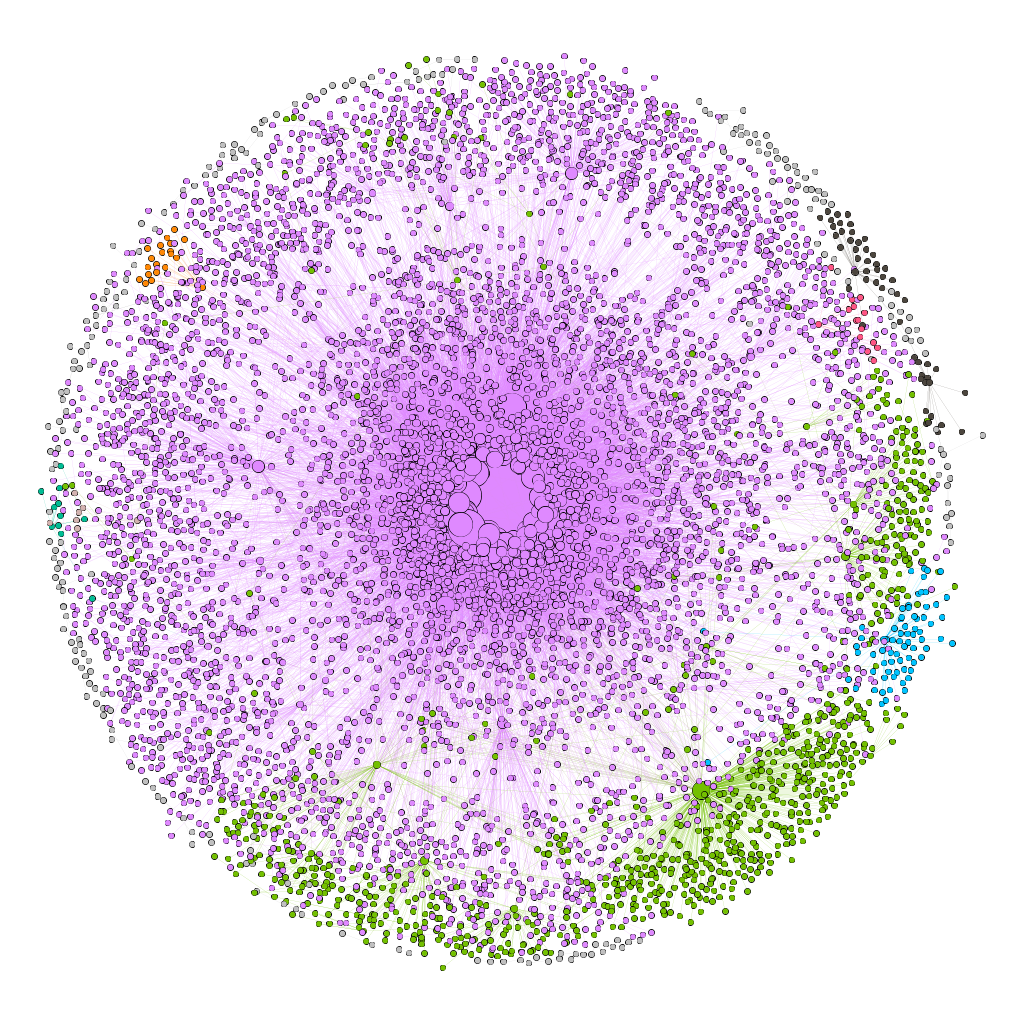
\includegraphics[width=0.5\textwidth ]{BLFWhole.png}
        \label{fig:BLF_graph}
    }
    \subfloat[]{
        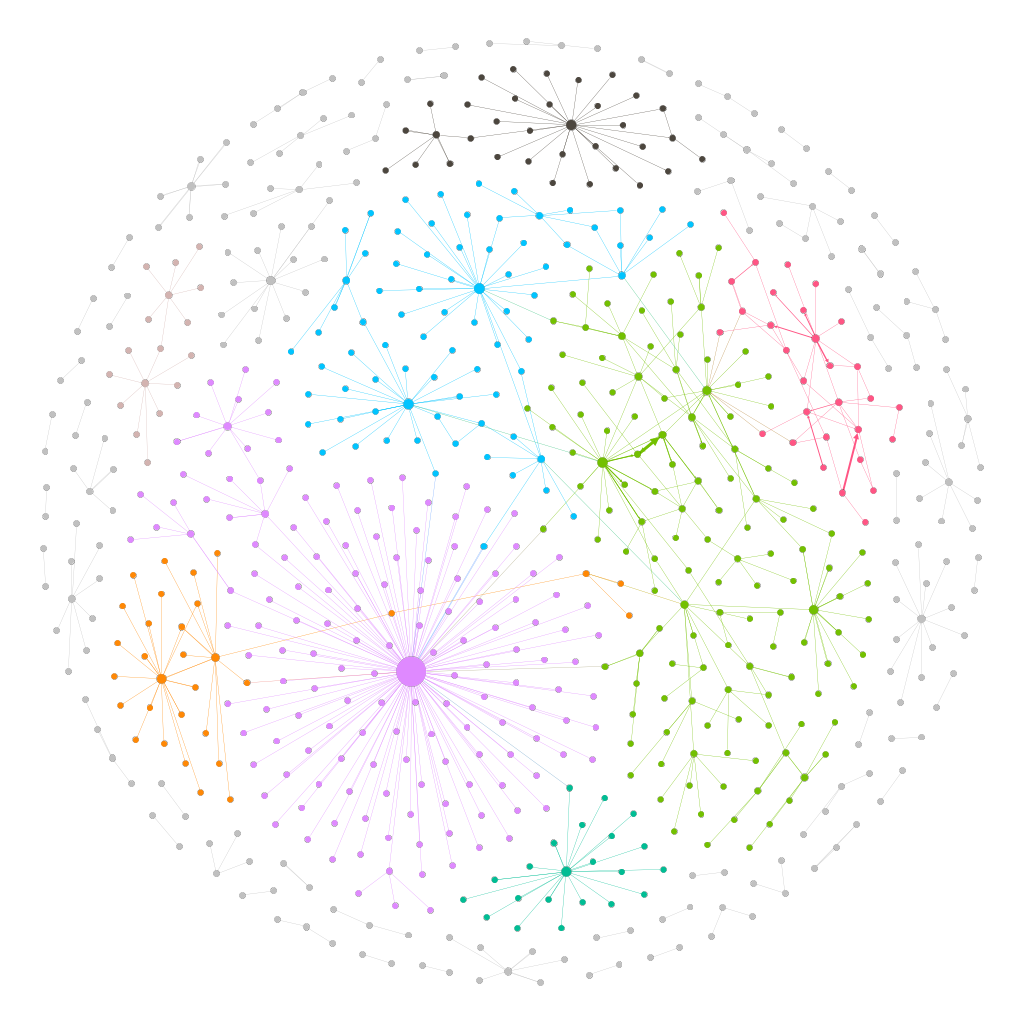
\includegraphics[width=0.5\linewidth ]{AsthamaWhole.png}
        \label{fig:Asthma_graph}
    }
    \caption{Global graphs prepared from Asthama UK community\ref{fig:Asthma_graph} and BLF community\ref{fig:BLF_graph}. The size of the node corresponds to the degree of the node and the color corresponds to the community membership }
\end{figure*}

These graphs abstractions ($G_g$ and $G_t$) represent the interaction structures which we intend to dissect. To understand the behaviour of these users, I evaluate several metrics on these graphs in order to understand the utility of these communities in terms of activity of sharing and support.

\subsubsection{Degree distributions and connectivity}
When you have a collection of nodes, connected to each other by edges, it is worth understanding how connected an average node is. More specifically, we would like to know the distribution of degrees, or the amount of edges a node has, across all the nodes in a graph. This metric is called the degree distribution of a graph, and it has been widely used in the complex networks literature as a measure to characterize types of graphs ~\cite{muchnik2013origins,ahn2007analysis,leskovec2008microscopic,raman2019challenges}.
We are specifically interested the nodes(users) who belong to the highest 1\% range of degrees. These users are the ones who are most interactive and have established edges with a lot of other users by exchanging messages. These users are called ``superusers''. 

\subsubsection{Largest connected component}
A largest connected component of a graph $G(V,E)$ )is the largest possible sub-graph $G_L(V_L,E_L)$ of $G$, such that each node in $G_L$ has at least one valid connected path to every other node in $G_L$. By evaluating the largest connected component on $G_g$, we can find the subset of users in the community which form a cohesive community. Furthermore, by measuring the effect of removal of certain ``superusers'' from this sub-graph on the overall size and structure on $G_L$, once can deduce the importance of the said users to the cohesiveness of a community. 
We can also measure the characteristics of the largest component on a temporal basis. By examining the fraction of users in a given week that belong to the largest connected component, one can estimate the focused and cohesive nature of interactions.


\subsubsection{Social capital and triadic closure} According to the literature, social capital is defined as those features of social structures, such as interpersonal trust and norms of reciprocity and mutual aid, which act as resources for individuals and facilitate collective action~\cite{collins1993social,coleman1988social}
It is common to quantify social capital in the context of social networks, by looking at structural holes, or unmet potential social links in the network. This is where ties between otherwise unconnected neighbours are filled in, sometimes called as closures, thereby benefiting the broker and the two neighbours by adding an extra link for information to diffuse. 
Such mechanisms have been studied in the sociology literature for decades. Work by Granovetter~\cite{granovetter1977strength} explored these structural holes and proposed that they are detrimental for efficient diffusion of information and resources in social networks. He also at times called these the ``forbidden triad'', referring to their propensity to close up in social networks. Such closures are, according to Ronald Burt~\cite{burt2004structural,burt2009structural}, necessary for information brokerage, and at times directly equate to social capital of these broker nodes.
In our case, as so much evidence has shown that the brokers of social support are often the superusers, we would certainly want to investigate how these users affect the cohesion and structural holes in the graph.


\section{How do support communities thrive ?}
To answer the \textbf{RQ1}, it is first worth asking how the user interactions bind the community together. We would like to know if the messaging activity is highly concentrated around a few sets of users or is it covering a large fraction of the user base. More so, it is worth asking if there are any special users who bear the mantle of providing support. This can be observed from the measured metrics of the interaction graph. 
From table\ref{table:jmirData}, it is evident that a minority of users are generating a bulk of data on these communities. E.g. the top 1\% users by activity contributed 32\% posts to AsthamaUK community. Such level of activity makes these users extremely important in understanding the dynamics of support on these communities. We term these users as ``Superusers''.
But before looking at the role of these superusers, it is first worth analysing the overall activity patterns on these communities. Do these communities drive enough engagement and activity to sustain them over long periods of time?  

\subsection{Temporal activity patterns}
\label{sec:activity}
\begin{figure}[!ht]
    \centering
    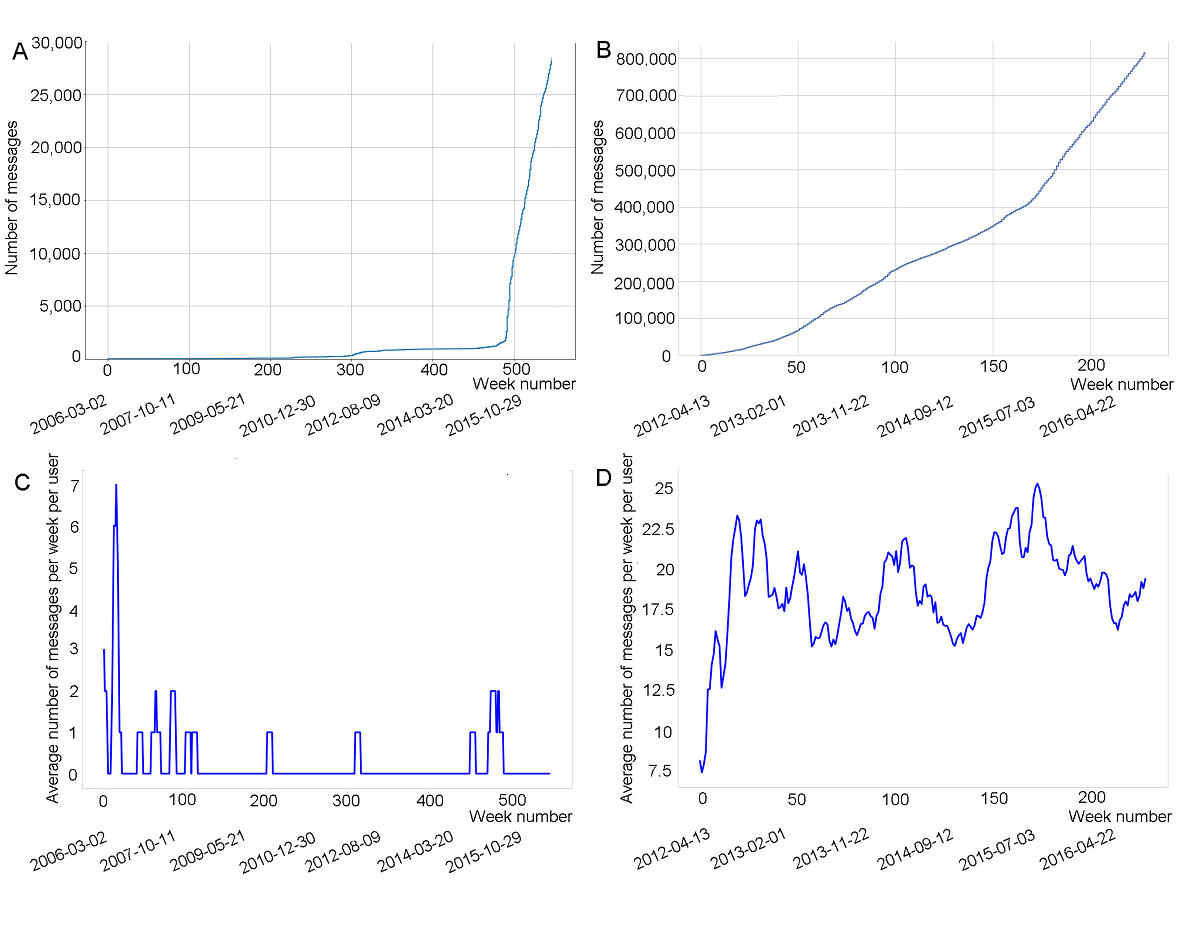
\includegraphics[width=\textwidth ]{Activity.png}
    \caption{Cumulative distributions of the number of posts as a function of time (weeks) within the Asthma UK (A) and the British Lung Foundation (B) communities. Calendars dates are reported below as week numbers (since the inception of the community). Panels C and D illustrate the average number of posts per user per week within Asthma UK and British Lung Foundation, respectively}        \label{fig:activity}
\end{figure}
To calculate the activity patterns of users on these forum, we first work with the most basic of proxies, which is the weekly/daily activity. We arrive at it by calculating the amount of messages exchanged in a community across the whole life cycle of the data. This metric would expose how much activity is happening on a daily or weekly basis on a particular community. It is worth noting that this activity pattern would also shed light on how users are engaging with the community. A continuous engagement is good for the vitality of a community, however if a community revolves around purely functional interactions, you may see a bursty nature of user activity across time~\cite{panzarasa2015emergence}. 

Figure ~\ref{fig:activity} shows the activity patterns on both the health communities on a cumulative and weekly basis. It was quite evident that the BLF community was more active of the two, in that, the community exhibits a consistent engagement by the users across the lifetime of the data as well as on a weekly basis. The Asthma forum however shows a bursty nature, despite being more than twice as old as the BLF community. One possible explanation can arise from the nature of these two illnesses. Asthma tends to be an episodic disease, with flare-ups in patients happening from time to time. These flare-ups are also often seasonal in nature, happening in sync with the pollen cycles in the air~\cite{dellavalle2012effects}. On the contrary, the British Lung Foundation forum deals with, alongside Asthma, diseases that are chronic in nature such as Chronic Obstructive Pulmonary Disorder (COPD) and Emphysema. This means these patients are constantly activated and tend to engage with the community on a more frequent basis. 

\subsection{Cohesive conversations}

\begin{figure}[!ht]
    \centering
    % \hspace*{-5mm}
    \subfloat[]{
        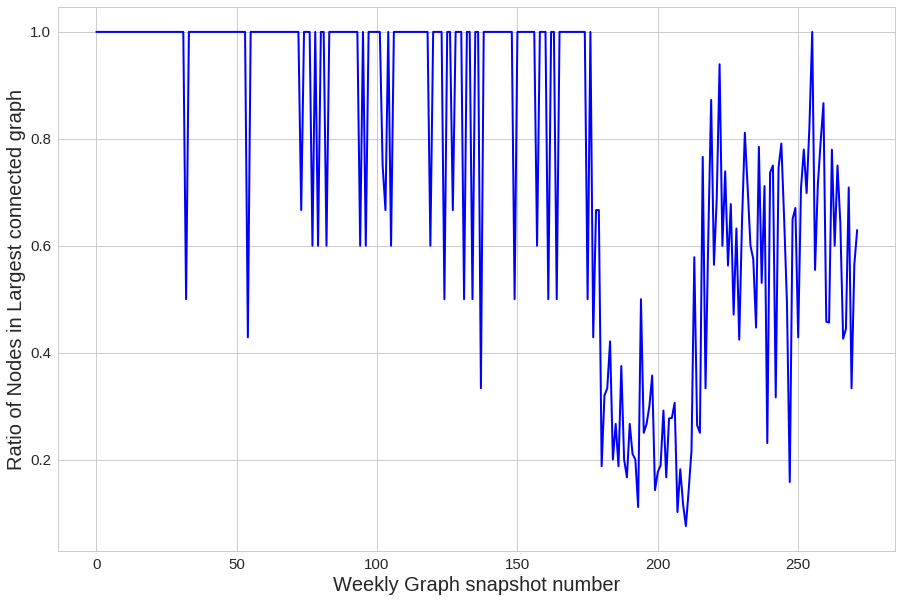
\includegraphics[width=0.5\textwidth ]{ConnectedComponent_weekly_ashtma.png}
        \label{fig:lcc_asthma}
    }
    \subfloat[]{
        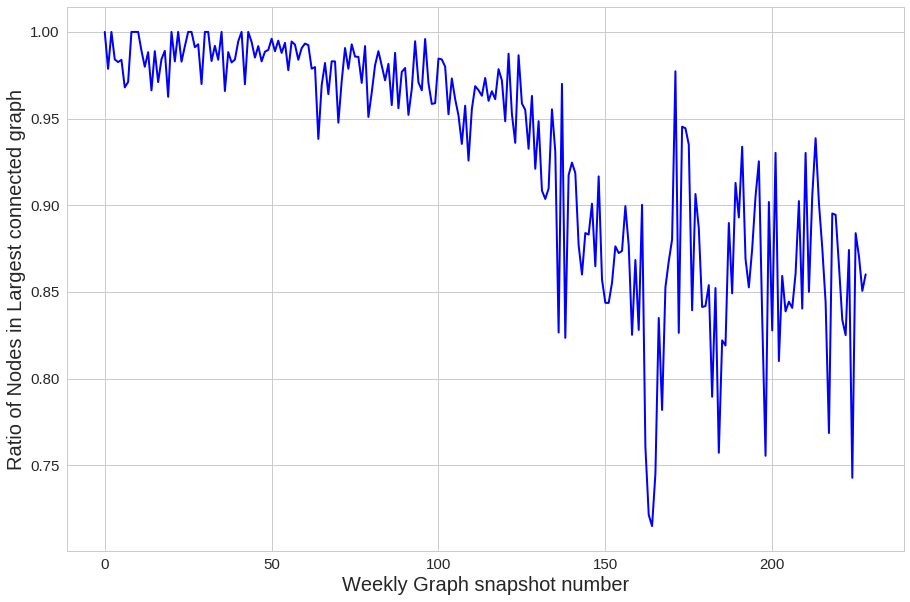
\includegraphics[width=0.5\linewidth ]{weekly_largest_component_BLF.png}
        \label{fig:lcc_blf}
    }
    
    \caption{Fraction of users that are part of the largest component as a function of time (weeks) for Asthma UK \ref{fig:lcc_asthma} and the British Lung Foundation \ref{fig:lcc_blf}.}
\end{figure}

To understand the first aspect of the community's resilience, I examine how is the coverage of communications between the users, on a weekly basis, given that messages are exchanged between the most active users within that week. 
To do so, imagine a sorted list of message interactions over a particular time period $T_k$, sorted in chronological order defined as $L_k=[E_{ij} \forall i,j \in N]$ , where $E_{ij}$ is a message between user $i$ and user $j$, with $N$ total users being active in a given time period $T_k$. Now imagine this time period $T_k$ is of 7 days . I calculate such $K$ lists for the $K$ weeks the community has been active. For each such list, I induce a graph $G_k(V,E)$ such that the nodes in $V$ are the active users in that particular list, and the edges in $E$ are corresponding to the messages exchanged in the list $L_k$ between any two users. 
Now for each such graph $G_k$ I calculate the largest connected subgraph $G_{\theta_k}(N_k,E_k)$ such that all nodes in $N_k$ have at least one path between them. Calculating the fraction $\frac{N_k}{N}$ would give us the total fraction of users who are part of the same conversation network for a given week. After calculating and plotting these fractions across a total of 250 weeks for each community, we see that whenever there is an activity on these networks, almost always, the active nodes belong to the largest connected sub graph. This implies that activity on support forums is cohesive and even if bursty at times, is all encompassing with the users. 

It is worth noting that as the activity on the communities increases, you see an increase in fragmentation of the graph structure with the ration of nodes in the Largest component dropping considerably(See figure \ref{fig:lcc_asthma} and \ref{fig:lcc_blf}). Which means there are concurrent discussions  happening with disjoint set of users. 



\subsection{Fragile global structure}
\label{sec:fragility}
\begin{figure}[!ht]
    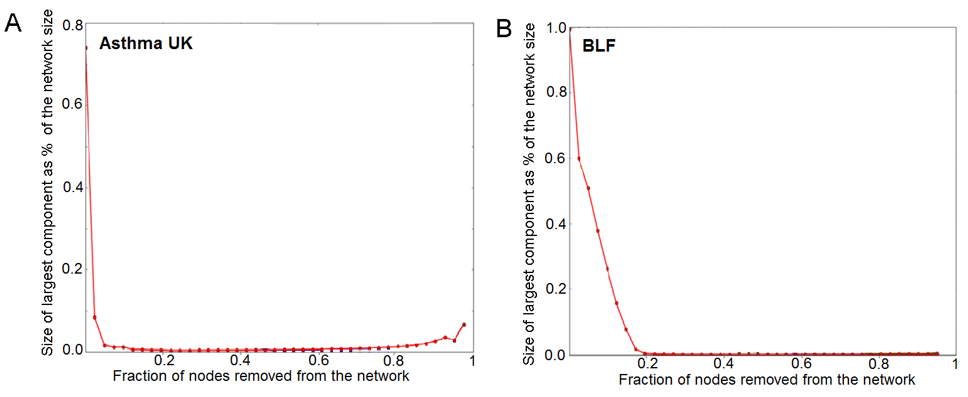
\includegraphics[width=\textwidth]{jmirSensitivity.png}
    \caption{Results of progressive removal of superusers. Both communities collapse drastically, in terms of connectivity, with BLF showing a marginally more resilience }
    \label{fig:sense_asthma}
\end{figure}
Despite the exchange on a weekly basis is quite cohesive, it is pertinent to understand the resilience in terms of user responsibility in helping, in order to examine the health of such a community. Moreover, I want to know if the conversation network is held together by a more or less uniform contribution of nodes, or if there is a skew in the responsibility of nodes. 
This can be tested by using the sensitivity analysis methods, popular in the network science~\cite{braunstein2016network,albert2000error}, which measures the network's capacity to diffuse information as you remove nodes based on certain property. In our case, we want to understand the importance of the \textsl{Superusers}, or the users who are disproportionately more active. Hence we begin by first sorting all the nodes in the macroscopic graph $G(V,E)$ in order of their degrees. The degree of a node in the global graph is proportional to the diverse set of users that node has communicated with, over the period if the community's lifetime. We then start removing nodes from the top, by progressively removing nodes in increments of 1\%. I then compute the size of the largest connected component $G_k$ and compute the ration of number of nodes in $G_k$ as compared to the original global undisturbed network.  Figure \ref{fig:sense_asthma} shows the performance of global graphs of both the communities to this attack. It is worth noting, that what we observe is that a top 10\% nodes by activity are responsible for most of the cohesive connectivity of the community. This also means that the top 10\% of these nodes have the most diverse connections in terms of number of users contacted. This gives hope to health care industry, since these nodes can act like efficient information diffusers, if used in a targeted fashion. 

\subsection{Anti-rich conversations}
\label{sec:richclub}
\begin{figure}[!ht]
    \centering
    % \hspace*{-5mm}
    \subfloat[]{
        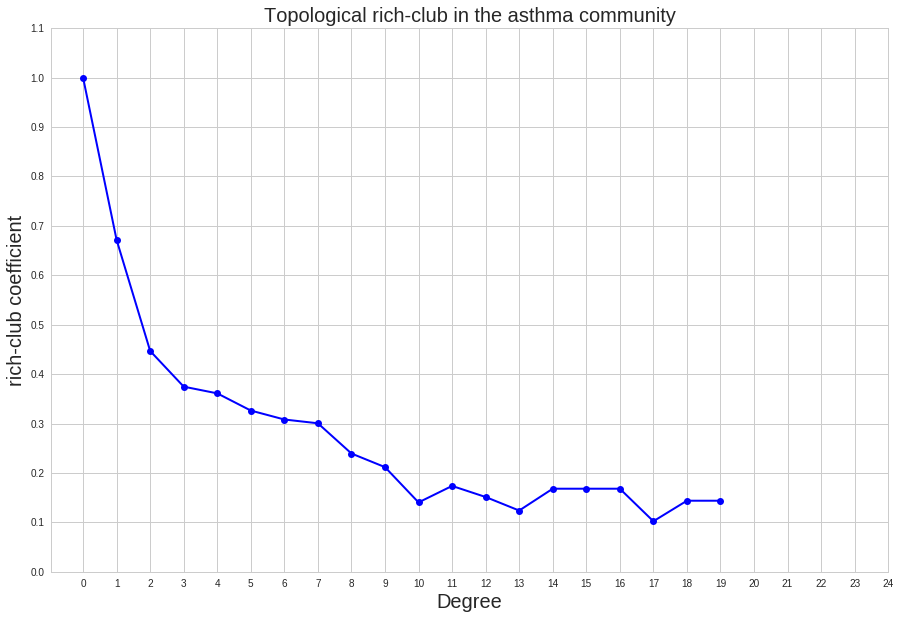
\includegraphics[width=0.5\textwidth ]{RichClub_asthma_truncated.png}
        \label{fig:rich_asthma}
    }
    \subfloat[]{
        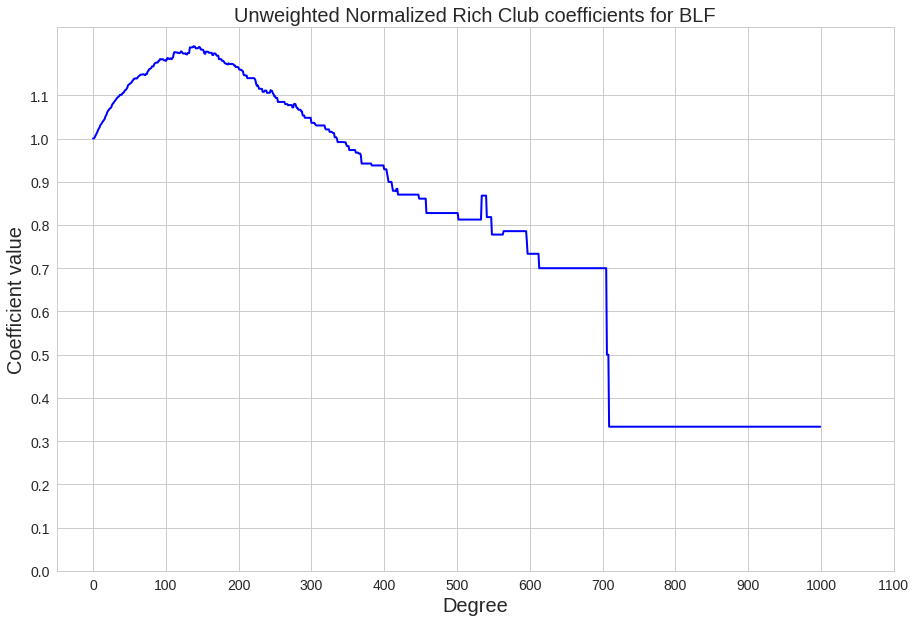
\includegraphics[width=0.5\linewidth ]{RichClub_BLF_truncated.png}
        \label{fig:rich_blf}
    }
    \caption{ Plots of rich-club coefficients for each viable degree in the respective communities. Both communities exhibit values less than 1, indicating an anti-rich behaviour by the well connected nodes.  }
\end{figure}
The “rich-club” coefficient is a metric designed to measure the extent to which well-connected users tend to connect with one another, to a higher degree than expected by chance~\cite{colizza2006detecting}. To this end, for each value k of a node’s degree (ie, the number of other users a given user is connected with), we computed the ratio between the number of actual connections between nodes with degree k or larger and the total possible number of such connections~\cite{opsahl2008prominence}. We then divided this ratio by the one obtained on a corresponding random network with the same number of nodes and degree distribution (ie, the probability distribution of the degrees over the whole network) as the real network, but in which links were randomly reshuffled between nodes. 

Formally let $G(V,E)$ be a global graph representation of the community. Let $V_{>k}$ be the set of vertices in the graph having degree higher than $k$. Let there be $N_{>k}$ such vertices having $E_{>k}$ edges between them. In such case, the rich club coefficient for degree $k$ in the graph $G$ is given by 
\begin{equation}
 \phi(k) = \frac{2E_{>k}}{N_{>k}(N_{>k} - 1)}
 \label{eq:rich_club}
\end{equation}
In this equation $\frac{N_{>k}(N_{>k} - 1)}{2}$ represents the maximum number of edges possible between $N_{>k}$ nodes. These coefficients are highly dependent on the size of the network, which makes them hard to compare. So I normalize the network by comparing against a random null model of rich-club coefficients $\phi_{rand}(k)$. This is obtained by generating an ensemble of random networks, each having the same degree distribution as that of $G$, but with links randomly placed. The ratio $\frac{\phi(k)}{\phi_{rand}(k)}$, gives us an un-correlated trend about the rich-club effect in $G$. 

Thus, the rich-club coefficients may take values lower or higher than 1, depending on whether the real network has a higher or lower tendency to coalesce into rich clubs than randomly expected. In particular, networks that display a high rich-club coefficient (ie, greater than 1, are also said to show a “rich-club effect,” namely the tendency to organise into a hierarchical structure in which highly connected nodes preferentially create tightly knit groups with one another ~\cite{mcauley2007rich}. .

In most previous studies the rich-club coefficient in the technical and real world networks exhibits values larger than 1 as the degree of a node goes up. This shows a propensity to create rich-clubs, with highly connected nodes preferentially connecting with other highly connected nodes. Thus these networks exhibit exclusive clubs of (topologically) rich nodes, as illustrated in previous work~\cite{zhou2004rich,colizza2006detecting}. What we observe however in the cases of support communities is that in general we end up with a less than 1 rich-club co-efficient as the value of degrees $k$ goes up. This means, rich nodes are exhibiting an anti-rich behaviour, where nodes which have a higher degree prefer in engaging with new nodes with lower degree. This implies an active information exchange from a well connected node to a sparsely connected node, which we would expect in a supportive interaction according to the definition of social support.


\section{What differentiates \textbf{users} on support communities from generic ones?}
\label{sec:support}
Once we establish that these support communities are thriving and are providing what seems to be an active supportive environment for the users(anti-rich superusers), it is worth delving into the analytical methods for quantifying these supportive interactions. More so we would like to have concrete metrics that characterize a given community as a supportive one. To do so we need to understand how are the users on these communities driven to help each other, and whether there is a correlation between the ``richness'' of a user, as defined in previous section, and its propensity to help. More so we would like to know how consistent are these so called ``rich'' users in providing support. 

\subsection{Propensity to help} 
We would like to understand how users on support communities, as a group behave as they become more seasoned. Fortunately, there is an approximate way for us to capture a user's role as a support seeker and as a support giver. As described in Section \ref{sec:dataset}, the forum activity consists of a root poster, asking a question to the forum board, and the members responding to that question in a cascaded fashion. These responses, along with the original question constitute what is called as a \textsl{thread}.
To that end, we define the following two roles on these communities\footnote{There are other ways to qualify someone as support giver/seeker, mainly using language sturcture, but here we consider only the bare minimum requirement to be considered as one, using the position in conversation structure}

In the context for support forums, a support seeker is a user who begins a thread by posting on the forum, a question, or a query, to which others may respond to. Similarly a support giver is a user who responds to any post by a support seeker.

With this in mind, I aim to model the behaviour if users on these support communities in terms of being a support giver or a support seeker.

We first begin by calculating the average number of questions per user and answers per user across the dataset, by finding the mean number of questions and answers posted by any user on the forum. 
We consider an expected probability of answering a question by a user as $P_a$ as 2/3 and the probability of posting a question as $P_q$ as 1/3. 
With this information we modify the definition of ``Z-score'' to quantify the expertise, used by Adamic. et. al ~\cite{zhang2007expertise} to arrive at the expression of expertise in the context out our support community. 

 A user has two possible actions at any given time, while interacting with the community. They can either post a question on the forum, or answer to existing questions. The probability of doing either actions are $P_a$ and $P_q$ respectively. To that end, we try to model this interaction process as a Bernoulli process with two outcomes, having asymmetric probabilities. 
 
\begin{proof}
   
    Consider a Bernoulli process for a user to choose to answer or post a question on the forum, with asymmetric probabilities for answering ($P_a$) and posting a question ($P_q$). 
    For any user $i$ the total number of posts $n_i$ are the sum of total number of questions posted $q_i$ and answers posted $a_i$ and $n_i = a_i + q_i$
    For a Bernoulli process the variance for the whole forum is given as: 
     $$\sigma_{forum} = \sqrt{nP_a(1-P_a)}$$     $$\sigma_{forum} = \frac{\sqrt{2n}}{3}$$
    Similarly the mean for this process can be written as : 
    $$ \mu_{forum} = nP_a = \frac{2n}{3} $$
    $Z_{score}$ of a random variable $X$ is defined as 
    $$Z_{score} = \frac{X - \mu}{\sigma}$$
    Substituting the values for $\sigma_{forum}$ and  $\mu_{forum}$ inside the expression for $Z_{score}$ we arrive at the modified Z-score as 
    \begin{equation}
        Z_{score} = \frac{a-2q}{\sqrt{2(a+q)}}
    \label{eq:zscore}
    \end{equation}    
\end{proof}
Equation \ref{eq:zscore} depicts the modified notion of Z-score for the question answering process of our support community. I calculate this particular metric for each user in both the communities based on their posting history. 
\begin{figure}[!ht]
    \centering
    % \hspace*{-5mm}
    \subfloat[]{
        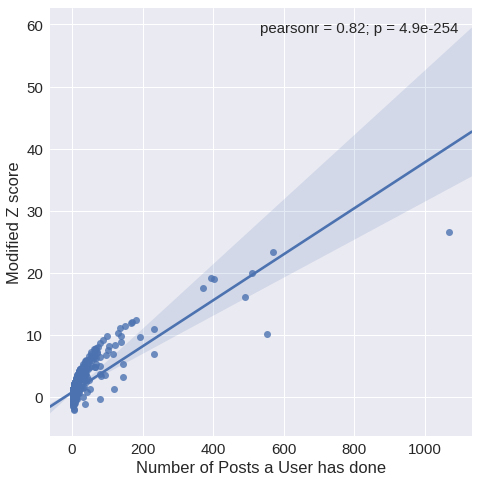
\includegraphics[width=0.5\textwidth ]{ModifiedZScore_asthma.png}
        \label{fig:zscore_asthma}
    }
    \subfloat[]{
        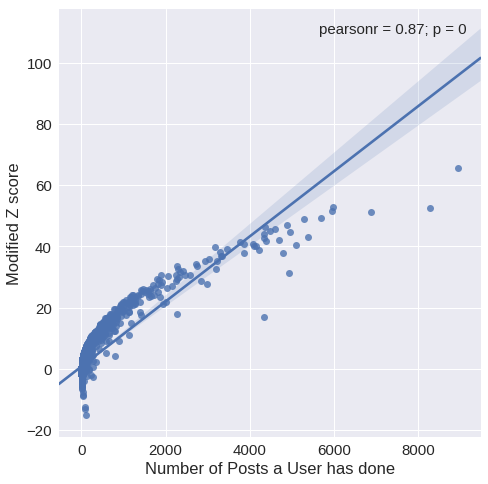
\includegraphics[width=0.5\linewidth ]{Modified_ZScore.png}
        \label{fig:zscore_blf}
    }
    \caption{ Scatter plots for the $Z_{score}$ values for (a) Asthma UK community and (b) British Lung Foundation community. Both communities show a strong positive correlation between a user's activity and their propensity to answer questions. }
\end{figure}

I then find the correlation between a users Z-score and the total number of posts a user has done in their lifetime on the forum. Figure \ref{fig:zscore_asthma} and Figure \ref{fig:zscore_blf} shows the results of this analysis for both the communities. It is quite evident, that as the users become more seasoned and post more actively, they are more likely to answer on questions rather than post new ones. This also implies that based on the rich club results from Section \ref{sec:richclub}, these communities are thriving not only for the ``rich'' users, but also for the sparse users. Users on these communities are more open to new members and provide active support to them. 
Developing metrics like this makes quantifying whether a particular community works for the subscribers a tractable problem.


\subsection{ Superusers and structural holes }
One of the key aspects of utility of any social network is driven from the social capital offered as a result of the subscription. 


Till now we looked at the global macro structural properties of this support graph using the global graphs $G_g$, where we look at the user's interactions with other users across the lifetime of the community. But often the supportive interactions happen in a lifetime of a single thread, revolving around a topic or query. So to examine the effect of the superusers on the social cohesion, we correlate the total number of posts done by super users on any given thread, to the amount of closed triangles found in the corresponding thread graph $G_t$.  

\begin{figure*}[!ht]
    \centering
    % \hspace*{-5mm}
    \subfloat[]{
        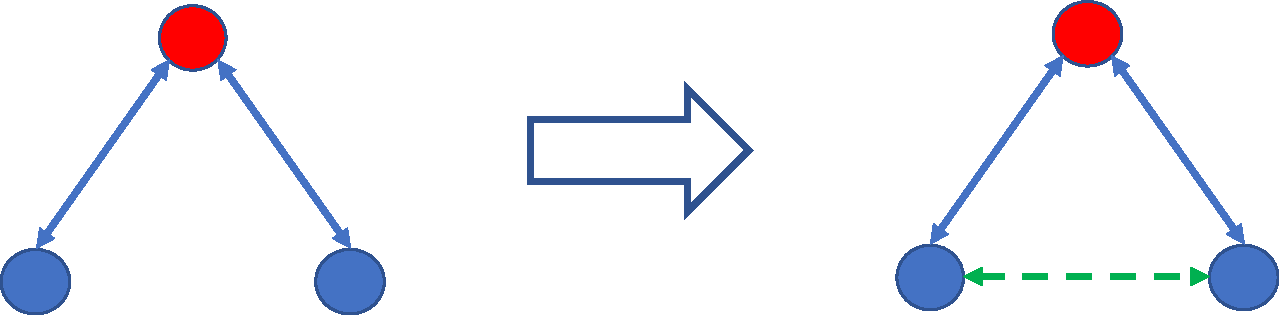
\includegraphics[width=\linewidth]{Closure.pdf}
        \label{fig:closure}
    }

    \subfloat[]{
        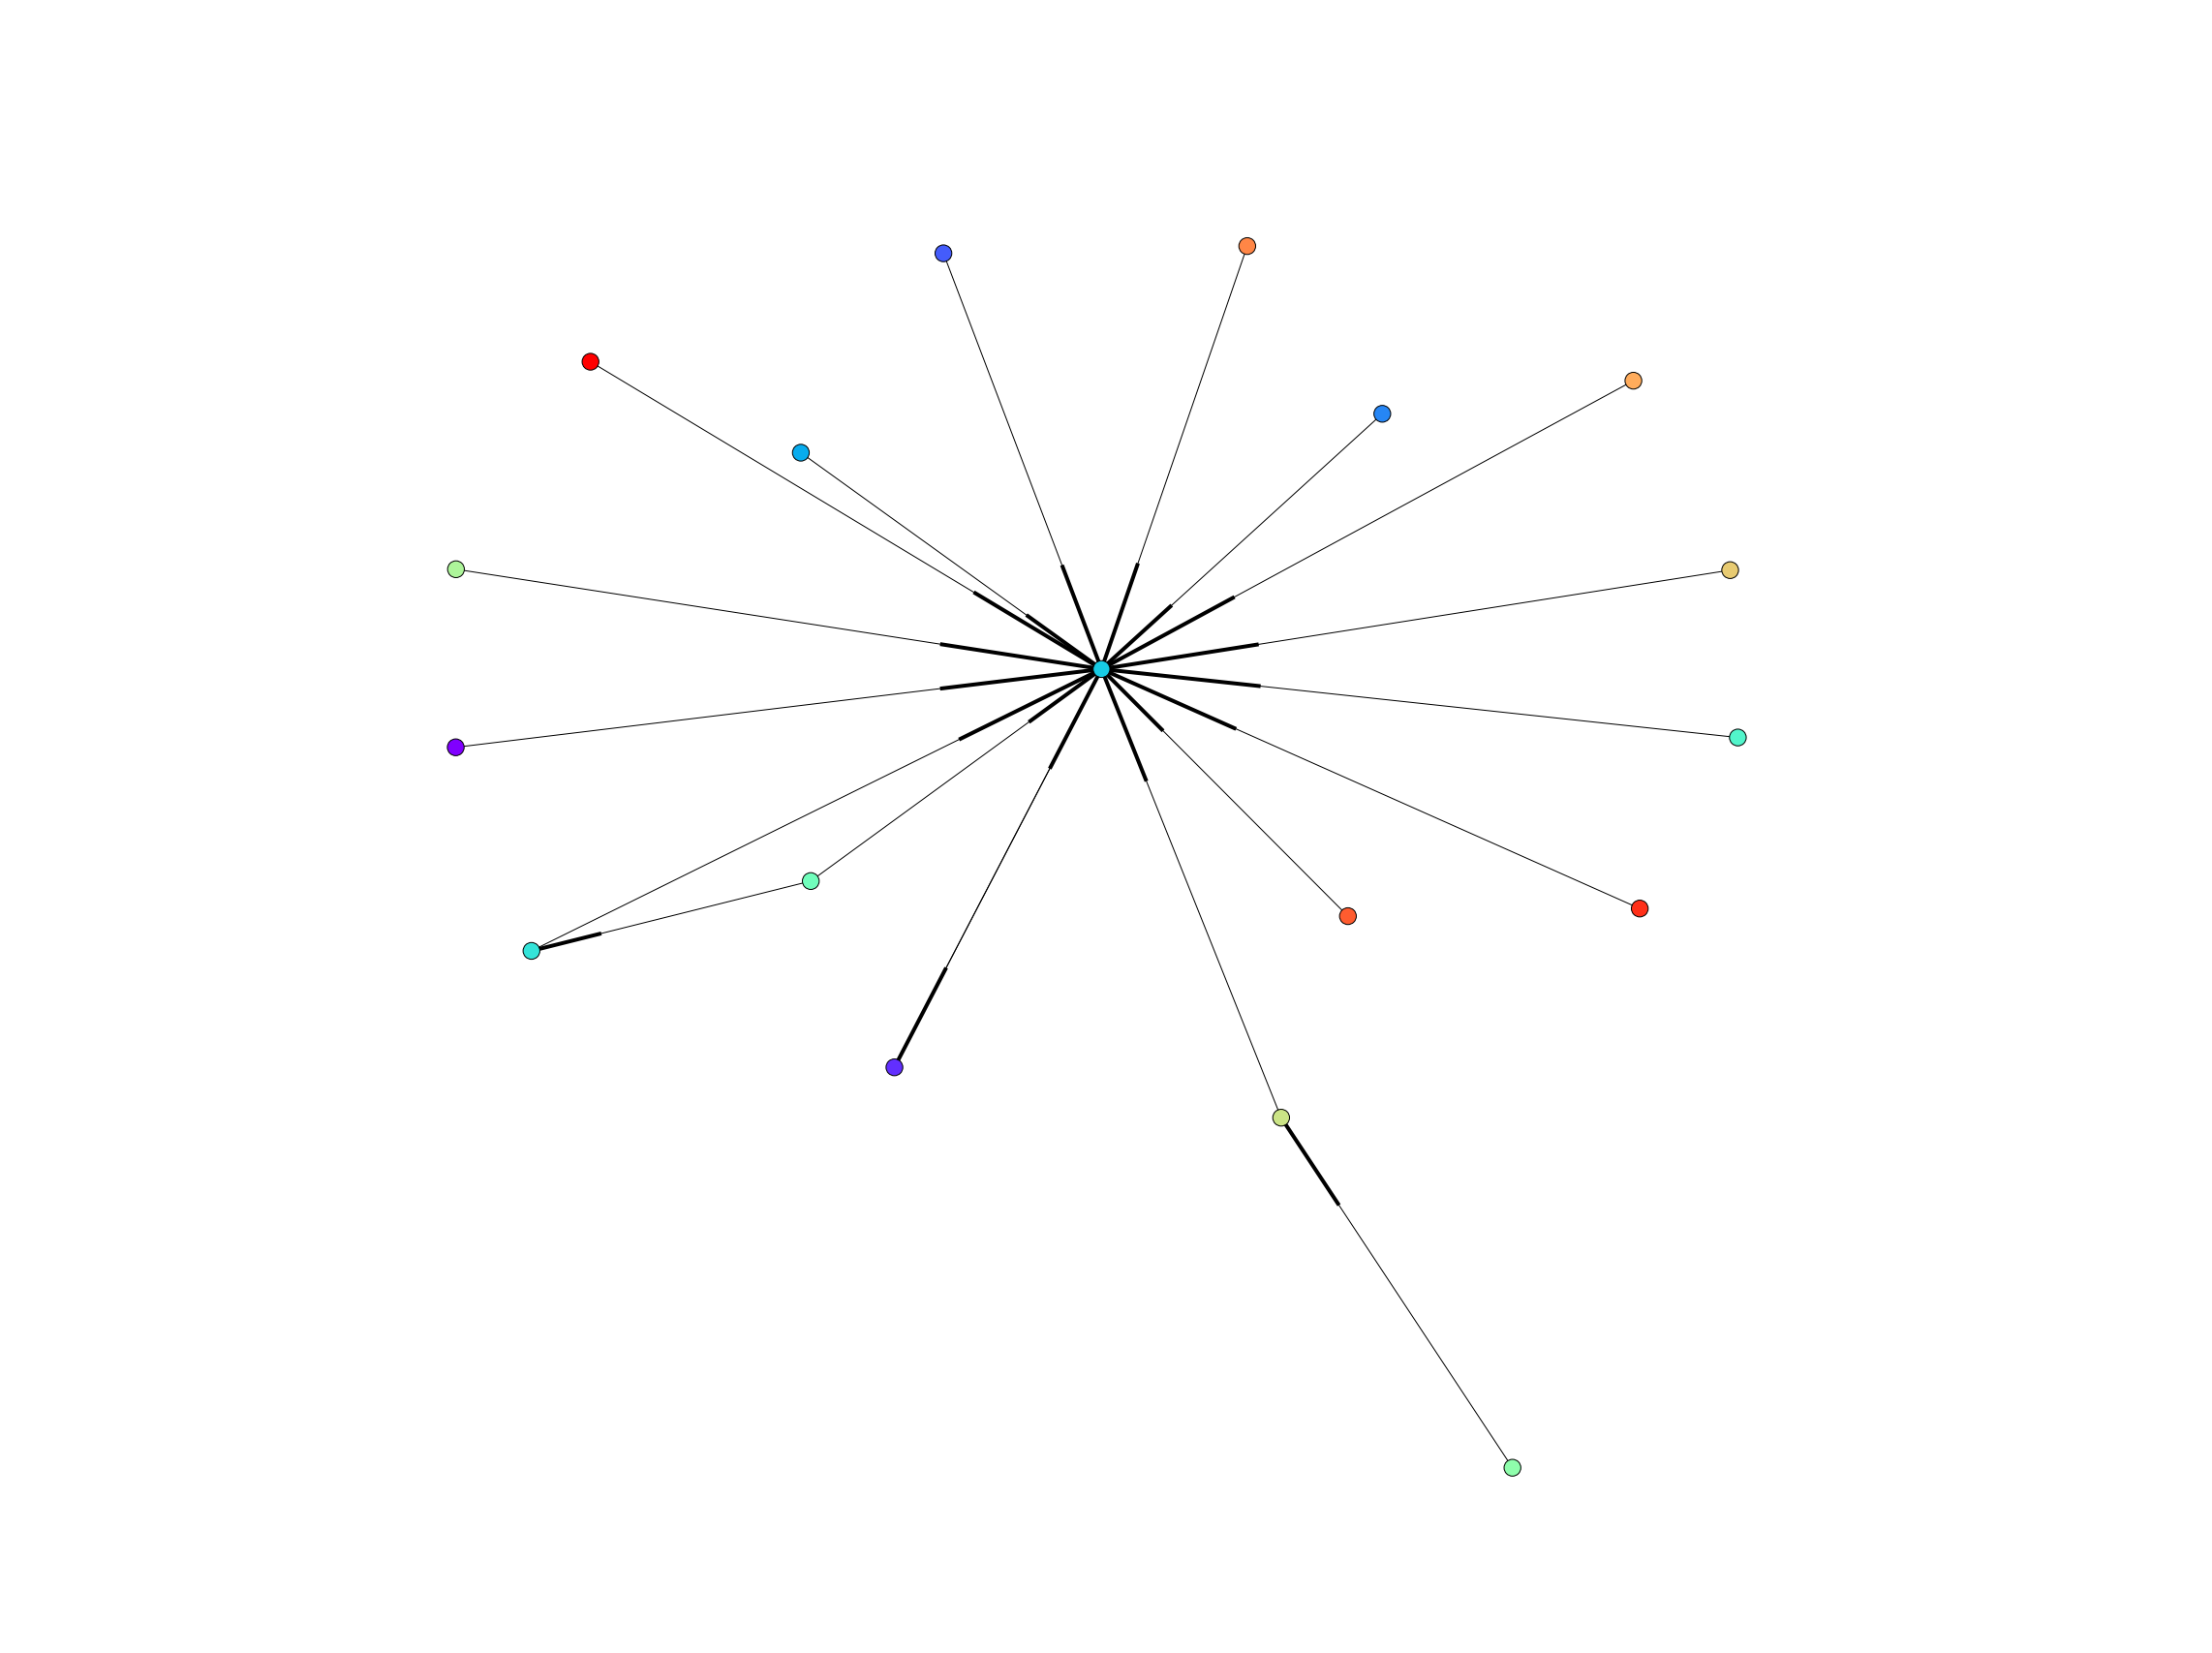
\includegraphics[width=0.5\linewidth ]{LowOPActivityGraph.png}
        \label{fig:noTri_op}
    }
    \subfloat[]{
    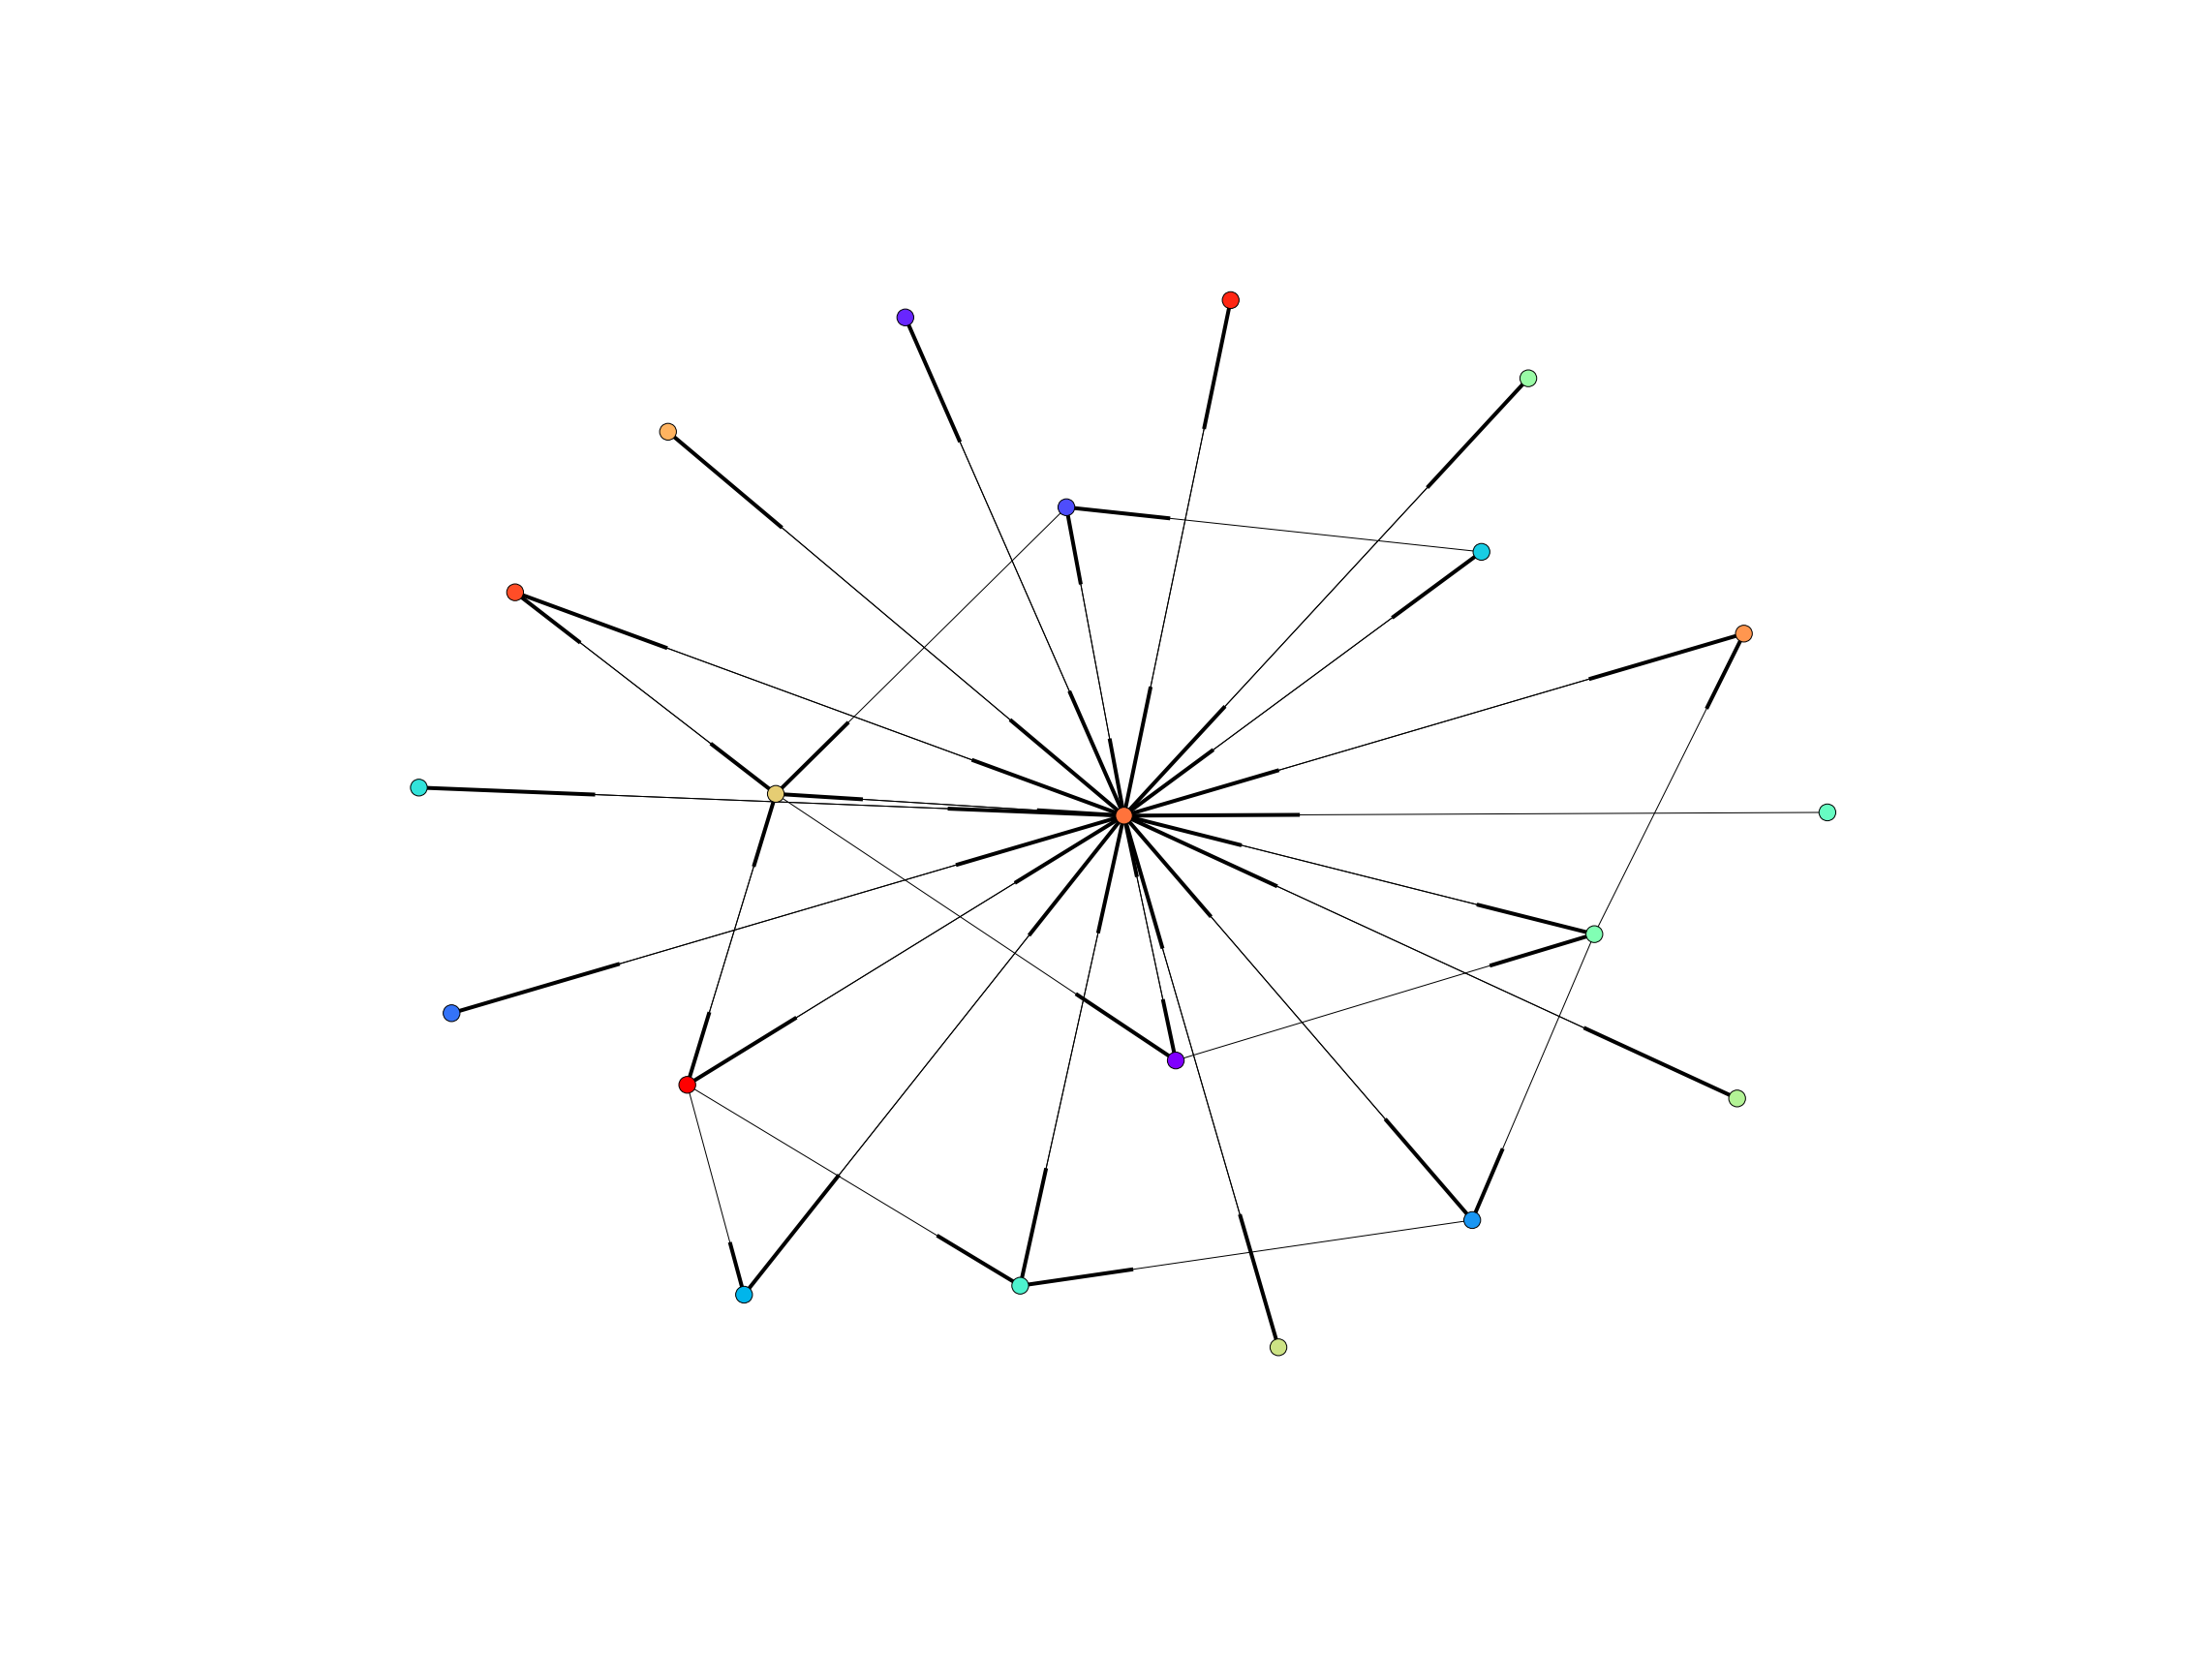
\includegraphics[width=0.5\linewidth ]{HighOPActivityGraph.png}
    \label{fig:Tri_op}
    }
    \caption{ Figure~\ref{fig:closure} shows an example of closure among three nodes, where a structural hole between a cluster of three nodes is closed by addition of the green link. Figure~\ref{fig:noTri_op} shows a thread level interaction graph showing lots of structural holes between participating nodes. On the other hand Figure~\ref{fig:Tri_op} shows an example of a thread level interaction graph where a `rich' user has contributed multiple times. This graph also shows more closures }
\end{figure*}

The resultant scatter plot can be seen in Figure~\ref{fig:TriCorr}, where we can see a net positive correlation of 0.44, with a very low p-value. This means there is a general trend of higher triadic closures in a conversation, with the amount of rich user participation.
 
\begin{figure}[!ht]
\centering
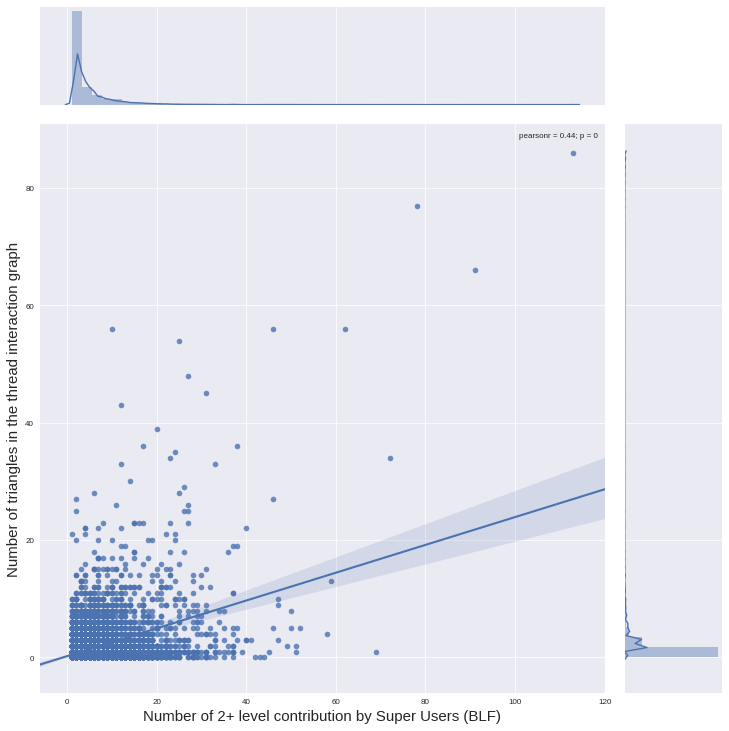
\includegraphics[width=0.7\linewidth ]{SUParticipationTriangles.png}

\caption{Scatter plot between the number of closed triangles in a conversation thread, with the total number of posts done by a superuser in that thread. A positive correlation of 0.44, with a p-value of 0 is observed. This indicates that the presence of a super user in a thread improves the over all cohesion of that thread and closes structural holes}
\label{fig:TriCorr}
\end{figure}

\section{Discussion}
In this chapter, we found that support communities show peculiar temporal and interaction dynamics. \textbf{RQ1} asked about the dynamics of support communities. We find that support communities exhibit a high level of engagement and participation. The communities are held together by the superusers. The removal of these superusers, collapses the network structure of these communities. \textbf{RQ2} asked about differentiating properties of users on support communities. We find that the users exhibit an anti-rich behaviour. This means that the superusers are engaging with less active users and are practising inclusion. We also find that users on support communities progress onto being support givers from support seekers with time. 
The idea of perceived support stems from the fact that the user in distress is not only getting the crucial information about the disease, but also benefits from the social capital of the allied users. We observe that  superusers tend to have a positive effect on the social capital of a conversation, promoting more social cohesion.

There is immense value in understanding how social support thrives on the internet, especially because of its potential to relieve the load off the ever so burdened health services. 
The work till now focussed on the global interactions of support givers and seekers on a community. It investigated the dynamics of support communities and looked at individual user's role in the larger scheme of things. 

In the next chapter we would explore the role of the conversation structure from the scale of an entire conversation(macro) and from the scale of the immediate local interactions in the ego network of a user(meso). This goes beyond looking at the individual actors of support, and quantifies the peculiar structure of a supportive conversation on the web.
%*******************************************************************************
%****************************** Second Chapter *********************************
%*******************************************************************************

\chapter{Online health social networks}

Online communities have the potential to influence health and health care. Recent studies have suggested that the participation of people with long-term conditions (LTCs) in online communities (1) improves illness self-management [1], (2) produces positive health-related outcomes [2-4], (3) facilitates shared decision-making with health care professionals [5,6], and (4) may even reduce mortality [7].

There is also evidence that self-management support interventions can reduce health service utilization [8,9].

Online communities have experienced an upsurge in popularity among people with chronic respiratory conditions such as cystic fibrosis [10], asthma [11], pulmonary hypertension [12] and chronic obstructive pulmonary disease (COPD) [13]. More than 15 million people in England suffer from a long-term condition or disability, and they account for at least 50 percent of all general practitioner appointments [14,15]. Thus, assessing how these online communities function and evolve can have important implications for health care provision.

This form of “user-led self-management” of LTCs bears similarities with the “expert patient” model, an approach to self-management of LTCs produced by the United Kingdom (UK) Department of Health in 2001 [16]. Evidence of the effectiveness of conventional off-line self-management programs based on the expert patient model, though, has been weak [17]. Clinic-based self-management programs often failed because of: (1) lack of awareness and engagement among patients and staff, (2) failure to consider low health literacy or cultural norms, (3) lack of attention to the need for family and social support, and (4) a fragmented approach to the provision of health and social care [18]. Although online health communities can be seen as an extension of the expert patient model, network effects, in addition to the online disinhibition effect [19], make them a distinct and unique complex intervention mechanism.

On average, one in four people with an LTC who use the Internet tries to engage online with others with similar health-related concerns [20]. In particular, it has been suggested that the value of participating in an online community lies in the possibility of gaining access to a range of people and resources quickly, easily [21], and anonymously [4], as well as obtaining tailored information and emotional support [1,22-26]. However, most of this evidence comes from qualitative studies [1,27], whereas only recent years have witnessed an increasing interest in quantitative assessments of online communities as intervention mechanisms [28-33]. Recent studies have been concerned with the users’ unequal contributions and engagement patterns, and with the role of superusers. However, the contribution of superusers to the sustainability of online health communities and their structural properties remains mostly unclear.

The potential future integration of online health support systems with formal health care provision should be underpinned by a better understanding of how they are used and by evidence of their effectiveness. Indeed, as suggested by the Medical Research Council [34], integrating online support systems with the more traditional health care provision would require the identification and comparative assessment of potential alternative intervention mechanisms.

An expanding body of literature concerned with social network analysis has examined the structural patterns of relations among interacting actors and the social mechanisms that enable them to gain access to valuable resources [35]. There is also increasing evidence that network approaches can be applied to understanding the users’ “expertise” [36], their interactions, and network effects on health-related outcomes in online health communities [37,38]. Uncovering the mechanisms underlying the formation of successful social networks requires a study of how online connections among people, namely the social ties or links, emerge and evolve, and how groups of individuals gradually grow in membership and become interconnected with one another. These processes of tie creation and group formation in online patients’ communities are still mostly unexplored [1].

In this study, we performed a network analysis of the structure and dynamics of two online communities of people with LTCs. We chose the Asthma UK and the British Lung Foundation (BLF) communities as an exemplar of such communities because their users typically suffer from chronic respiratory conditions. In particular, while Asthma UK users typically suffer from a respiratory condition characterized by variable and recurring symptoms, BLF users represent a more heterogeneous population of participants affected by different diseases linked to chronic symptoms of breathlessness (eg, COPD, pulmonary fibrosis, cystic fibrosis, and lung cancer).
We aimed to uncover and understand how these communities function and evolve, and the role that some users have in maintaining integration and cohesion (see Textbox 1 for research questions). Ultimately, this study provides evidence for gauging the effectiveness of different interaction patterns and the users’ structural positions and their potential for enhancing and sustaining health online communities as scalable self-management support interventions.\textbf{}




\section{Dataset and properties}
Data were collected by HealthUnlocked [39], the online platform provider of the Asthma UK and BLF communities. Registered users can choose to either write posts publicly or send private posts to one another. In the latter case, posts are shared between 2 users only, whereas when posts are written publicly, a large number of users can become connected through threads of posts. Only posts that were shared publicly were collected and analyzed. For this study, user identifiers (IDs) were anonymized by HealthUnlocked, and no demographic information was collected. The data sets included posts and their metadata (ie, the anonymized user ID numbers), user roles (eg, user, administrator, or moderator), date of posting, the hierarchical level of the post within the corresponding thread, and the dates in which the users joined and left the community. Both communities were moderated, and HealthUnlocked moderators (identified through metadata linked to posts) were included in the analysis to assess their contribution and compare it with other users. Online communities on the HealthUnlocked platform benefit from additional functionalities compared to other online forums, such as built-in patient groups that moderate the content. In particular, the content accessed by users is tailored to their interests, and profiles highlight users’ condition, chosen community, medications and treatments they use or find interesting. No data were collected on participants’ characteristics, though only people declaring themselves to be older than 16 years were permitted to create an account and take part in the online communities.


\section{Graphs: A primer}



\section{Activity patterns of users}

We looked at the number of users, the number of posts and connections per user and posting frequency. A connection (ie, a tie, link, or edge) was established from one user to another when the former replied to a post by the latter (see Textbox 2 for network analysis terminology). The pattern of connections generated over time through the cumulative number of posts and replies was examined. We were interested not just in the number of posts and responses but in who responded to whom, and when. To this end, we used social network analysis [40] to visualize and study the structure of the relationships between users. Both visualization and analysis were conducted using the Gephi software. The network analysis was carried out through additional custom computer code in python. Descriptive analysis of the networks (ie, number of users, posts, and posting frequency) were calculated using the Pandas library, an open source library providing data structures and analysis tools for the Python programming language.

As a result of the small percentage of users who wrote posts to a disproportionally high number of users, the users’ activity showed long-tailed distributions. Therefore, our analysis was based not only on means and standard deviations but also on medians.

To uncover time patterns in posting activity, we used Fourier transforms of the time series of the users’ activity [46], a known method used for the analysis of signals. Through Fourier transforms, we identified the frequency components, called harmonics, that together made up the posting activity stream. In other words, we regarded the posting activity over the entire observation period in both communities as a complex signal and identified the frequency components that made up such a signal. This analysis was performed using custom code in Scipy, a Python-based scientific computing library.

The “rich-club” coefficient is a metric designed to measure the extent to which well-connected users tend to connect with one another to a higher degree than expected by chance [43]. To this end, for each value k of a node’s degree (ie, the number of other users a given user is connected with), we computed the ratio between the number of actual connections between nodes with degree k or larger and the total possible number of such connections [47]. We then divided this ratio by the one obtained on a corresponding random network with the same number of nodes and degree distribution (ie, the probability distribution of the degrees over the whole network) as the real network, but in which links were randomly reshuffled between nodes. Thus, the rich-club coefficients may take values lower or higher than 1, depending on whether the real network has a higher or lower tendency to coalesce into rich clubs than randomly expected. In particular, networks that display a high rich-club coefficient (ie, greater than 1) are also said to show a “rich-club effect,” namely the tendency to organise into a hierarchical structure in which highly connected nodes preferentially create tightly knit groups with one another, thus generating exclusive clubs of (topologically) rich nodes, as illustrated in previous work [48].

In our study, superusers were defined according to their cumulative activity over the entire observation period. In total, we identified 400 superusers. To uncover how many superusers were active within each week, we detected how many unique users, among the 400 identified over the entire period, were active within that time window.

Following Zhang et al [36], the “z-score” was used as a proxy for users’ expertise. According to this measure, replying to many questions suggests one’s expertise, while asking questions indicates lack of expertise. In our analysis, we treated anyone starting a thread as a help-seeker, and anyone commenting on the thread as a help-giver [36]. Accordingly, the proposed z-score aims to capture the combined help-seeking and help-giving patterns. To this end, for each user, we measured how many standard deviations the observed total number of the user’s help-giving posts lies above or below the expected number of help-giving posts for the whole system. We extended the approach proposed by Zhang et al by empirically assessing the probability of posting and answering a question across all users over the entire observation period. In the BLF community, we found that the probability of answering is Pa=2/3, while the probability of posting is Pq=1/3. We assumed a Bernoulli process of posting an answer or a question to the forum, with probabilities defined as above. The z-score for a given user i was calculated according to equation (a) in Figure 1, where ai refers to the total number of answers user i posted to the forum, qi is the total number of questions user i asked in the forum, and ni=ai +qi is the total number of messages posted by user i.
To obtain $Zscore_i$, let us define a random user that posts the same total number of messages nrandom to the forum as user i (ie, nrandom=ni). We would expect this random user to post an average number of answers to the forum given by equation (b). Plugging in the value of $Pa=2/3$, we obtained equation (c). Similarly, we would expect the random user to post answers with a standard deviation given by equation (d). Plugging in the value of $Pa=2/3$, we obtained equation (e). To measure how many standard deviations above or below the expected random value a user i lies, we then computed Zscorei according to equation (f). Plugging in the values of $\mu_{random}$ and $\sigma_{random}$, we obtained equation (g). Finally, by substituting $ni=ai +qi$, we obtained equation (h). 

\section{Dataset charactarization}
The data sets span, respectively, 10 years for the Asthma UK and 4 years for the BLF communities (see Table 1).

Despite the shorter time span, as a result of the larger number of users, the number of posts in the BLF community was higher than in Asthma UK, namely 875,151 compared to 32,780 respectively. Moreover, BLF users wrote a higher number of posts per user and were connected with a higher number of other users when compared with people in the Asthma UK forum (see Figure 2). In both communities, 60\%-70\% of registered users wrote no posts (ie, they were lurkers). Users who wrote more than one post contributed with a median of 8 (range 2-8947) and 5 (range 2-1068) posts in the BLF and Asthma UK communities, respectively.

The number of official moderators among the highly active users was negligible; there were no moderators in the top 5\% contributors to BLF and only 2 in the top 5\% for Asthma UK. Thus, our network analysis predominantly reflects content originated from registered users.

When classified according to posting activity (ie, number of posts written to the forum), the top 5\% users contributed to a substantial proportion of all posts: 58\% and 79\% in the Asthma UK and BLF communities, respectively. Superusers were those who made a high number of connections with other users in both Asthma UK and BLF communities (see nodes of large size in Figure 2). Asthma UK superusers made a lower number of connections than BLF ones. The posting activity of these superusers will be analyzed in more detail in subsequent sections.
\subsection{Activity}
Posting Activity

The cumulative number of messages posted grew uniformly over time in the BLF community. By contrast, in 2015, the Asthma UK forum witnessed a substantial increase in posting activity, at a time coinciding with its move to the HealthUnlocked platform (see Figure 3A and B). This increase in activity can be attributed to the online community functionalities offered by HealthUnlocked, as described in the Methods.

The number of posts per user per week oscillated around a decreasing and an increasing trend (Figure 2C and D), while at the same time the number of posts always went up over the study period (Figure 1A and B). This suggests that there were intervals of time during which the rate of increase in new users was larger than the rate of increase in total posts. Moreover, in the Asthma UK forum users wrote according to two time patterns—they posted at an interval of 1-20 days or 6 months (Figure 4A), while those in the BLF community at an interval of 2 days (Figure 4B).

As more users joined the communities and connected to one another through online posts, distinct groups of connected users started to emerge. These groups, called network components (see Textbox 2), have fundamental implications for the effectiveness of processes of network dynamics such as information diffusion [49]. In a relatively short period, both communities underwent the formation of the “largest component” of connected users, namely a connected subset of users whose size increasingly outgrew the size of all other components (see Figures 1 and 4, and Multimedia Appendices 1 and 2). The largest connected components in both communities included 60%-100% of users.

Figure 5 suggests that, as time went by, the number of forum participants and their posting activity increased, and the proportion of users who were part of the largest components decreased. This finding was expected because the number of posts also rose exponentially, yet at times at a lower rate than the one at which new users joined the communities (see Figure 1C and D). It, therefore, became more difficult for the network to self-organize into a connected component that would include 100\% of the users. Figure 5A also shows that around week 450, when the forum moved to the HealthUnlocked platform, a larger fraction of users began to join the largest connected component, thus highlighting the role that the new online platform played in strengthening the connectedness of the network (see also Figure 3A and B).
\section{Propensity to help} 


\section{Not like conventional networks: Anti-rich club effect}


\section{Key takeaways, possible interventions}


\chapter{From Crowds: Real world perception of beauty}
\label{chap:quant_perception}

% **************************** Define Graphics Path **************************

\graphicspath{{Chapter4/plots/} {Chapter4/plots/examples/} {Chapter4/plots/GAN_examples/}}
\begin{quote}
    \textsl{Beauty is nothing other than the promise of happiness}
    -- Stendhal, \textsl{On Love}
\end{quote}

In part one, I delved deeper into the problem of quantification of perceived social support through online communities. This work showed that there are quantifiable signatures of social support in the structure of online communities, and these can be exploited to build models of supportive and safe interactions online, which could directly benefit persons in distress. Capturing the signatures of a subjective quantity, like the perception of social support, through the analysis of online conversations has implications on how we design better online spaces in the future. This feat is achieved through investigating networked, interacting users in communities. But the question to ask is, can unconnected agents, in large enough quantities(crowds) be used to extract signatures of subjective perceptions. 
 
In this spirit , in the second part of my thesis, I extend the motif of perception driven design of spaces, to the offline world. The core idea is about asking a similar question, that is: \textbf{"Can we quantify the signatures of subjective perception of the real world through crowd opinions?"}. 

It has been shown through multiple studies, that the physical spaces that we use have measurable effects on our health~\cite{maas2006green,lee2011health}, our outlook towards exercise~\cite{tamosiunas2014accessibility}, health of seniors~\cite{takano2002urban} and general all round well being~\cite{gascon2015mental,nutsford2013ecological}. More importantly, all these studies point to the value of aesthetically pleasing spaces for an overall liveable city. This intuition motivates the choice of quantifying the aesthetic perception of real spaces. More so it motivates the question: Can crowd's opinion help capture a subjective quantity like the aesthetic? 
However, the question about whether an urban space is considered beautiful or not is highly subjective. To that end, we need to refine the hypothesis that we are aiming to prove. The perception of aesthetic in urban spaces are affected by location, culture, background of the crowd member and several other subjective attributes. This is why, I aim at quantifying what aspects of an urban scene "on an average" are found aesthetically pleasing to the crowds.

Research has shown that there are specific categories of urban elements that are universally considered beautiful e.g. greenery, small streets, memorable spaces, open skies~\cite{alexander1977pattern, quercia2014aesthetic,salesses2013collaborative}. These elements are those that contribute to the creation of what the urban sociologist Jane Jacobs called `urban vitality'~\cite{jacobs1961death}. 
The idea of this work is to test the quantifiable and predictive nature of these elements. In this section of my dissertation, I show that this is feasible using cutting edge deep learning and computer vision techniques and some metric design which associates meaning to the patterns in data.I use google streetview images as the source of data for photographs of urban scenes. I use crowd opinion to capture the predictive motifs of urban beauty. And I use literature drive metrics to explain and quantify the urban perception of beauty. This follows that in this chapter, I would like to answer the RQ5 of my dissertation.
 
\noindent\fbox{\begin{minipage}[t][2\height][c]{\dimexpr\textwidth-2\fboxsep-2\fboxrule\relax}
        \textbf{RQ5} \textsl{Can opinions of disconnected crowds help us model the perception of aesthetics in real world?}   
\end{minipage}}
\\


\section{Related Work}
\label{sec:related}
The problem of designing better cities, has been a on going obsession for various fields. A lot of work was done in the past in just understanding the concept of good , liveable cities. One of the most prominent figure in the campaign to re-vitalize our cities was Jane Jacobs in the late 50s.  Jacobs's seminal work on urban vitality~\cite{jacobs1961death} discusses the idea of how a design of a city might be the driving reason behind how urban vitality thrives. Christopher Alexander was another such prominent voice who in his book undertook a cataloguing exercise  of typical ``patterns'' of good urban design~\cite{alexander1977pattern}. This effort showed that certain patterns of placements of roads, trees, walkways, parks and areas of social interactions are highly crucial in promoting a thriving social environment. In the fields of psychology, environmental design and behavioral sciences, research has studied the relationship between urban aesthetics~\cite{real2000classification} and a variety of objective measures  (e.g.,  scene complexity~\cite{kaplan1972rated}, presence of nature~\cite{kaplan1989experience}) and subjective ones (e.g., people's affective responses~\cite{ulrich1983aesthetic}). As mentioned before, the relation between greenery and the design of spaces around us has been linked with  measurable effects on our health~\cite{maas2006green,lee2011health}, our outlook towards exercise~\cite{tamosiunas2014accessibility}, health of seniors~\cite{takano2002urban} and general all round well being~\cite{gascon2015mental,nutsford2013ecological}.

With this premise, it is worth exploring the literature to understand how different fields are working towards using this relation between the humans and the spaces they occupy.
%\mbox{}\\
\vspace{10pt}\noindent


\textbf{Ground truth of urban perceptions.} So far, the most detailed studies of perceptions of urban environments and their visual appearance have relied on personal interviews and the observation of city streets: for example, some researchers relied on annotations of video recordings by experts~\cite{sampson04seeing}, while others have used participant ratings of simulated (rather than existing) street scenes~\cite{lindal2012}. The Web has recently been used to survey a large number of individuals. Place Pulse is a website that asks a series of binary perception questions (such as `Which place looks safer [between the two]?') across a large number of geo-tagged images~\cite{salesses2013collaborative}. In a similar way, Quercia \emph{et al.} collected pairwise judgments about the extent to which urban scenes are considered quiet, beautiful and happy~\cite{quercia2014aesthetic} to then recommend pleasant paths in the city~\cite{quercia2014shortest}. They were then able to analyze the scenes together with their ratings using image-processing tools, and found that the amount of greenery in any given scene was associated with all three attributes and that cars and fortress-like buildings were associated with sadness. Taken all together, their results pointed in the same direction: urban elements that hinder social interactions were undesirable, while elements that increase interactions were the ones that should be integrated by urban planners to retrofit cities for happiness. Urban perceptions translate in concrete outcomes. Based on 3.3k self-reported survey responses,  Ball et al.~\cite{ball2001perceived} found that urban scenes with positive aesthetics properties  not only are visually  pleasurable but also promote walkability. Similar findings were obtained by Giles et al. \cite{giles2005increasing}.
%\mbox{}\\



\vspace{10pt}\noindent
\textbf{Deep learning and the city.} Computer vision techniques have increasingly become more sophisticated. Deep learning techniques, in particular, have been recently used to accurately predict urban beauty~\cite{dubey2016deep,seresinhe2017using}, urban change~\cite{naik2017computer}, and even crime~\cite{DeNadai16,arietta2014city}.  Recent works have also showed the utility of deep learning techniques in predicting house prices from urban frontages~\cite{frontage}, and from a combination of satellite data and street view images~\cite{law2018take}.

\vspace{4pt}
To sum up, a lot of work has gone into collecting ground truth data about how people tend to perceive urban spaces, and into building accurate predictions models of urban qualities. This trove of human annotated ground truths about urban spaces is vital in understanding human perception at scale. In this chapter we would look at a way to transfer the collective perception of humans in to a machine learning model. Doing so we would validate whether machine learning models can actually capture the subjective perceptions of people. 

\section{The Data}

\label{Sec:dataset}
To begin with, we need highly curated training data with labels that reflect the crowds consensus on beauty. Unfortunately, it is difficult to get data where there is a consensus on of the crowds on an absolute value of beauty. However there are datasets available where crowds have voted on pairwise comparisons of urban images for their relative beauty. The two most prominent examples are from MIT media lab~\cite{dubey2016deep} called the place pulse and from Bell labs~\cite{quercia13maps}. 

\begin{figure}
   \centering   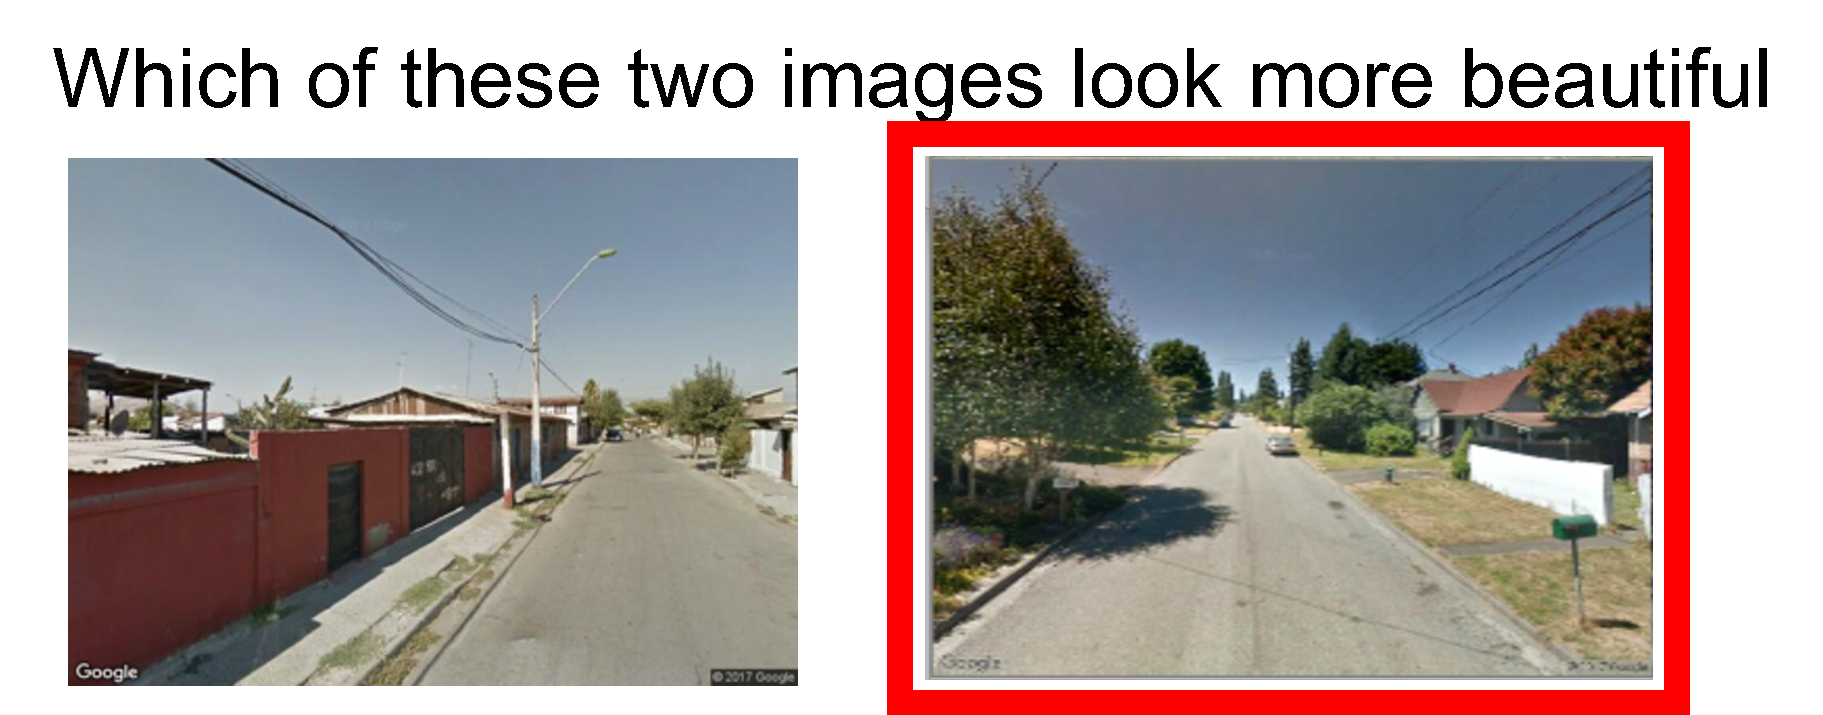
\includegraphics[width=\columnwidth]{Pairwise.pdf}
   \caption{Example of a paiwise comparison, where a user is asked to choose the more beautiful among the two.}
   \label{fig:pairwise}
\end{figure}

We start with the  Place Pulse dataset that contains 110k Google Street Views across 56 cities across 28 countries around the world~\cite{dubey2016deep}. The voting on these scenes is taken in the form of a gamified interface, where two random images from this set are shown, and the participant is asked to choose the more beautiful of the two. The interface looks similar to Figure \ref{fig:pairwise}, where by one would preferentially end up choosing the image on the right, due to its objectively superior aesthetics as compared to the one on the left. Over the course of time, they gather votes on more than 1.2 million pairwise comparisons, distributed  across 110k images, given by more than 81k volunteers from 162 countries, with a good mix of people residing in both developed and developing countries.
The pictures were labelled by volunteers through an ad-hoc crowdsourcing website\footnote{\url{http://pulse.media.mit.edu}}. Volunteers were shown random pairs of images and asked to select which scene looked more beautiful, safe, lively, boring, wealthy, and depressing.  To our knowledge, no independent systematic analysis of the biases of Place Pulse has been conducted yet. However, it is reasonable to expect that representation biases are minimized by the substantial size of the dataset, the wide variety of places represented, and the diversity of gender, racial, and cultural backgrounds of the raters.
This process, still does not solve the problem of obtaining an annotated dataset of beautiful and ugly looking urban neighbourhoods. For that to happen, we first need to translate these comparisons in to some form of an ordinal ranking of images.

\subsection{Partitioning the data}
To solve the problem of annotating images in terms of beauty we need to have at the very least, a sense of relative ranking in terms of most popularly voted to be beautiful to the least. This approach would not quantify beauty in the absolute sense but in terms of relative consensus, provided we have enough pair wise votes. 
 
\begin{figure}[t!]
    \centering
    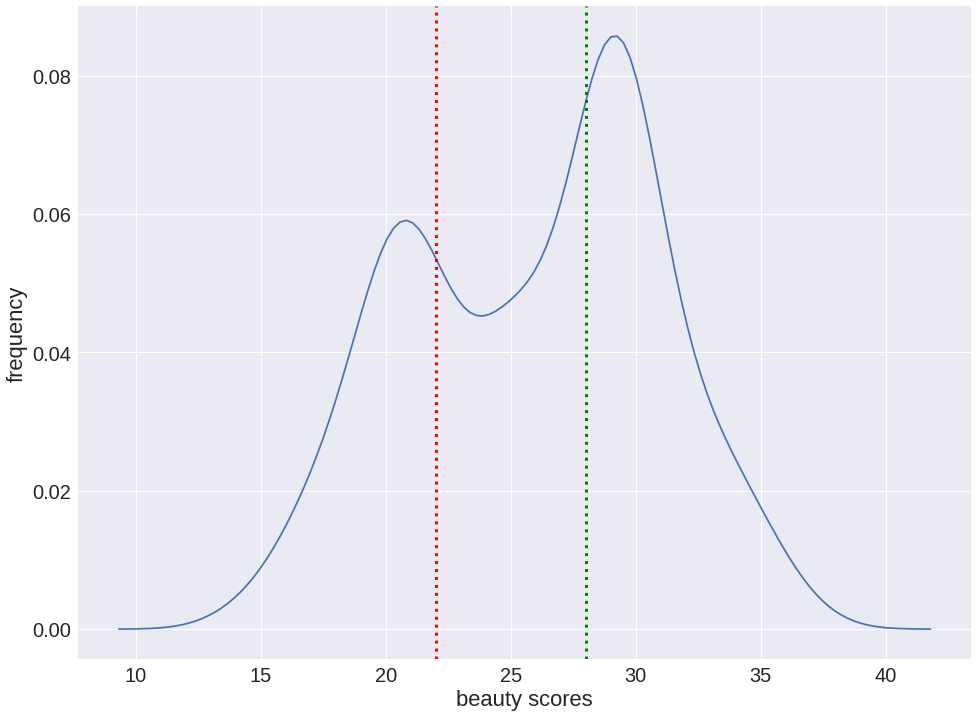
\includegraphics[width=0.7\columnwidth]{Trueskill.png}
    \caption{Frequency distribution of beauty scores. The red and green lines represent the thresholds below and above which images are considered ugly and beautiful. Conservatively, images in between are discarded.}
    \label{fig:Trueskill}
\end{figure}
To solve the problem of transforming the pairwise voting of the crowd into relative ordinal ranking, we use a popular Bayesian algorithm, used in several multiplayer gaming systems to order leader boards called TrueSkill~\cite{herbrich2007trueskill}. This algorithm works by first initializing all the players (which in our case are urban street view images) with equal ``skill'' (which in our case implies a relative sense of beauty).
The algorithm then assumes competitions among the players in a 1-on-1 fashion. In the case of our work, these competitions are the pairwise votes. Each victory results in addition of some ``skill''(beauty) in the victor player's profile (street-view image) and reduction in ``skill'' in the loser's profile. The more skillful the opponent, the higher the rewards in update of one's skill. With enough average number of competitions played by each player, a steady state order of skilled players emerges. For our dataset, we initialize all images with a ``skill'' level of 25 and a variance of 3, which signifies the uncertainty in the skill level. This uncertainity would drop, as more competitions are won or lost by any given image. For the sake of accuracy and stability, we filter only the images which have more than 8 votes on them. This reduces our usable dataset from 100k images to just over 20k. But having more than 8 votes, results in a steady state bi-modal distribution of skills as shown in Figure \ref{fig:Trueskill}. This allows us to order the streetview images in an ordinal rank based on relative beauty as seen in Fig \ref{fig:trueskill_example}. 

\begin{figure}[t!]
    \centering
    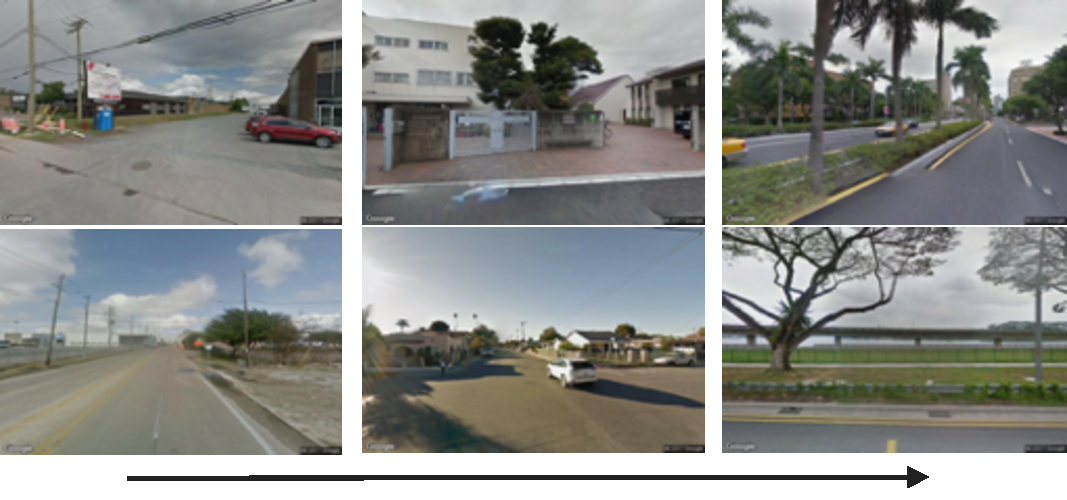
\includegraphics[width=\columnwidth]{SkillSorting.pdf}
    \caption{Sample pairs of street view images ordered by lowest final skill rating on the left to highest on the right. }
    \label{fig:trueskill_example}
\end{figure}
Despite having a consensus on the ordering of most of the images, we still end up with some images near the initialized skill level of 25. This means the skills of these images have not been decisively updated through the voting data. To work around these borderline cases, we partition the distribution of images along two margins in the trueskill space. The thresholds for partition are values less than $\mu - \sigma$ for the ugly set of images and values more than $\mu + \sigma$ for the beautiful set of images. This results in the threshold Trueskill of 22 and 28.
We select all images with a Trueskill value less than 22 and assign them to the ugly set of images. We then select all the images with the Trueskill value above 28, and assign them to the beauty bin.


\subsection{Augmenting the data}
\begin{figure}[t!]
    \centering
    \subfloat[]{
        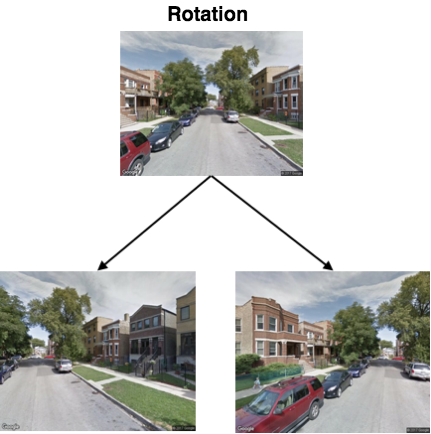
\includegraphics[width=0.5\textwidth, height = 8cm ]{rotationalSim.png}
        \label{fig:rotSim}
    }
    \subfloat[]{
        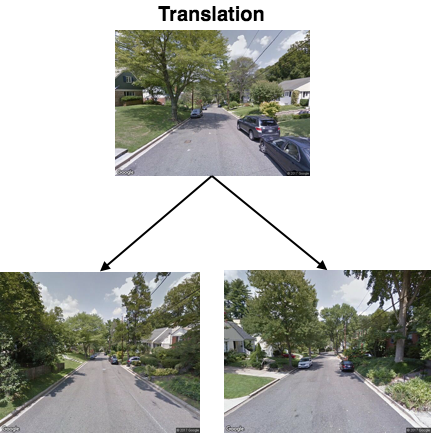
\includegraphics[width=0.5\linewidth, height = 8cm ]{transSim.png}
        \label{fig:transSim}
    }
    \caption{Two types of augmentation: (a) rotation of the Street Views camera (based on rotation); and (b) exploration of scenes at increasing distances (based on translation).}
\end{figure}
Partitioning of the data after evaluating the Trueskill scores on images is a lossy process. By the time we filter images along minimum number of votes, and based on their trueskill scores, we are left with 15,000 street-view images. It has been a well known problem in the area of deep learning, that the algorithm's performance is often limited by the amount of clean curated data available to train on. Another real danger of training on limited data is the phenomenon of overfitting. Overfitting happens when the model under consideration is reasonably complicated with millions of parameters, but the data used to train it is not sufficient to generalize the model's inference. In such cases, the model over fits to the training dataset whereby the model memorises the training data, to reduce the training error. But this model is doomed to perform poorly on a generalized set of data. To avoid this particular set of problems, I needed a way to enrich the current high confidence set of steetview images. The enrichment needs to be such that we do not add noise to the dataset, but at the same time increase the diversity of the kind of samples the model is supposed to learn. This means we need more images which are similar but not identical to the two partitions. 

The solution I develop involves two approaches. First, we feed each scene's location into the Google Streetview API to obtain the snapshots of the same location at different camera angles\footnote{Google streetview API allows the users to set the bearing and heading of the mast camera, used to acquire the image} (i.e., at $\theta \in {-30^{\circ}, -15^{\circ} , 15^{\circ} , 30^{\circ} }$). We assume that any image taken as a variant of a beautiful image at different angles of rotations can safely inherit the label of ``beauty'' since the field of view only changes by $+- 30^\circ $. With this simple (yet conservative) assumption we are able to immediately inflate our dataset by up to a factor of 5.
However, the resulting dataset is still too small for robust training. Therefore, again, we feed each scene's location into the Google Streetview API, but we now do so to obtain other scenes at  distance $d \in \{10,20,40,60\}$ meters.  This will greatly expand our set of scenes, but it might do so at the price of introducing scenes whose beauty scores have little to do with the original scene's. 
This addition of noise may have an adverse effect on the deep learning algorithm's performance for detecting beauty. 
This addition of translational data, could be done using some heuristics. Imagine a scene $I$ translated in space by 10 meters. The newly acquired scene $I_{10}$, may be useful in our augmented dataset \textit{iff} the translated scene $I_{10}$ is visually ``similar'' to the original scene $I$. The same heuristic metric can be used to either accept or reject any image $I_{m}$ translated by $m$ meters, into the augmented dataset. 
For this heuristic test to work, we first need to device a way to compute the ``similarity'' measure between two images $I$ and $I_{m}$. 
One well known way to evaluate image ``similarity'' is by represent them in a high dimensional features space, obtained from a pre-trained neural network~\cite{zhang2018unreasonable}. This is done by using the activations of a the last but two (or last but one) fully connected layer of a trained convolutional neural network during a forward pass~\cite{babenko2015aggregating,Lin_2015_CVPR_Workshops,varga2016fast} as features of the image. These activations are then treated as vectors in $R^N$ euclidean space, such that they follow the distance and angle metrics. This allows comparison of images along a similarity metric simply by comparing the cosine distances or Euclidean distance between their feature vectors. For the sake of similarity of application, we use the best performance version of a pre-trainied PlacesNet deep learning model~\cite{zhou2014learning}. PlasesNet was trained on streetview images, and is trained with the end goal of classifying streetview images into scene types, such as a beach, highway, garden etc. 

We represent the two scenes $I$ and $I_m$ with visual features derived from the \textsl{FC7} layer of PlacesNet and compute the similarity between the two corresponding feature vectors using L2 norm. 
For all scenes $I_m$ at increasing distance $m \in \{10,20,40,60\}$ meters,  we take only those whose similarity scores with the original scene is above a threshold. In a conservative fashion, we choose that threshold to be the median similarity between rotated and original scenes (those of the first augmentation step). This assures that the translated images are at the very least as similar to the original, as the rotated images.


\subsubsection{Which scenes are more suitable for translation?}
\begin{figure}[t!]
    \centering
    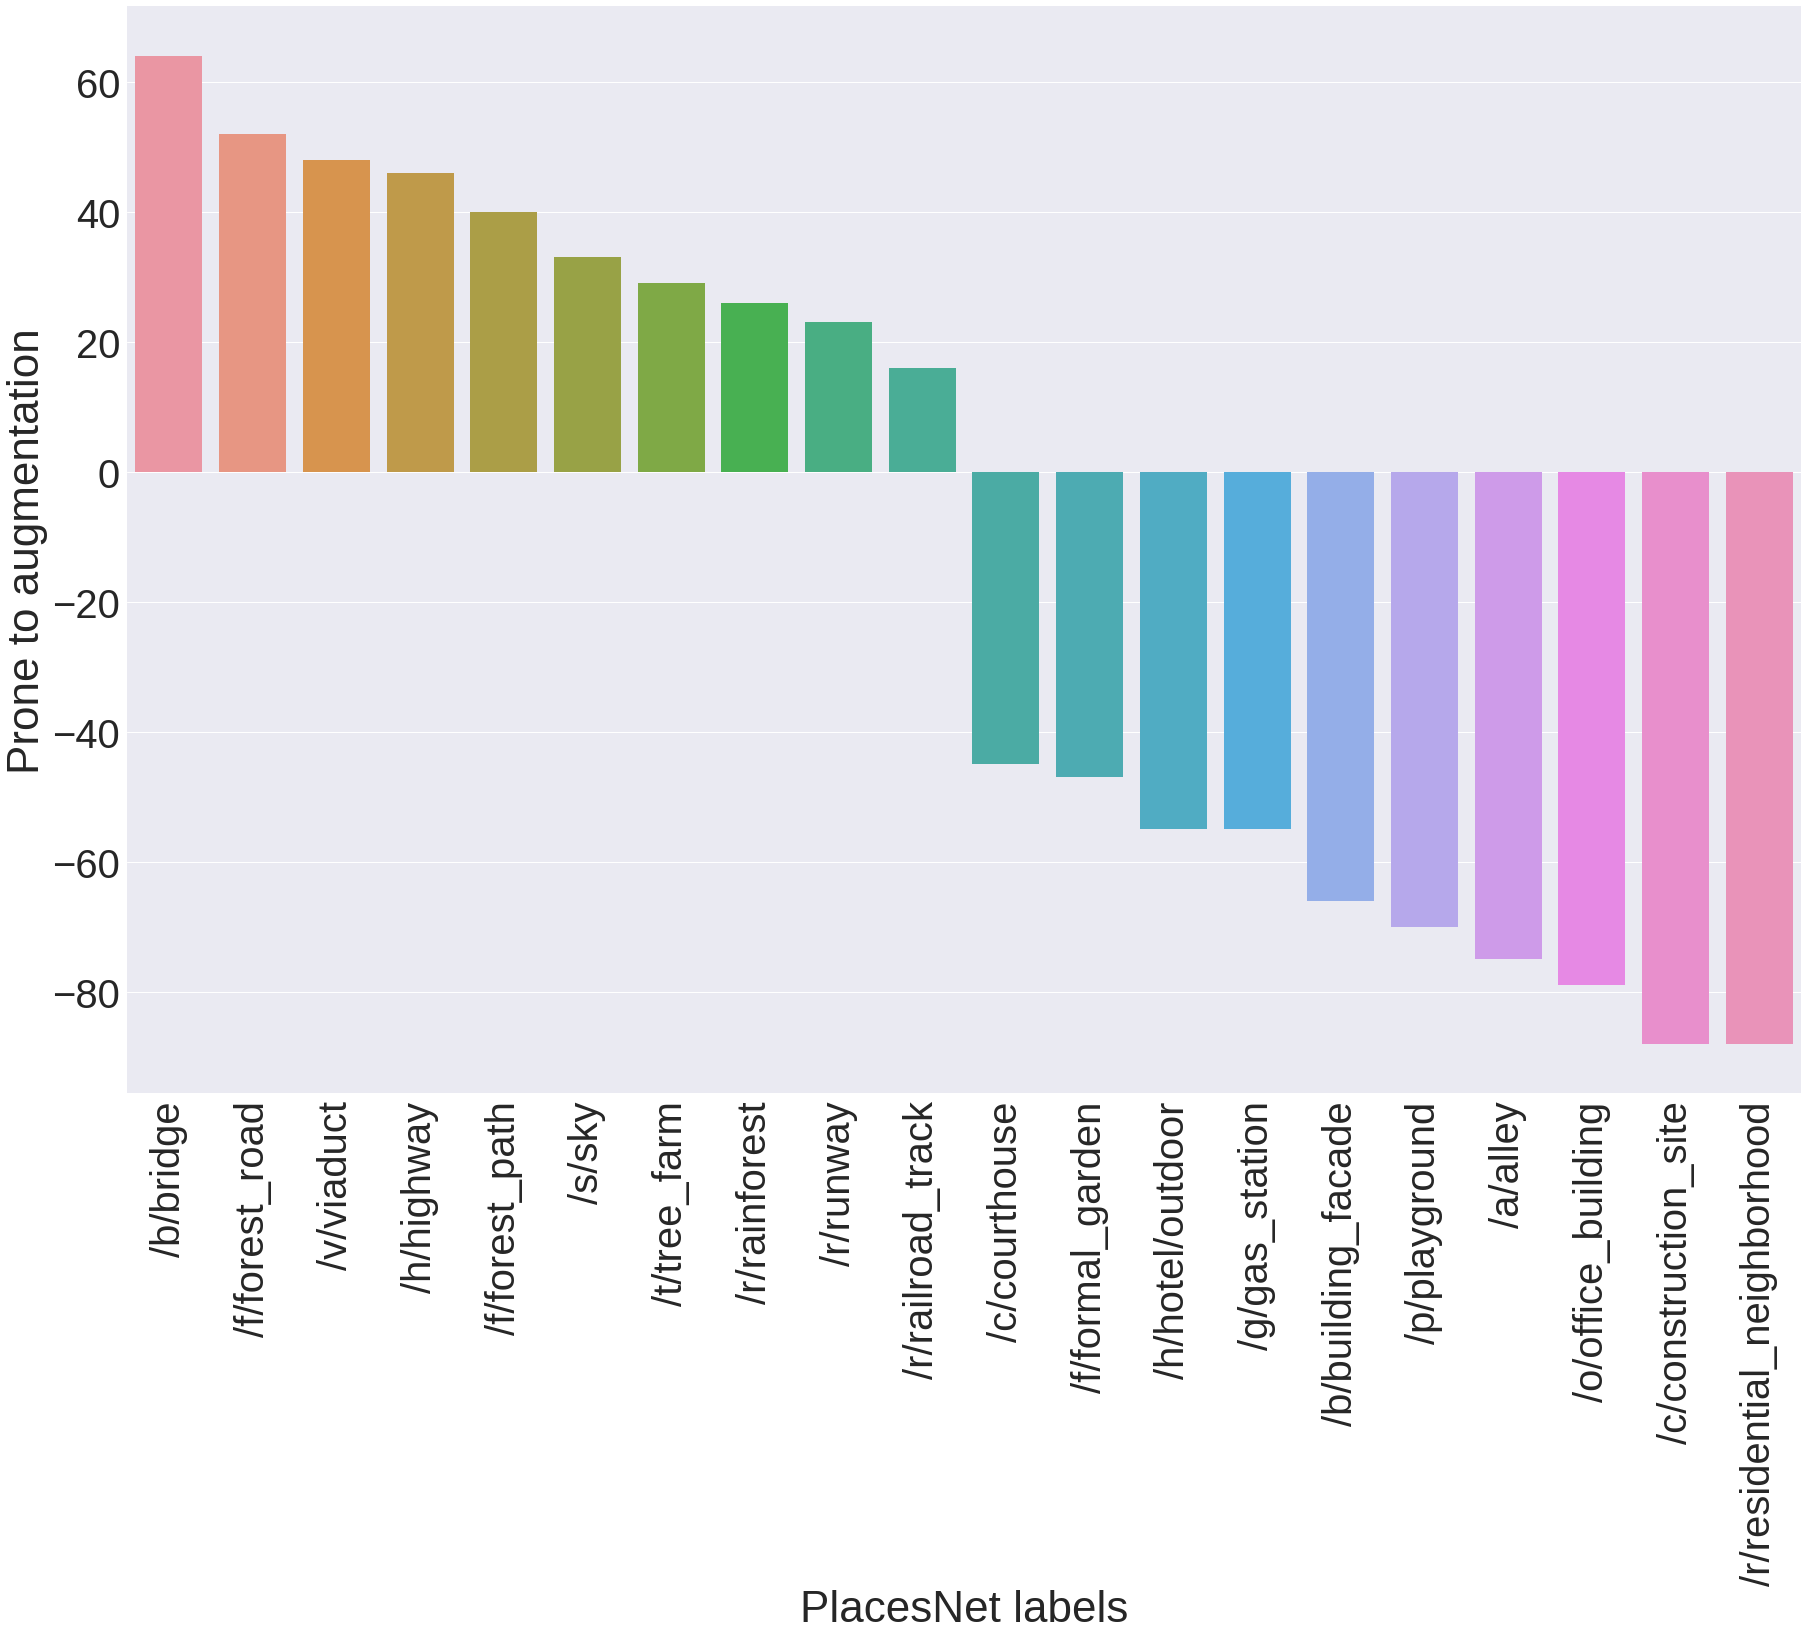
\includegraphics[width=\columnwidth]{SimilarityPlacesPrevalence.png}
    \caption{The types of scene that have greater propensity to be correctly augmented with similar scenes at increasing distances.}
    \label{fig:augmentationSimilarity}
\end{figure}
To make sure this additional augmentation has not introduced any unwanted noise, we consider  two sets of scenes: one containing those that have been taken during this last step, i.e., the one with high similarity to the original scenes:(\emph{taken-set}), and the other containing those that have been filtered away because their similarity metric went above the threshold:(\emph{filtered-set}). Each scene is then scored with PlacesNet~\cite{zhou2014learning} and is represented with the five most confident scene labels, as per the original output of the model . We then aggregate labels at set level by computing each label's frequency on the \emph{taken-set} 
and on the \emph{filtered-set}. Finally, we characterize each label's propensity to be correctly augmented as:
\begin{equation}
    \textrm{prone}(label)= fr(label,\textrm{\emph{taken-set}}) - fr(label,\textrm{\emph{filtered-set}})
\end{equation} 
This reflects the extent to which a scene with a given scene label is prone to be augmented or not, according to our decided threshold method. From Figure~\ref{fig:augmentationSimilarity}, we find that, as one would expect, scenes that contain high amount of visual continuity over long stretches such as highways, fields and bridges can be augmented at increasing distances while still showing resemblances to the original scene. By contrast, scenes that contain peculiar features with smaller continuity such as gardens, residential neighbourhoods, plazas, and skyscrapers cannot be easily augmented. These scene types also tend to be found in high density parts of the city in which visual diversity within short distances might well be experienced. 

\section{Building a beauty Classifier}

\begin{figure*}[t!]
    \centering
    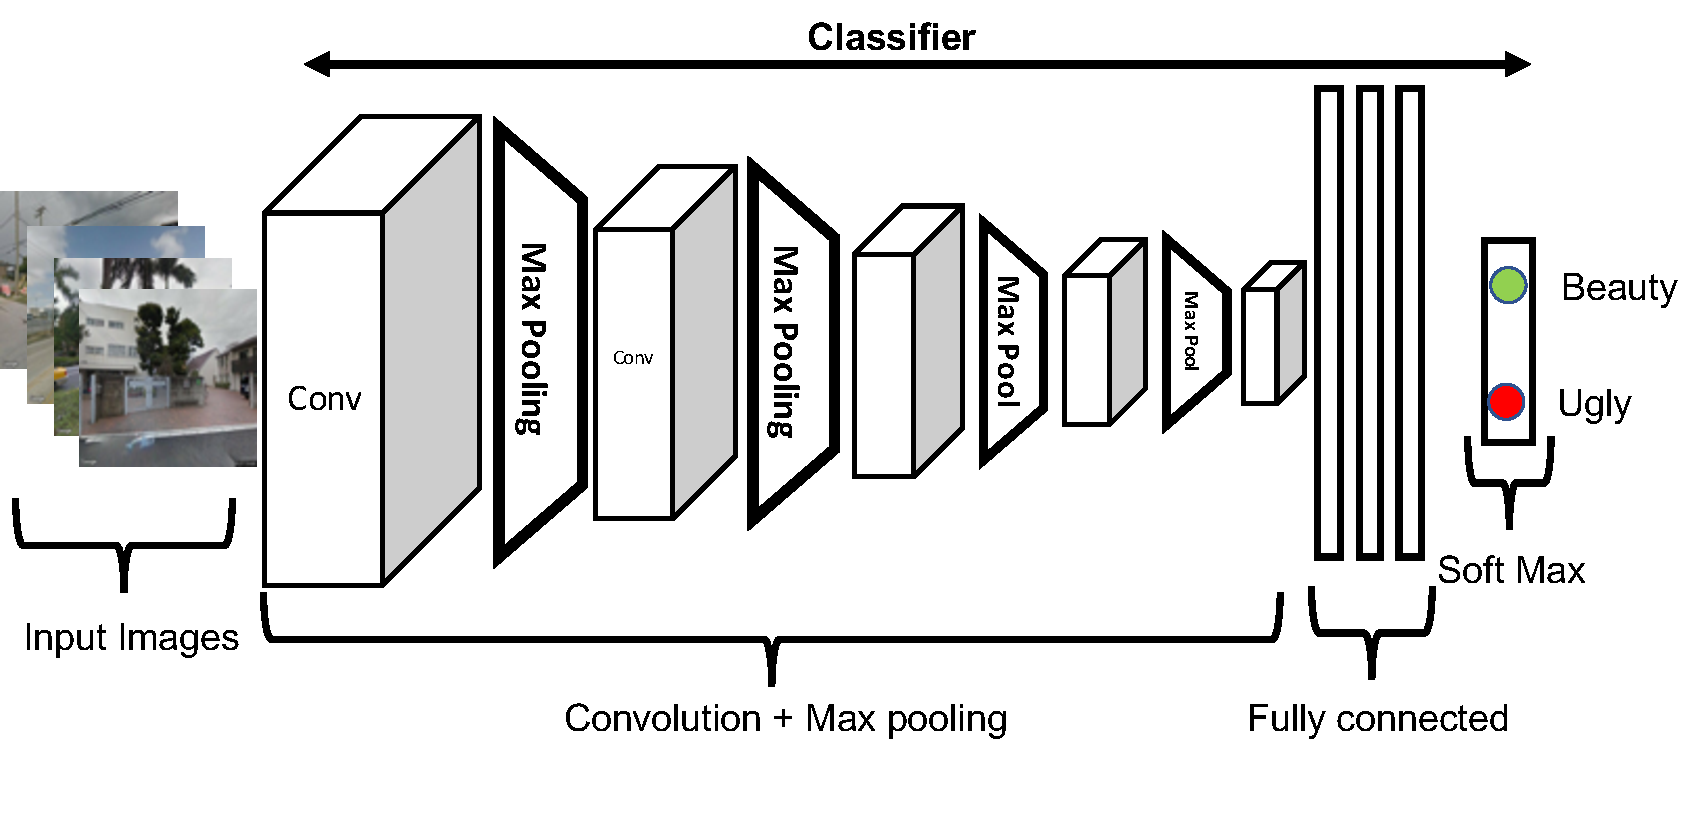
\includegraphics[width=\columnwidth]{Classifier_arch.pdf}
    \caption{}
    \label{fig:classifier_arch}
\end{figure*}

\label{sec:framework}
\begin{table}[ht!]
    \centering
    \begin{tabular}{|c|c|}
        \hline
        \textbf{Augmentation} & \textbf{Accuracy (Percentage)}\\
        \hline
        None & 63 \\
        \hline
        Rotation  & 68 \\
        \hline
        Rotation + Translation  & 64 \\
        \hline
        Rotation + Conservative Translation & 73.5 \\
        \hline
    \end{tabular}
    \caption{Percentage accuracy for our beauty classifier trained on differently augmented sets of  urban scenes.}
    \label{tab:classifier}
    \vspace{-10mm}
\end{table}

Having this highly curated set of labeled urban scenes, we are now ready to train classifier $C$ with labels reflecting our beauty assessments. The challenge here is to understand if a deep learning model is able to capture the essence of something as subjective as \textbf{perceived urban beauty}.

As for classifier $C$, we use the CaffeNet architecture, a modified version of AlexNet~\cite{krizhevsky2012imagenet,szegedy2015going} as seen in Figure \ref{fig:classifier_arch}. This has a conventional architecture with 5 convolutional layers; interleaved with  max pooling and normalization layers; and terminated by: \emph{(i)} three 4096 dimensional fully connected layers interleaved with dropout layers~\cite{srivastava2014dropout} (the dropout ratio is set to 0.5 to prevent over-fitting), and \emph{(ii)} by a Softmax layer that classifies the input image into one of two classes of beautiful(1) and ugly(0). The network is trained for 30,000 epochs with ADAM optimizer\footnote{The best performance model can be found here: \url{https://dataverse.harvard.edu/dataset.xhtml?persistentId=doi:10.7910/DVN/ATXYTP}}

Having $C$ at hand, we now turn to training it. The training is done on a 70\% split of the data, and the testing on the remaining 30\%. All this is done on increasingly augmented sets of data. We start from our 15k images and progressively augment them with  the snapshots obtained with the 5-angle camera rotations, and then with the exploration of scenes at increasing distance $d \in \{10,20,40,60\}$ meters. The idea behind this data augmentation is that the model's accuracy should increase with increasing levels of augmentation. Indeed it does (Table~\ref{tab:classifier}): it goes from 63\% on the set of original scenes to a value as high as  73.5\% on the set of fully augmented scenes, which is a notable increase in accuracy for this type of classification tasks. Furthermore, our results match previous ones: for example,  Dubey et.al's~\cite{dubey2016deep}  model showed an accuracy of 70\%, which is comparable to ours. 
The comparable, and at times better, performance of this classifier with respect to the baseline shows that 1) the notion of subjective beauty can be learn't from a crowd's participation and 2) the novel method of augmenting data, can make deep learning better accessible when the data is sparse and of urban nature.

\section{Implication of a beauty classifier}
In this chapter \textbf{RQ4} aimed at investigating the possibility of modelling subjective perceptions of aesthetics in real world, using the opinions of a vast disconnected crowd.
 
We found that using a crowd based pooling of opinions about urban beauty, we can make measurable progress towards quantifying the aesthetic in the context of urban scenes. This too can be done at scale, with a proposed novel way of augmenting sparse datasets. However, just capturing the perception is not enough to make any meaningful contribution towards the urban science. 
A lot of work has been put in understanding the impact of the urban aesthetic of citizen's health, well being, economical vitality etc. The unanimous consensus points to the fact that cites and their compositions deeply affect our health and well being. 
At this juncture it is more valuable to first understand if the notion of beauty captured by our deep learning model is analogues to that perceived by real humans. If that is indeed the case, it is worth understanding what aspects of an urban scene are predictive of the perceived beauty. This shall be of immense value to the practitioners of urban design, architecture and urban activism.

In the next chapter, we would explore exactly that. The guiding question is, can the learnt representation of urban beauty be utilized to understand the predictive motifs of urban design for beauty? Can these insights be used in a constructive way to improve existing urban scenes ? And finally, can such a framework be useful to the cause of urban design ? 



\chapter{Perceptions in real spaces}

% **************************** Define Graphics Path **************************

\graphicspath{{Chapter5/plots/} {Chapter5/plots/examples/}}
    
There has been an explosive growth of deep learning technologies and their competency in the recent years, resulting in cross disciplinary use cases of deep learning enabled tools. In the area of computer vision and urban informatics, deep learning techniques have recently been used to predict whether urban scenes are likely to be considered beautiful, and it turns out that these techniques do so quite accurately. However, the technology falls short when it comes to generating actionable insights for AI assisted urban design. To support urban interventions, one needs to go beyond \emph{predicting} beauty, and tackle the challenge of \emph{recreating} beauty and \emph{explaining} the predictors of beauty.  Unfortunately, deep learning techniques have not been designed with that challenge in mind. Given their ``black-box nature'', they cannot even explain why a scene has been predicted to be beautiful. To partly fix that, we propose a deep learning framework (which we name  FaceLift) that is able to both \emph{beautify} existing Google Street views and \emph{explain} which urban elements make those transformed scenes beautiful. To quantitatively evaluate our framework, we cannot resort to any existing metric (as the research problem at hand has never been faced before) and need to  formulate new ones. These new metrics should ideally capture the presence (or absence) of elements that make urban spaces great. Upon a review of the urban planning literature, we identify four main metrics: walkability, green, openness, and visual complexity.  For all the four metrics, the beautified scenes meet the expectations set by the literature on what great spaces tend to be made of. The transformations and their explanations are also found to be very helpful in understanding interventions for beautification, which we validate using a 20-participant expert survey. These results suggest that, in the future, as our framework's components are further researched and become better and more sophisticated, it is not hard to imagine technologies that will be able to accurately and efficiently support architects and planners in the design of the spaces we intuitively love.


\section{Introduction}


Whether a street is considered beautiful is subjective, yet research has shown that there are specific urban elements that are universally considered beautiful: from greenery, to small streets, to memorable spaces~\cite{alexander1977pattern, quercia2014aesthetic,salesses2013collaborative}. These elements are those that contribute to the creation of what the urban sociologist Jane Jacobs called `urban vitality'~\cite{jacobs1961death}. 


Given that, it comes as no surprise that computer vision techniques can automatically analyse pictures of urban scenes and accurately determine the extent to which these scenes are, \emph{on average}, considered beautiful.  Deep learning has greatly contributed to increase these techniques' accuracy~\cite{dubey2016deep}.

However, urban planners and architects are interested in urban interventions and, as such, they wish to go beyond technologies that are only able to predict beauty scores. These interests stem from the fact that the spaces we live in can be linked with several aspects of human life such as mental health\cite{seresinhe2015quantifying}, inequality \cite{salesses2013collaborative} or cultural shifts \cite{10.3389/fphy.2018.00027}. They often called for technologies that would make easier to recreate beauty in urban design~\cite{de2008architecture}. Deep learning, by itself, is not fit for purpose. It is not meant to recreate beautiful scenes, not least because it cannot provide any explanation on why a scene is beautiful. 


To partly fix that, we propose a deep learning framework (which we name  FaceLift) that is able to both \emph{generate} a beautiful scene (or, better, \emph{beautify} an existing scene) and \emph{explain} why that scene is beautiful. This opens up a possibility of using technology in urban planning efforts like decision making based of subjective opinions, participatory urban planning and promotion of restorative urban design such as green spaces and walkable areas.  Through this work, we make two main contributions:

\begin{itemize}
    \item We propose a deep learning framework that is able to learn whether Google Street views are beautiful or not, and that, based on that training, is able to both \emph{beautify} existing views and \emph{explain} which urban elements  make these views beautiful (Section~\ref{sec:framework}). 
    
    \item We quantitatively evaluate whether the framework is able to actually produce beautified scenes (Section~\ref{sec:evaluation}). We do so by proposing a family of four urban design metrics that we have formulated based on a thorough review of the literature in urban planning. For all these four metrics, the framework passes with flying colors: with minimal interventions, beautified scenes are twice as walkable as the original scenes, for example. Also, after building an interactive tool with ``FaceLifted'' scenes in Boston and presenting it to twenty experts in architecture,  we found that the majority of them agreed on three main areas of our work's impact: decision making, participatory urbanism, and promotion of restorative spaces among the general public. 
    
    %\item We find that a vast majority of participants see a general potential for the technology: 85\% of expert participants stated that it was probably better than existing tools used for \textit{``Participatory approaches on urban planning''}. 70\% expressed the  same opinions about its utilization for \textit{``decision making''}, also 70\% saw potential in its ability to \textit{``promote green cities''}.  
\end{itemize}
For sake of brevity, we will use the term 'Urban Scene` through out the paper to address an arbitrary Google Street View image. The image is fetched from a particular latitude and longitude point on the map. 
In the rest of the paper we explore related literature across various tracks of urban perceptions and urban beauty in Section \ref{sec:related}. We then describe in detail the Facelift framework in Section \ref{sec:framework}. The evaluation of the framework is described in detail in Section \ref{sec:evaluation} We conclude by pointing out some limitations and biases that might well guide future work (Section~\ref{sec:discussion}).






\section{Related Work}
\label{sec:related}
%\ns{This needs more work.}
Previous work has focused on collecting ground truth data about how people perceive urban spaces, on predicting urban qualities from visual data, and on generating synthetic images that enhance a given quality (e.g., beauty). 


\mbox{}\\
\noindent
\textbf{Ground truth of urban perceptions.} So far the most detailed studies of perceptions of urban environments and their visual appearance have relied on personal interviews and observation of city streets: for example, some researchers relied on annotations of video recordings by experts~\cite{sampson04seeing}, while others have used participant ratings of simulated (rather than existing) street scenes~\cite{lindal2012}. The web has recently been used to survey a large number of individuals. Place Pulse is a website that asks a series of binary perception questions (such as `Which place looks safer [between the two]?') across a large number of geo-tagged images~\cite{salesses2013collaborative}. In a similar way, Quercia \emph{et al.} collected pairwise judgments about the extent to which urban scenes are considered quiet, beautiful and happy~\cite{quercia2014aesthetic}. They were then able to analyze the scenes together with their ratings using image-processing tools, and found that the amount of greenery in any given scene was associated with all three attributes and that cars and fortress-like buildings were associated with sadness. Taken all together, their results pointed in the same direction: urban elements that hinder social interactions were undesirable, while elements that increase interactions were the ones that should be integrated by urban planners to retrofit cities for greater happiness. 

\mbox{}\\
\noindent
\textbf{Deep learning and the city.} Computer vision techniques have increasingly become more sophisticated. Deep learning techniques, in particular, have been recently used to accurately predict urban beauty~\cite{dubey2016deep,seresinhe2017using}, urban change~\cite{naik2017computer}, and even crime~\cite{DeNadai16}. These works also did some interesting analysis of the data to understand how safety, depression, beauty and other such dimensions are perceived across urban spaces.  \cite{dubey2016deep} also utilized deep learning methods to train models capable of comparing two urban images for their perception values in terms of beauty et.al. However even these works did not dive into the reasoning aspect of these models.

\mbox{}\\
\noindent
\textbf{Generative models.} Deep learning has recently been used not only to analyze existing images but also to generate new ones. n the past couple of years, there have been papers which exploit generative version of neural nets to delve into the aspects of explainability. Nguyen \emph{et al.}~\cite{nguyen2016synthesizing} used generative networks to create a natural-looking image that maximizes a specific neuron. In theory, the resulting image is the one that ``best activates'' the neuron under consideration (e.g., that associated with urban beauty). In practice, it is still a synthetic template that needs further processing to look realistic. \mbox{} \\

\mbox{}
To sum up, a lot of work has gone into collecting ground truth data about how people tend to perceive urban spaces, and into building accurate predictions models of urban qualities. However,  little work has gone into models that generate realistic urban scenes and that offer human-interpretable explanations of what they generate. 




\section{FaceLift Framework}
\label{sec:framework}

\begin{table}[t]
    \resizebox{0.7\linewidth}{!}{
        \begin{tabular}{l|p{8cm}}
            \textbf{Symbol} & \textbf{Meaning}\\
            $I_i$    & Original urban scene \\
            $Y$    & Set of annotation classes for urban scenes (e.g., beautiful, ugly)\\
            $y_i$    & Annotation class in $Y$ (e.g., beautiful) \\
            $\hat{I_j}$ & Template scene (synthetic image) \\
            $I'$ & Target Image \\
            $C$ & Beauty Classifier \\
            %$R$ & Images acquired by rotating Street view camera \\
            %$T$ & Images acquired by translating street view camera\\
            %$\rho$ & Similarity bound below which smart augmentation chooses translated images \\
            & \\
            %			\textbf{term} & \textbf{stands for}\\
            %			\textit{Template Image} $\hat{I_j}$    & A synthetic transformation of input image $I$ towards the class $y_j$ \\
            %			\textit{Target Image} $I'$    & The natural image which is most visually similar to the template image \\
            %		%	\textit{ Data Clustering}    & A process which groups images in $X$ according to visual similarity (e.g urban vs rural)\\
            %			\textit{Data Augmentation}    & A process of data expansion which looks for images taken in the surroundings of the georeferenced images in $X$\\
            %			\textit{Classifier}   & A deep-learning framework that is able to classify images into one of the classes in $Y$\\
            %			\textit{Generator} $(GAN)$    & A deep-learning based image generator \\% framework to produce images similar to the ones in  $X$\\
            %			$DGN-AM$    & A framework that, given the GAN and the Classifier, transforms an input image into the template image.\\
    \end{tabular}}
    \caption{Notations}\label{notations}
\end{table}

\begin{figure*}[ht]
    \centering
    \includegraphics[width=\linewidth]{facelift-pipeline-2x.png}
    \caption{A simplistic end to end illustration of the FaceLift framework.}
    \label{fig:framework}
\end{figure*}

%****************************************
The goal of FaceLift is to take as input a geo-located urban scene and give as output its transformed (beautified) version. 
To that end, it performs in five steps: 
\begin{itemize}
    \item \textbf{Curating urban scenes} It is common knowledge that deep learning systems need immense amount of data. In this first step we try to develop a sound framework for curating and augmenting annotated images, on which the model could be trained.
    \item \textbf{ Training a beauty classifier} To generate beauty, you first need a reliable model that could learn the representation of beauty. To achieve this, we train a deep learning model that could distinguish beautiful urban scenes from non-beautiful urban scenes. 
    \item \textbf{Generating a synthetic beautified scene} Based on the learned representation of beauty, we train a Generative model which could augment the beauty of an input urban scene. 
    \item \textbf{Retrieving a realistic beautified scene} as showcased in Figure \ref{fig:framework}, the generated images are representations of beautified input urban scene in a latent space. This latent representation needs to be transformed back to a realistic looking image, using retrieval.
    \item \textbf{Identifying the urban elements characterizing the beautified scene} In the final step, the framework explains changes introduced in the transformation process in terms of literature-driven urban design metrics, and quantifies these changes as metrics for urban beauty.
\end{itemize}
%1) curating urban scenes; 2) training a beauty classifier; 3) generating a synthetic beautified scene; 4) returning a realistic beautified scene; and 5) identifying the urban elements characterizing the beautified scene. 
%\ns{You need a bit more detail here. First sentence says what you are going to achieve. But you need to motivate why these specific five steps will achieve this goal.}


%****************************************
\subsection*{Step 1 Curating Urban Scenes}
To begin with, we need highly curated training data with labels reflecting urban beauty. We start with the  Place Pulse dataset that contains 100k Google Street Views across 56 cities around the world~\cite{dubey2016deep}. These scenes are labeled in terms of whether the corresponding places are likely to be perceived beautiful, depressing, rich, and safe. We focus only on those scenes that are labeled in terms of beauty and that have at least three judgments. This leave us with roughly  20,000 scenes. To transform judgments into beauty scores, we use the TrueSkill algorithm~\cite{herbrich2007trueskill}, which gives us a way of partitioning the scenes into two sets (Figure \ref{fig:Trueskill}): one containing beautiful scenes, and the other containing ugly scenes. The resulting set of scenes is too small for training any deep learning module without avoiding over-fitting though. As such, we need to augment such a set. 

We do so in two ways. First, we feed each scene's location into the Google Streetview API to obtain  the snapshots of the same location at different camera angles (i.e., at $\theta \in {-30^{\circ}, -15^{\circ} , 15^{\circ} , 30^{\circ} }$). However, the resulting dataset is still too small for robust training. Therefore, again, we feed each scene's location into the Google Streetview API, but now we do so to obtain other scenes at  distance $d \in \{10,20,40,60\}$ meters.  This will greatly expand our set of scenes, but it might do so at the price of introducing scenes whose beauty scores have little to do with the original scene's. To fix that, we take only the scenes that are \emph{similar} to the original one (we call this way of augmenting ``conservative translation''). To compute the similarity between a pair of scenes, we represent the two scenes with visual features derived from the FC7 layer of PlacesNet and compute the similarity between the two corresponding feature vectors~\cite{zhou2014learning}. For all scenes at increasing distance $d \in \{10,20,40,60\}$ meters,  we take only those whose similarity scores with the original scene is above a threshold. In a conservative fashion, we choose that threshold to be the median similarity between rotated and original scenes (those of the first augmentation step). 

To make sure this additional augmentation has not introduced any unwanted noise, we consider  two sets of scenes: one containing those that have been taken during this last step, i.e. the one with high similarity to the original scenes (\emph{taken-set}), and the other containing those that have been filtered away (\emph{filtered-set}). Each scene is then scored with PlacesNet~\cite{zhou2014learning} and is represented with the five most confident scene labels. We then aggregate labels at set level, by computing each label's frequency on the \emph{taken-set} %minus that on the 
and on the \emph{filtered-set}. Finally, we characterize each label's propensity to be correctly augmented as: 
$ \textrm{prone}(label)= fr(label,\textrm{\emph{taken-set}}) - fr(label,\textrm{\emph{filtered-set}}).$
This reflects the extent to which a scene with a given label is prone to be augmented or not. From Figure~\ref{fig:augmentationSimilarity}, we find that, as one would expect, scenes that contain highways, fields and bridges can be augmented at increasing distances while still showing resemblances to the original scene; by contrast, scenes that contain gardens, residential neighborhoods , plazas, and skyscrapers cannot be easily augmented, as they are often found in high density parts of the city, where there is tremendous diversity within short distances. 

%\ns{You probably want to reword this: It is amenable to augmentation, not prone to. Also why is this being done at a set level? If you always find bridges next to viaducts and viaducts next to bridges, and if your translation step moves from one to another, then the set-level score will not detect this. If instead you check whether the placesnet\_label of the translated image is the same as that of the original, then you are OK, as long as placesnet\_label can be be believed.}

\begin{figure}[t!]
    \centering
    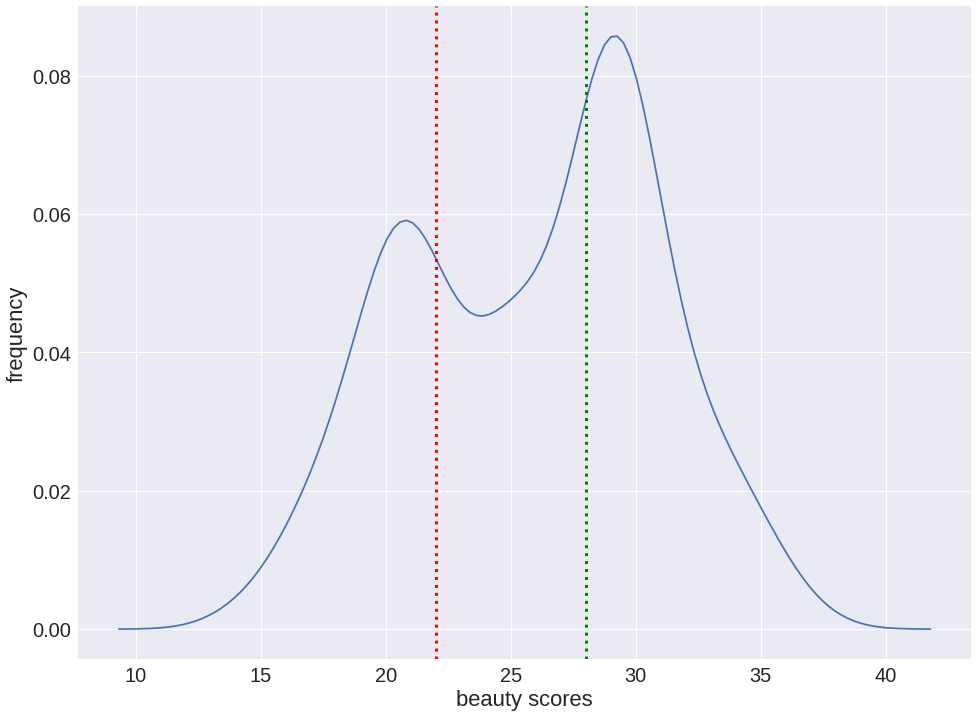
\includegraphics[width=0.7\columnwidth]{Trueskill.png}
    \caption{Frequency distribution of beauty scores. The red and green lines represent the thresholds below and above which images are considered ugly and beautiful. Conservatively, images in between are discarded.}
    \label{fig:Trueskill}
\end{figure}


\begin{figure*}[t!]
    \centering
    \hspace*{-5mm}
    \subfloat[]{
        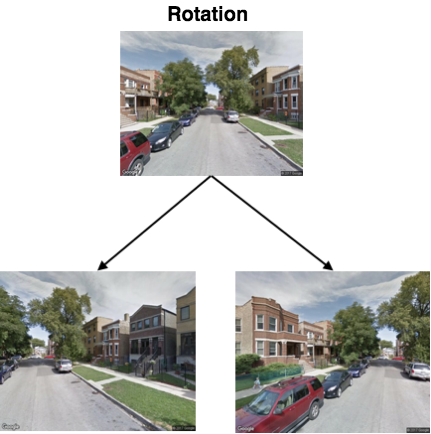
\includegraphics[width=0.5\textwidth, height = 8cm ]{rotationalSim.png}
        \label{fig:rotSim}
    }
    \subfloat[]{
        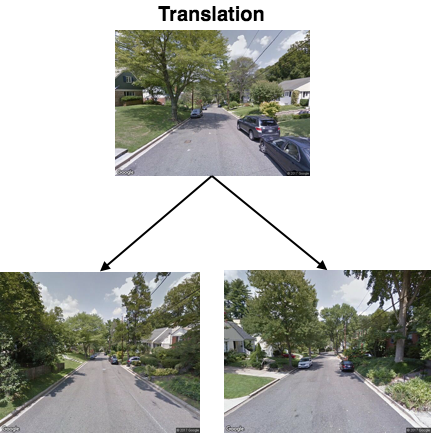
\includegraphics[width=0.5\linewidth, height = 8cm ]{transSim.png}
        \label{fig:transSim}
    }
    \vspace{-0.4cm}
    \caption{Two types of augmentation: (a) rotation of the Street Views camera (based on rotation); and (b) exploration of scenes at increasing distances (based on translation).}
    \vspace{-0.4cm}
\end{figure*}



\begin{figure}[t!]
    \centering
    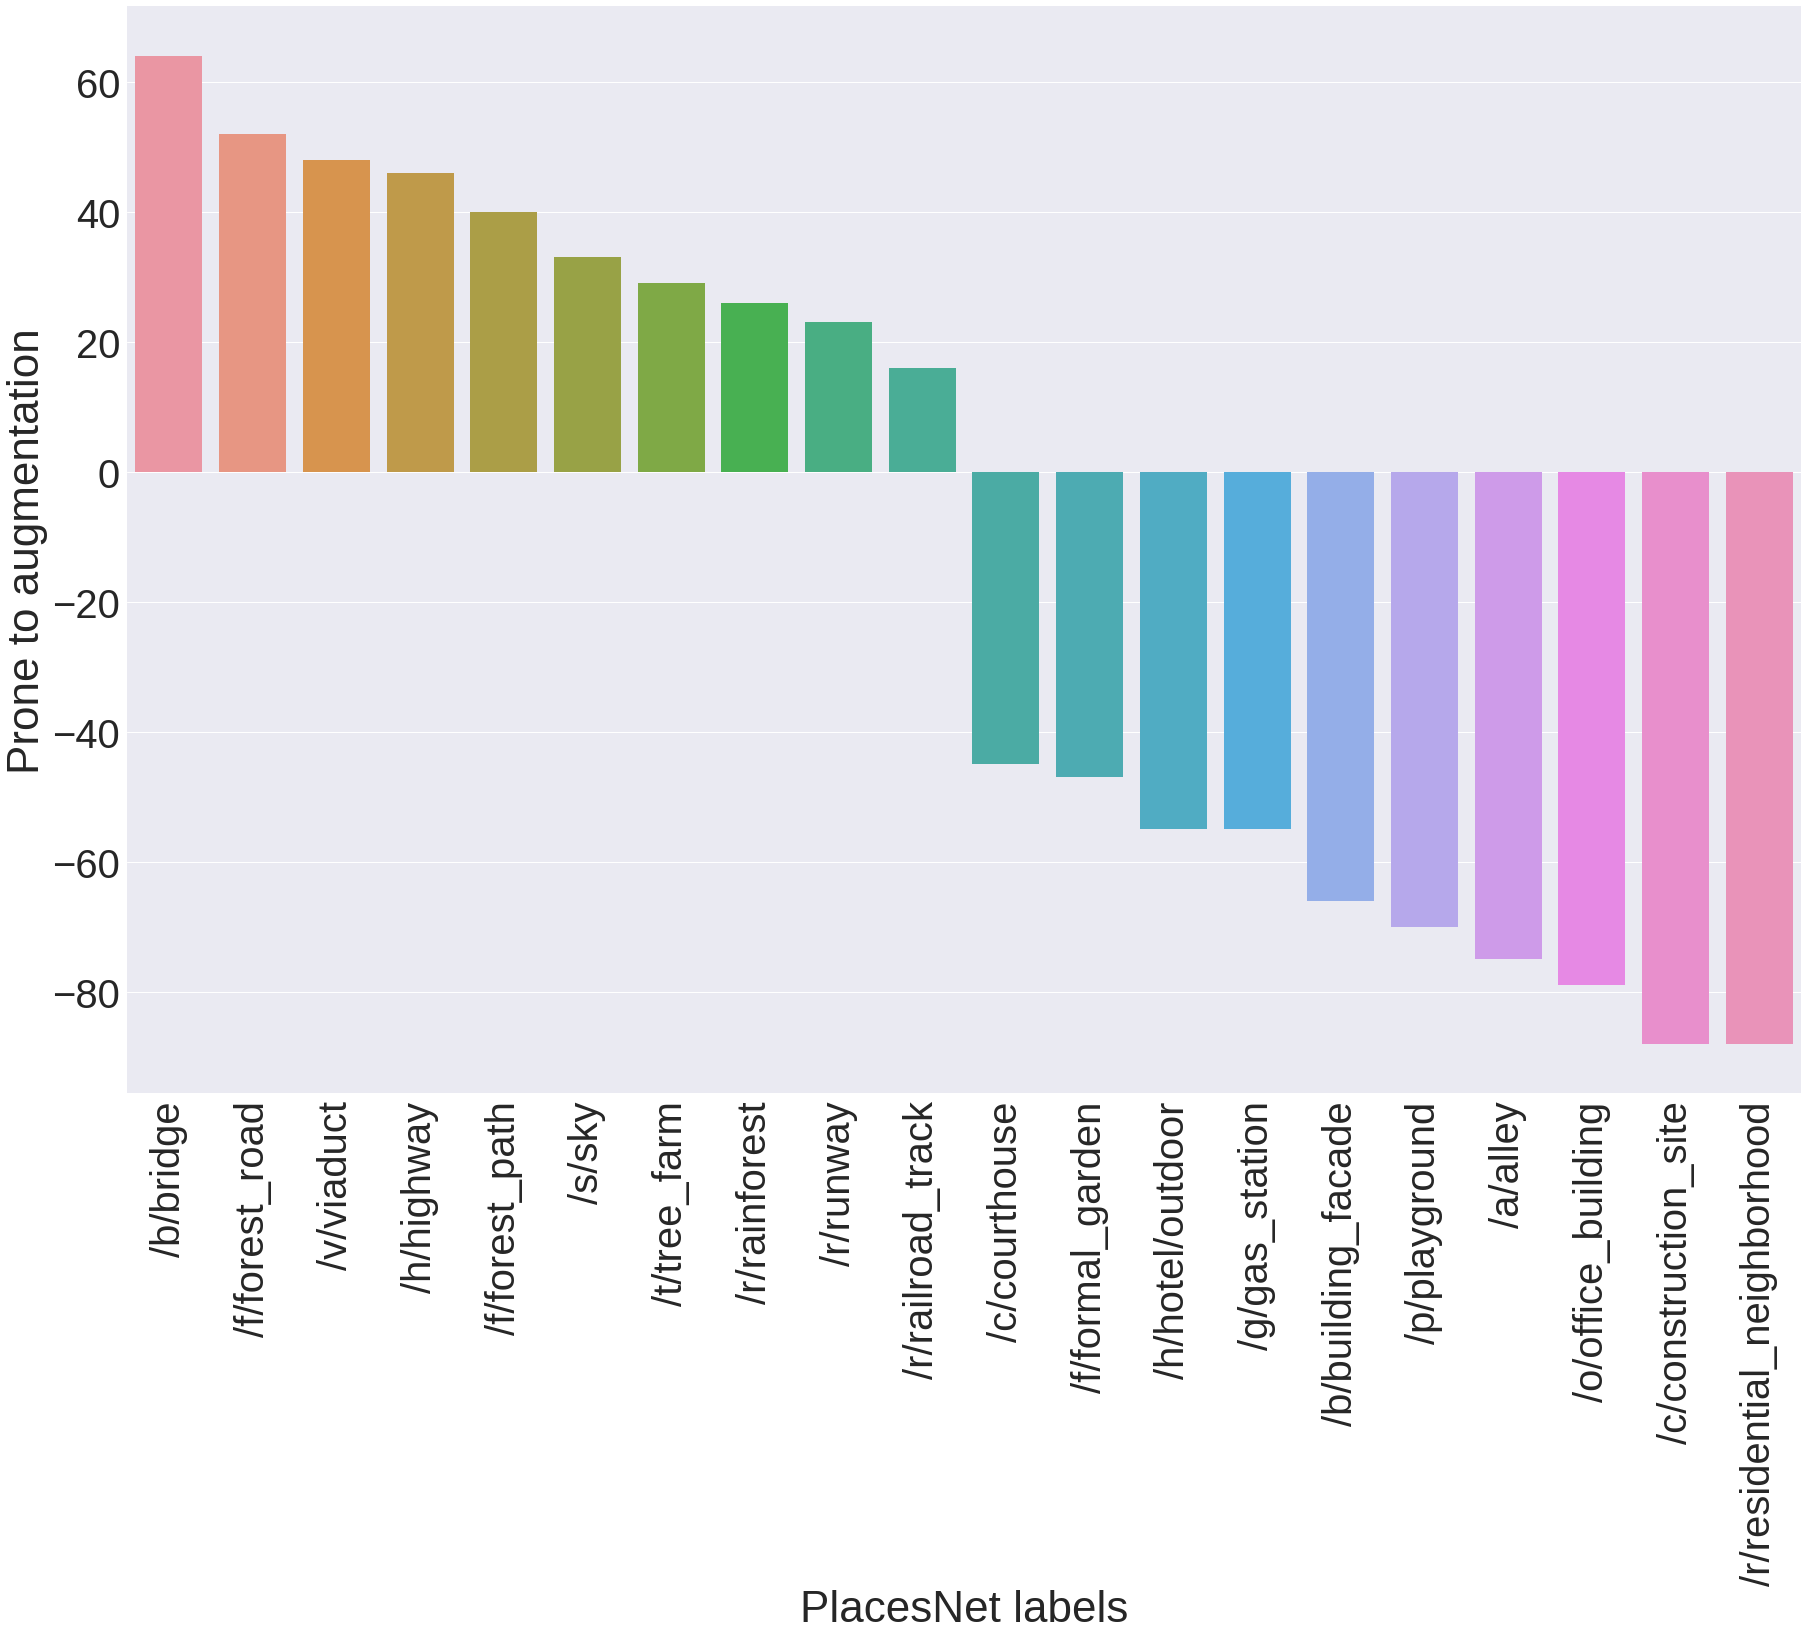
\includegraphics[width=\columnwidth]{SimilarityPlacesPrevalence.png}
    \caption{The types of scene that have greater propensity to be correctly augmented with similar scenes at increasing distances.}
    \label{fig:augmentationSimilarity}
\end{figure}




\begin{table}[t!]
    \centering
    \begin{tabular}{|c|c|}
        \hline
        \textbf{Augmentation} & \textbf{Accuracy (Percentage)}\\
        \hline
        None & 63 \\
        \hline
        Rotation  & 68 \\
        \hline
        Rotation + Translation  & 64 \\
        \hline
        Rotation + Conservative Translation & 73.5 \\
        \hline
    \end{tabular}
    \caption{Percentage accuracy for our beauty classifier trained on differently augmented sets of  urban scenes.}
    \label{tab:classifier}
    \vspace{-10mm}
\end{table}


%****************************************
\subsection*{Step 2 Training a beauty classifier}
Having this highly curated set of labeled urban scenes, we are now ready to train classifier $C$ with labels reflecting our beauty assessments. We use the CaffeNet architecture, a modified version of AlexNet~\cite{krizhevsky2012imagenet,szegedy2015going}. The training is done on a 70\% split of the data, and the testing on the remaining 30\%. All this is done on increasingly augmented sets of data. We start from our 20k images and progressively augment them with  the snapshots obtained with the 5-angle camera rotations, and then with the exploration of scenes at increasing distance $d \in \{10,20,40,60\}$ meters. The idea behind data augmentation is that accuracy would increase with it. Indeed it does (Table~\ref{tab:classifier}): it goes from 63\% on the set of original scenes to as much as 73.5\% on the set of fully augmented scenes, which is a notable increase in accuracy for such classes of classification tasks. As a baseline, we compare with the models trained by Dubey et.al in \cite{dubey2016deep} on the same seed data that we use for our pipeline. They report that their models perform at 70\% accuracy in the task of picking a beautiful image amongst any two given images. Albeit the set-up of our model is not to compare two images but just to classify a particular image in a binary class, this baseline shows that our model is showing a comparable performance in beauty classification. 
%As a baseline, we compared with the scenic-or-not model developed by Chanuki et.al \cite{seresinhe2017using}. Their model is different than ours because of the fact that their model generates scenic scores on a scale of 10, whereas ours is a binary classifier. Still for the sake of comparison, we measure the Kendall rank correlation, which is what they use for their measurements, between predicted and actual classes. Our model performs with a Kendall rank correlation of 0.43 which is comparable to their elastic net models. In so far, the facelift pipeline is agnostic of the classifier , which can be swapped out with a better performing one or with one trained for a different use case. 
%\ns{Can you cite a baseline comparison from state of the art? Less important but comment on why is accuracy the right metric? Why not precision for instance?}. 


%\begin{figure*}[h]
%	\centering
%	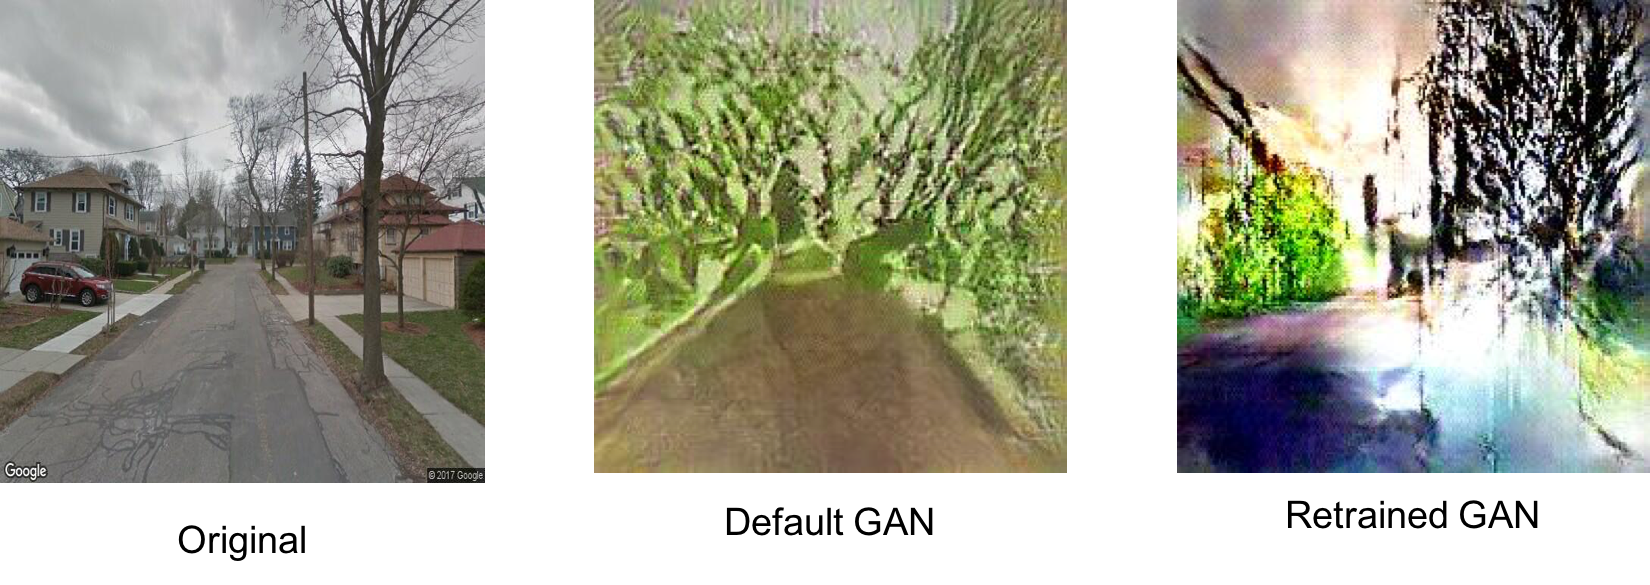
\includegraphics[width=0.5\linewidth]{Plot/GanCompare.png}
%	\caption{Comparison of using the Default ImageNet GAN against Custom trained GAN for Activation maximization. By re-training the GAN on the test dataset, we can see improvement in terms of structure and colours in the generated images}
%	\label{fig:GanComparison}
%\end{figure*}


%****************************************
\subsection*{Step 3 Generating a synthetic beautified scene}
Having this trained classifier at hand, we can then build a generator of synthetic beautified scenes. This is a model that, given the two classes ugly $y_i$ and beautiful $y_j$, transforms any original scene $I_i$ of class $y_i$ (e.g., ugly scene) into template scene $\hat{I_j}$ that maximizes class $y_j$ (e.g., beautified template scene). 

More specifically, given an input image $I_i$ known to be of class $y_i$  (e.g., ugly), our technique outputs  $\hat{I_j}$, which is a more beautiful version of it (e.g., $I_i$ is morphed  towards the average representation of a beautiful scene) while preserving $I_i$'s details. The technique does so using the ``Deep Generator Network for Activation Maximization'' (\emph{DGN-AM}) \cite{nguyen2016synthesizing}. Given an input image $I_i$, \emph{DGN-AM} iteratively re-calculates the color of $I_i$'s pixels in  a way  the output image $\hat{I_j}$  both maximizes  the  activation of neuron $y_j$ (e.g., the ``beauty neuron'') and looks ``photo realistic'',  which is done by conditioning the maximization to an ``image prior''. This is equivalent to finding the feature vector $f$ that maximizes the following expression:
\begin{equation}
\hat{I_j} =G( f ) : \underset{f}{\arg\max}(C_{j}(G(f))-\lambda||f||)
\end{equation}
where:
\begin{itemize}
    \item $G(f)$ is the image synthetically generated from the candidate feature vector $f$;
    \item $C_j(G(f))$ is the activation value of neuron $y_j$ in the scene classifier $C$ (the value to be maximized);
    \item $\lambda$ is a $L_2$ regularization term.
\end{itemize}
Here the initialization of $f$ is key. If $f$ were to be initialized with random noise, then the resulting $G(f)$ would be the average representation of category $y_j$ (of, e.g., beauty). Instead, since $f$ is initialized with $I_i$, then the resulting $G(f)$ is $I_i$'s version ``morphed to become more beautiful''. 
%Figure \ref{fig:BeautyExample} shows the activation maximization output in the center.

%****************************************
\subsection*{Step 4 Returning a realistic beautified scene}
We now have template scene $\hat{I_j}$ (which is a synthetic beautified version of original scene $I_i$) and need to retrieve a realistic looking version of it. We do so by: \emph{i)} representing each of our original scenes in Step 1 (including $\hat{I_j}$) as a 4096 dimensional feature vector derived from the FC7 layer of the PlacesNet \cite{zhou2014learning}; \emph{ii)} computing the distance (as $L_2$ Norm) between $\hat{I_j}$'s feature vector and each of the original scene's feature vector; and \emph{iii)} selecting the original scene most similar (smaller distance) to $\hat{I_j}$. This results into the selection of the beautified scene $I_j$.


%****************************************
\subsection*{Step 5 Identifying  characterizing urban elements}
Since original scene $I_i$ and beautified scene $I_j$ are real scenes and we make sure that they maintain the same structural characteristics (e.g., point of view, layout), we can easily compare them in terms of presence or absence of SegNet's and PlacesNet's labels. That is, we can determine how the original scene and its beautified version differ in terms of urban design elements. This step required us to develop metrics inspired from urban design literature, to quantify the changes in elements. A detailed description of the characterization and evaluation would follow in Section \ref{sec:evaluation}


%\begin{figure*}[h]
%	\centering
%	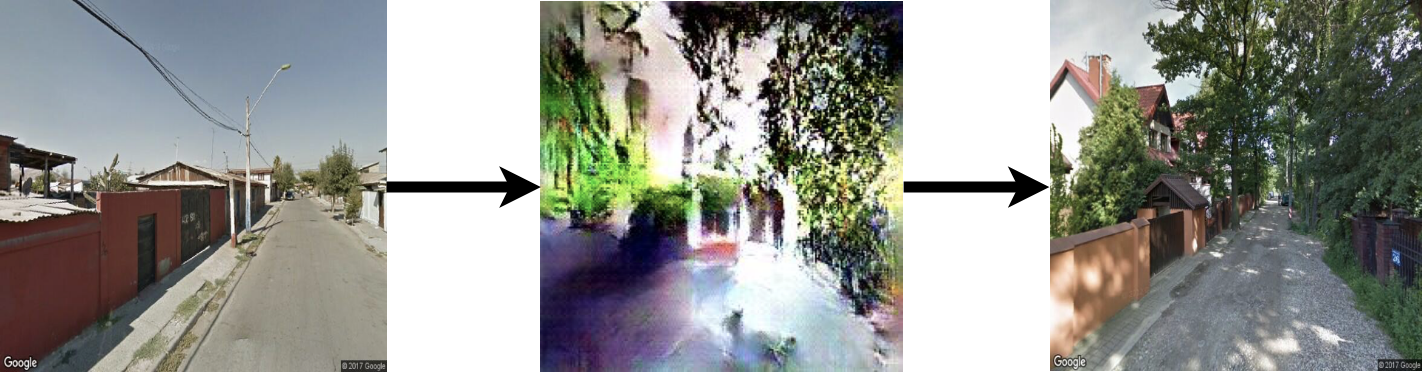
\includegraphics[width=\linewidth]{Plot/Example.png}
%	\caption{Example of ``FaceLifting''.}
%	\label{fig:BeautyExample}
%\end{figure*}


\begin{table}
    \begin{tabular}{l*3{C}@{}}
        \toprule
        & Original ($I_i$) & Latent Beauty representation ($\hat{I_j}$) & Beautified ($I_j$) \\ 
        \midrule
        & 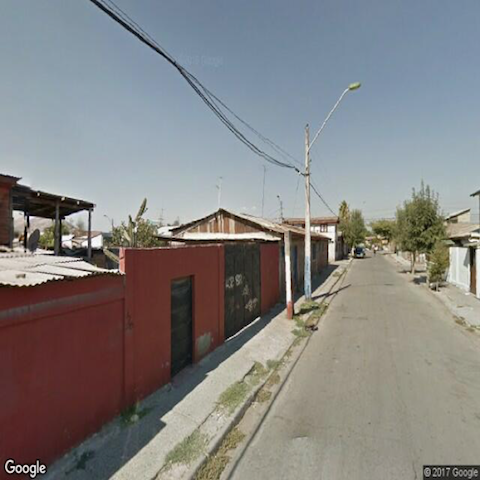
\includegraphics[width=11em]{u_9} & 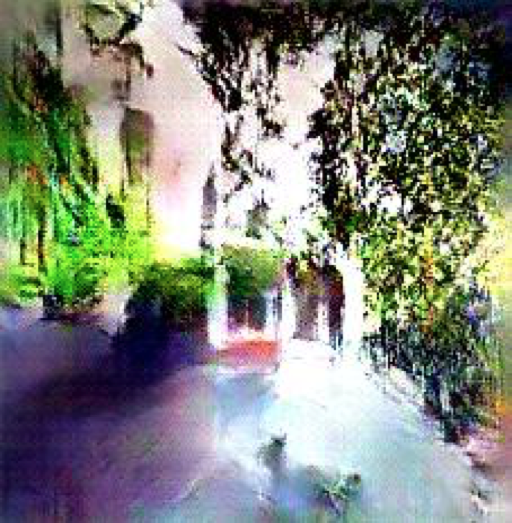
\includegraphics[width=11em]{t_9} &  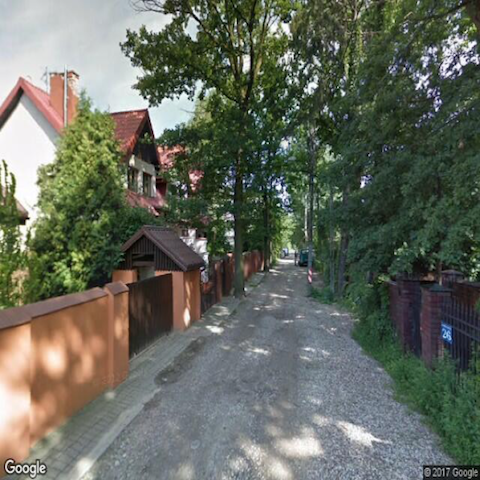
\includegraphics[width=11em]{b_9} \\ 
        & 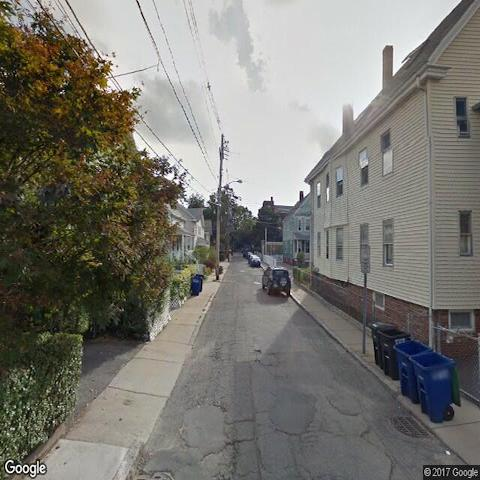
\includegraphics[width=11em]{u_4.jpeg} & 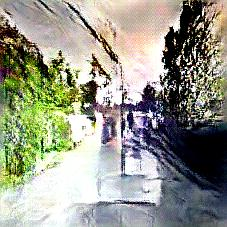
\includegraphics[width=11em]{t_4.jpeg} &  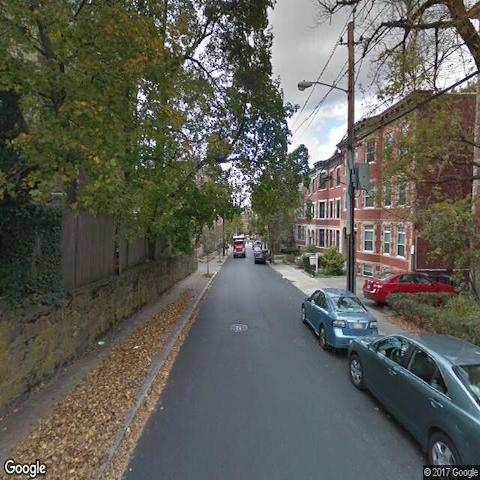
\includegraphics[width=11em]{b_4.jpeg} \\ 
        & 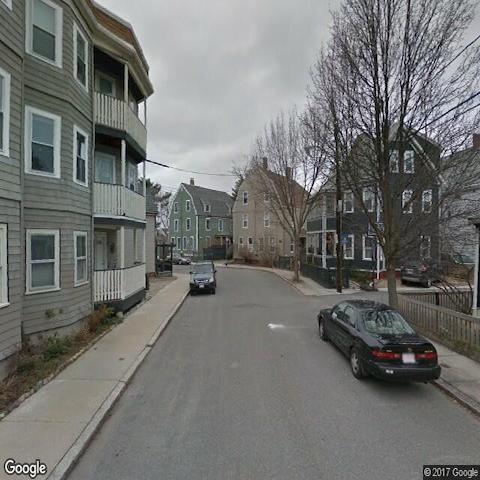
\includegraphics[width=11em]{u_5.jpeg} & 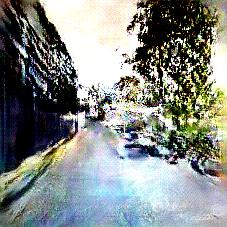
\includegraphics[width=11em]{t_5.jpeg} &  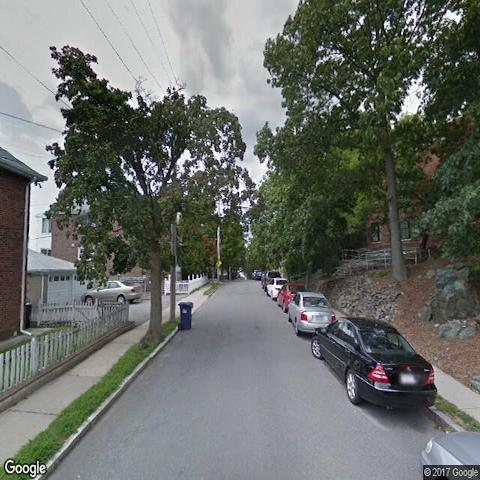
\includegraphics[width=11em]{b_5.jpeg} \\ 
        & 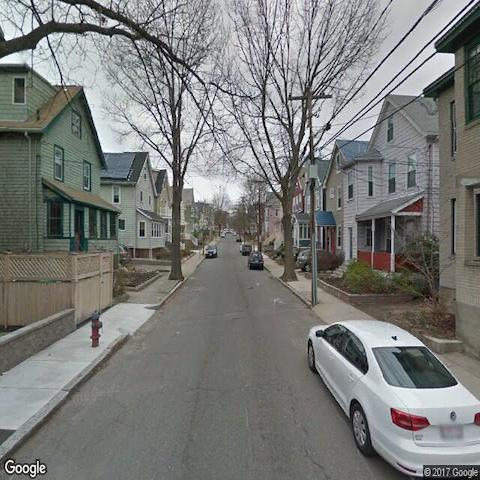
\includegraphics[width=11em]{u_7.jpeg} & 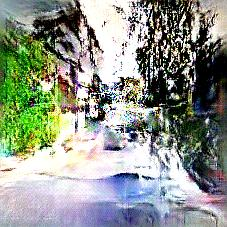
\includegraphics[width=11em]{t_7.jpeg} &  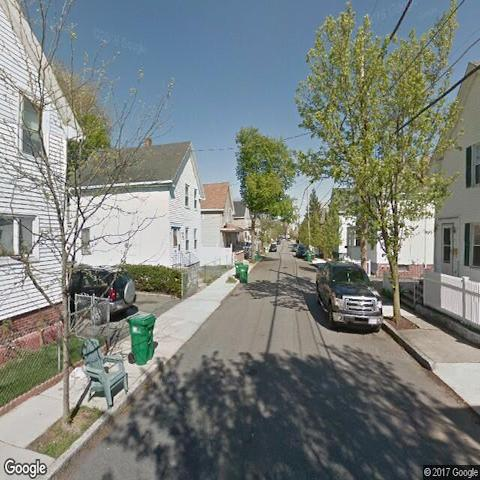
\includegraphics[width=11em]{b_7.jpeg} \\ 
        & \includegraphics[width=11em]{u_8.jpeg} & \includegraphics[width=11em]{t_8.jpeg} &  \includegraphics[width=11em]{b_8.jpeg} \\ 
        \bottomrule 
    \end{tabular}
    \caption{ The table showcases examples of the``FaceLifting'' process. It is worth observing that the process of beautification prefers greenery, narrow roads and  pavements }
    \label{fig:BeautyExample}
\end{table} 



\section{Evaluation}
\label{sec:evaluation}

The goal of FaceLift is to transform existing urban scenes into versions that: \emph{i)} people perceive more beautiful; \emph{ii)} contain urban elements typical of great urban spaces; \emph{iii)} are easy to interpret; and \emph{iv)} architects and urban planners find useful. To ascertain whether FaceLift meets that composite goal, we answer the following questions next: 

\begin{description}
    \item{\textbf{Q1}} Do individuals perceive``FaceLifted'' scenes to be beautiful?
    
    \item{\textbf{Q2}}  Does our framework produce scenes that possess urban elements typical of great spaces?
    
    \item{\textbf{Q3}}  Which urban elements are mostly associated with beautiful scenes?
    
    \item{\textbf{Q4}}  Do architects and urban planners find FaceLift useful?
    
\end{description}


\subsection*{Q1 People's perceptions of beautified scenes}
To ascertain whether FaceLifted scenes are perceived by individuals as they are supposed to, we run a crowd-sourcing experiment on Amazon Mechanical Turk.  We randomly select 200 scenes, 100 beautiful and 100 ugly  (taken at the bottom 10 and top 10 percentiles of the Trueskill's score distribution of Figure~\ref{fig:Trueskill}). Our framework then transforms each ugly scene into its beautified version, and each beautiful scene into its corresponding `uglified'. These scenes are arranged into pairs, each of which contains the original scene and its beautified or uglified version. On  Mechanical Turk, we only select verified masters for our crowd-sourcing workers (those with an approval rate above 90\% during the past 30 days), pay them \$0.1 per  task,  and ask each of them to choose the beautiful scene for given pairs.  We make sure to have at least 3 votes for each scene pair. Overall, our workers end up selecting the scenes that are actually beautiful 77.5\% of the times, suggesting that FaceLifted scenes are correctly perceived most of the times.


\subsection*{Q2 Are beautified scenes great urban spaces?}
To answer that question, we need to understand what makes a space great. After a careful review of the urban planning literature, we identify four factors~\cite{ewing2013measuring,alexander1977pattern} (summarized in Table~\ref{tab:Design_metrics}): great places mainly tend to be walkable, offer greenery, feel cozy, and be visually rich. 


\begin{table*}[h]
    \centering
    
    \resizebox{\linewidth}{!}{%
        \begin{tabular}{|c|p{10cm}|}
            \hline
            \textbf{Metric} & \textbf{Description}\\
            \hline
            Walkability  & Walkable streets increase the social capital of a place,  and they appeal to the exploring nature of the human psyche~\cite{ewing2013measuring,quercia15thedigital,speck12}.\\
            \hline
            Green Spaces & The presence of greenery has repeatedly been found to impact people's well being \cite{alexander1977pattern}. Under certain conditions, it could also promote social interactions~\cite{quercia2014aesthetic}. This suggest that not all greenery has to be considered in the same way though: dense forests or unkempt greens might well have a negative impact~\cite{jacobs1961death}. \\
            %			\hline		
            %			Landmarks & Loosing a bearing in the city is not a very pleasant experience. Hence presence of recognisable and  guiding landmarks influences the perception of an urban space \cite{ewing2013measuring}.\\
            \hline
            Privacy-Openness &  A sense of privacy (as opposed to a sense of openness) impacts a place's perception~\cite{ewing2013measuring}.\\ 
            \hline
            Visual Complexity & Visual complexity is a measure of how diverse a urban scene is in terms of design materials, textures, and objects~\cite{ewing2013measuring}.  \\
            \hline
    \end{tabular}}
    \caption{Urban Design Metrics}
    \label{tab:Design_metrics}
    %        \vspace{-5mm}
\end{table*}


To automatically extract visual cues related to these four factors, we select 500 ugly scenes and 500 beautiful ones at random, transform them into their opposite aesthetic qualities (i.e., ugly ones are beautified, and beautiful ones are `uglified'), and compare which urban elements related to the four factors distinguish uglified scenes from beautified ones. 

We extract labels from each of our 1,000 scenes using two image classifiers. First, using PlacesNet~\cite{zhou2014learning}, we label each of our scenes according to a classification containing 205 labels (reflecting, for example, landmarks, natural elements), and retain the five labels with highest confidence scores for the scene. Second, using Segnet~\cite{badrinarayanan2015segnet}, we  label each of our scenes according to a classification containing 12 labels. Segnet is trained on dash-cam images, and classifies each scene pixel with one of these twelve labels: road, sky, trees,  buildings, poles, signage, pedestrians, vehicles, bicycles, pavement, fences, and road markings. 

\begin{figure}[h]
    \centering
    \includegraphics[width=\columnwidth]{taxonomyCount.png}
    \caption{Number of labels in specific urban design categories (on the $x$-axis) found in beautified scenes as opposed to those found in uglified scenes.}
    \label{fig:taxonomyCount}
\end{figure}


\begin{figure}[h]
    \centering
    \includegraphics[width=\columnwidth]{walkable_taxonomy.png}
    \caption{Count of specific walkability-related labels  (on the $x$-axis) found in beautified scenes minus the count of the same labels found in uglified scenes.}
    \label{fig:WalkableTnomy}
\end{figure}


Having these two ways of labeling scenes, we can now test whether the expectations set by the literature describing metrics of great urban spaces (Table~\ref{tab:Design_metrics}) are  met in the FaceLifted scenes. 


%**************************************************
\mbox{ } \\
\noindent
\emph{H1 Beautified scenes tend to be walkable.}
We manually select only the PlacesNet labels that are related to walkability. These labels include, for example, \textit{abbey, plaza, courtyard, garden, picnic area, \textrm{and} park}. To test hypothesis \emph{H1}, we count the number of walkability-related labels found in beautified scenes as opposed to those found in uglified scenes (Figure~\ref{fig:taxonomyCount}): the former contain twice as many walkability labels than the latter. We then determine which types of scenes are associated with beauty (Figure~\ref{fig:WalkableTnomy}). Unsurprisingly, beautified scenes tend to show gardens, yards, and small paths. By contrast, uglified ones tend to show built environment features such as shop fronts and broad roads. 


\mbox{ } \\
%**************************************************
\noindent
\emph{H2 Beautified scenes tend to offer green spaces.}
We manually select only the PlacesNet labels that are related to greenery. These labels include, for example, \textit{fields, pasture, forest, ocean, and beach}. Then, in our 1,000 scenes, to test hypothesis \emph{H2}, we count the number of nature-related labels found in beautified scenes as opposed to those found in uglified scenes (Figure~\ref{fig:taxonomyCount}): the former contain more than twice as many nature-related labels than the latter.  To test this hypothesis further, we compute the fraction of `tree' pixels (using SegNet's label `tree') in beautified and uglified scenes, and  find that beautification adds  32\% of tree pixels, while uglification removes 17\% of them. 


\begin{figure*}[!t]
    \centering
    \hspace*{-5mm}
    \subfloat[]{
        \includegraphics[width=0.45\textwidth, height = 5cm ]{BinnedPlot.png}
        \label{fig:skyBinned}
    }
    \subfloat[]{
        \includegraphics[width=0.45\linewidth, height = 5cm ]{binnedPlot_complexity.png}
        \label{fig:complexity}
    }
    \vspace{-0.4cm}
    \label{fig:bin_figures}
    \caption{The percentage of scenes ($y$-axis): (a) having an increasing presence of sky (on the $x$-axis); and (b) having an increasing level of visual richness  (on the $x$-axis). The error bars represent standard errors obtained by random re-sampling of the data for 500 iterations. }
    \vspace{-0.4cm}
\end{figure*}



\mbox{ } \\
%**************************************************
\noindent
\emph{H3 Beautified scenes tend to feel private and `cozy'.}
To  test hypothesis \emph{H3}, we count the fraction of pixels that Segnet labeled  as `sky' and show the results in a bin plot in Figure~\ref{fig:skyBinned}:  the $x$-axis has six bins (each of which represents a given range of sky fraction), and the $y$-axis shows the percentage of beautified \emph{vs.} uglified scenes that fall into each bin.  Beautified scenes tend to be cozier (lower sky presence) than the corresponding original scenes.


\mbox{ } \\
%**************************************************
\noindent
\emph{H4 Beautified scenes tend to be visually rich.}
To quantify to which extent scenes are visually rich, we measure their visual complexity~\cite{ewing2013measuring} as  the amount of disorder in terms of distribution of (Segnet) urban elements in the scene: 
\begin{equation}
H(X) = -\sum p(i)\log p(i)
\label{eq:entropy} 
\end{equation}
where $i$ is the $i^{th}$ Segnet's label. The total number of labels is twelve. The higher $H(X)$, the  higher the scene's entropy, that is, the higher the scene's complexity. To test hypothesis \emph{H4}, we show the percentage of scenes that fall into a complexity bin  (Figure~\ref{fig:complexity}): beautified scenes are of low to medium complexity, while uglified ones are of high complexity.



%**************************************************
\subsection*{Q3 Urban elements of beautified scenes}

\begin{table}[t!]
    \centering
    \resizebox{\linewidth}{!}{%
        \begin{tabular}{|c|c|c|c|c|}
            \hline
            \textbf{Pair of urban elements} & \textbf{$\beta_1$}  & \textbf{$\beta_2$} & \textbf{$\beta_3$}  & Error Rate (Percentage)\\
            \hline
            \hline
            Buildings - Trees & -0.032 & 0.084  & 0.005  & 12.7 \\
            \hline
            Sky - Buildings & -0.08 & -0.11 & 0.064 & 14.4 \\
            \hline
            Roads - Vehicles  & -0.015  & -0.05 & 0.023  & 40.6 \\
            \hline
            Sky - Trees & 0.03 & 0.11 & -0.012 & 12.8  \\
            \hline
            Roads - Trees & 0.04  & 0.10 &  -0.031  & 13.5  \\
            \hline
            Roads - Buildings & -0.05  & -0.097  &  0.04  & 20.2  \\
            \hline
        \end{tabular}
    }
    \caption{Coefficients of logistic regressions run on one pair of predictors at the time.}
    \label{tab:regressioncoef}
    \vspace{-10mm}
\end{table}


To determine which urban elements are the best predictors of urban beauty and the extent to which they are so, we run a logistic regression, and, to ease interpretation, we do so on one pair of predictors at the time: 
\begin{equation}
Pr(\textrm{beautiful}) = logit^{-1}(\alpha + \beta_1 * V_1 + \beta_2 * V_2  + \beta_3 * V_{1}.V_{2} )
\label{eq:regression} 
\end{equation}
where $V1$ is the fraction of the scene's pixels marked with one Segnet's label, say, ``buildings'' (over the total number of pixels),  and $V2$ is the fraction of the scene's pixels marked with another label, say, ``trees''. The result consists of three beta coefficients: $\beta_1$ reflects $V1$'s contribution in predicting beauty,  $\beta_2$ reflects $V2$'s contribution, and $\beta_3$ is the interaction effect, that is, it reflects the contribution of the dependency of $V1$ and $V2$ in predicting beauty. We run logistic regressions on the five factors that have been found to be most predictive of urban beauty~\cite{quercia2014aesthetic, ewing2013measuring, alexander1977pattern}, and show the results in Table~\ref{tab:regressioncoef}.


Since we are using logistic regressions, the quantitative interpretation of the beta coefficients is eased by the ``divide by 4 rule''~\cite{vaughn2008data}: we can take $\beta$ coefficients and ``divide them by 4 to get an upper bound of the predictive difference corresponding to a unit difference'' in beauty~\cite{vaughn2008data}. For example, take the results in the first row of Table~\ref{tab:regressioncoef}. In the model $Pr(beautiful) = logit^{-1}(\alpha - 0.032 \cdot buildings + 0.084 \cdot trees + 0.005 \cdot  buildings \cdot trees)$, we can divide - 0.032/4 to get -0.008: a difference of 1 in the fraction of pixels being buildings corresponds to no more than a 0.8\% \emph{negative} difference in the probability of the scene being beautiful. In a similar way, a difference of 1 in the fraction of pixels being trees corresponds to no more than a 0.021\% \emph{positive} difference in the probability of the scene being beautiful. By considering the remaining results in Table~\ref{tab:regressioncoef}, we find that, across all pairwise comparisons, trees is the most positive element associated with beauty, while roads and buildings are the most negative ones. Since these results go in the direction one would expect, one might conclude that the scenes beautified by our framework are in line with previous literature, adding further external validity to our work. 




%**************************************************
\subsection*{Q4 Do architects and urban planners find it useful?}

\begin{table}[t!]
    \centering
    \resizebox{\linewidth}{!}{%
        \begin{tabular}{|c|c|c|c|c|c|}
            \hline
            \textbf{Use case} & \textbf{Definitely Not}  & \textbf{Probably Not} & \textbf{Probably}  & \textbf{Very Probably} & \textbf{Definitely}\\
            \hline
            \hline
            Decision Making & 4.8\% & 9.5\%  & 38\%  &  28.6\% & 19\%\\
            \hline
            Participatory Urban Planning & 0\% & 4.8\%  & 52.4\%  &  23.8\% & 19\%\\
            \hline
            Promote Green Cities & 4.8\% & 0\%  & 47.6\%  &  19\% & 28.6\%\\
            \hline
        \end{tabular}
    }
    \caption{Urban experts polled about the extent to which an interactive map of ``FaceLifted'' scenes promotes: (a) decision making; (b) citizen participation in urban planning; and (c) promotion of green cities}
    \label{tab:useCases}
    \vspace{-10mm}
\end{table}


%\begin{figure*}[!t]
%	\centering
%	\hspace*{-5mm}
%	\subfloat[]{
%		\includegraphics[width=0.3\textwidth ]{Plot/DecisionMaking.png}
%		\label{fig:decision}
%	}
%	\subfloat[]{
%		\includegraphics[width=0.3\linewidth ]{Plot/ParticipationUrbanPlanning.png}
%		\label{fig:participation}
%	}
%	\subfloat[]{
%		\includegraphics[width=0.3\linewidth ]{Plot/PromoteGreenCities.png}
%		\label{fig:promotion}
%	}
%%	\vspace{-0.4cm}
%	\caption{Urban experts polled about the extent to which an interactive map of ``FaceLifted'' scenes promotes: (a) decision making; (b) citizen participation in urban planning; and (c) promotion of green cities.\ns{Pie charts are not advisible. The labels are too small. You can perhaps replace this with a table.}}
%	\label{fig:pies}
%	\vspace{-0.4cm}
%\end{figure*}


\begin{figure}[t!]
    \centering
    \includegraphics[width=\columnwidth]{UI.png}
    \caption{Interactive map of FaceLifted scenes in Boston.}
    \label{facelift-UI}
\end{figure}



To ascertain whether practitioners find FaceLift potentially useful, we built an interactive map of the city of Boston in which, for  selected points, we showed pairs of urban scenes before/after beautification (Figure~\ref{facelift-UI}). We then sent that map along with a survey to 20 experts in architecture, urban planning, and data visualization around the world.  The experts had to complete tasks in which they rated FaceLift based on how well it supports decision making, participatory urbanism, and promotion of green spaces among the general public. The results are show in Table~\ref{tab:useCases} according to our experts, the tool can very probably supports decision making, probably support participatory urbanism, and definitely promote green spaces.  These results are  qualitatively supported by our experts' comments, which include: ``\textit{The maps reveal patterns that might not otherwise be apparent}'',  ``\textit{The tool helps focusing on parameters to identify beauty in the city while exploring it}'',  and ``\textit{The metrics are nice. It made me think more about beautiful places needing a combination of criteria, rather than a high score on one or two dimensions. It made me realize that these criteria are probably spatially correlated}''.









\section{Conclusion}
\label{sec:discussion}

FaceLift is a transparent framework that beautifies existing urban scenes. This translates into two main technical advancements. First, FaceLift is able to generate realistic scenes as opposed to existing approaches based on  Generative Adversarial Networks whose final transformations are quite coarse as they still take the form of synthetic templates.  Second, it augments the deep learning black-box with a module that offers explanations on what has been transformed, making that box more transparent. 

There are still important limitations though. One is data bias. The framework is as good as its training data, and more work has to go into collecting reliable ground truth of human perceptions. This data should ideally be stratified according to the people's characteristics that  impact their perceptions. The other main limitation is that generative models are hard to control, and more work has to go into offering principled ways of fine-tuning the generative process.

Despite these limitations, FaceLift has the potential to support urban interventions  in scalable  and replicable ways: it can be applied to the scale of an entire city, and that  can be replicated in other cities. The advantage of shifting the focus of research away from predictive analytics towards urban interventions is that people could be part of discussions on works of architecture  more than they are nowadays. To turn existing spaces into something more beautiful, that will still be the duty of architecture. Yet, with technologies similar to FaceLift more readily integrated in the architecture discussions, the complex job of recreating restorative spaces in an increasingly urbanized world will be greatly simplified.  After all, ``we delight in complexity to which genius have lent an appearance of simplicity.''~\cite{de2008architecture} In the context of future work, that genius is represented by the future technologies that we will contribute to build to deal with the complexity of our cities.




\chapter{ Closing notes and outlook for the future }

% **************************** Define Graphics Path **************************

\graphicspath{{Chapter6/plots/}}

\begin{quote}
    ``The unity of all science consists alone in its method, not in its material ... It is not the facts themselves which form science, but the method in which they are dealt with.'' - Karl Pearson
\end{quote}


The guiding principle for this dissertation has been understanding how human subjective opinions can be leveraged for social good. The aim was to advance the understanding of how something as subjective as expression of support or perception of beauty, can be quantified. 
I explored two realms of this problem, one dealing with groups of humans forming communities around a supportive cause, and other looking at a vast set of un-related people expressing their subjective opinions about urban aesthetics. In both cases, the key was the set of methods used to tease out the signatures of these subjective qualities from data. To that end, Karl Pearson's quote is very apt and encapsulates the key contributions of my work.

Working with a framework, of first acquiring and curating \textbf{Data}, then building key abstractions on top to capture the \textbf{Information}, then building metrics to extract the \textbf{Knowledge} allowed me to build a pipeline to work with data from a diverse set of applications. The hope is that this pipeline can be used to generate \textbf{Wisdom} that drives interventions

The work done in my dissertation is going to inspire the vision for my research for the next few years, and I would like to close this journey by walking through a few aspects of what I feel is the path forward.

\section{Open problems}
Throughout this dissertation, I came across interesting problems which I would love to investigate. At the very least, I would like to discuss the problems and illuminate them for further investigation by the community. 

\subsection{Triadic closures in conversation}
Triadic closure has been shown to be an important mechanism in the literature of social networks~\cite{granovetter1977strength,mollenhorst2011shared} through which social ties get established. The mechanism has also been widely explored as a measure to for recommendation systems~\cite{sintos2014using,lou2013learning}.

Despite this wide prevalence in social networks, dialogue structures on reddit in the context of social support seem to exhibit a different behaviour , as seen in Chapter ~\ref{chap:structure_support}. As seen from the results in Appendix ~\ref{chap:app1}, motifs that resemble a triadic closure are very rare in either cases. However the precursors to a triadic closure, such as 201 variants, 111 variants and 021 variants are all expressed with statistical significance in the baseline as well as supportive conversations. Triadic closures have shown to be vital for information diffusion in networks~\cite{babaei2016efficiency}. Hence investigating closures in dialogue structures on reddit could lead to some interesting counter intuitive mechanisms.

\subsection{Colouring ties in dialogue graphs}
In my dissertation I explored the utility of language in capturing the strength of ties in a dialogue graph (as seen in Chapter \ref{chap:structure_support}). However, it is important to note that just measuring alignment between two exchanges might be resulting a loss of crucial information. Linguistically, it would be worthwhile to capture the essence of dialogues along a multi-dimensional scale, since that is how actual exchanges take place. 
To that end, it would be of value to colour the links using affective components of an exchange between two people, such as empathy, affection, trust, anxiety, animosity, friendship etc. These colours could further help us develop methods to detect toxic behaviours online and capture the overall tone of a discussion. 

\subsection{Exploring cultural biases in subjective perception}
An important limitation in using the crowd's opinion to quantify the subjective is the trade-off between data volume and data bias. 
To train any reliable deep learning model, you need a reasonable volume of data to train. This limits the amount of stratification one can do in the crowd opinions along cultural, geographical and social lines. 
Stratifying data further could lead to over-fitted models. But using the bulk of data as one monolithic chuck endangers the model to learn the least common denominator in the subjective preferences. That means the cultural nuances about the concept of beauty that enrich our world are all averaged out. Indeed as seen in Chapter ~\ref{chap:generation} the FaceLift model tends to associate foliage with beauty to a high degree. 
There are methods in the literature to solve these problems, by teasing out biases in the models by partitioning the data in a clever manner.

\section{Future Outlook}
In this Ph.D I aimed at exploring and exploiting the potential of machine learning, to understand how the subjective can be sensed from web scale data. To that end, it is worth discussing about how the methods I developed align with the research I intend to pursue. 

In the future I would like to extend this work along two key dimensions which are based on a shared theme \textit{"Capitalizing on the subjective perceptions to deliver impactful interventions"}.

\subsection{Empathic healthcare}
Improving healthcare to provide an empathic experience to patients in an economical and scalable way is the most crucial challenge of 21st century. 
The world saw an explosive growth in population during the baby boomer generation. This same cohort has now become the largest ageing cohort in the history of the world. On account of this and the rise of chronic diseases, the health care sector has seen unprecedented growth in the past decade\footnote{\url{https://www2.deloitte.com/global/en/pages/life-sciences-and-healthcare/articles/global-health-care-sector-outlook.html}}. With growth, comes the challenges of scale. Despite ever increasing investment\footnote{\url{https://www.bbc.co.uk/news/health-46524257}}, the UK's NHS still is riling under the pressure of rising patient numbers, dwindling staff and longer wait times~\cite{mayor2018nhs}. Longer wait times also imply that doctors are on an average spending less time with the patients. This has taken a serious toll on the doctor patient empathic communication. It has been shown that the doctor patient relationship plays a vital role in accuracy of diagnosis of the disease ,prognosis of the patient and overall satisfaction of the patient~\cite{jagosh2011importance,bensing1991doctor}.

At such a juncture, there is a rising need to solve frictions along these points of contacts for the NHS. At the same time, it is extremely important to provide psyco-social infrastructure for this ageing population, especially at times when the ailments are chronic in nature, and the social support structures are fragile. 
The vision for an empathic healthcare, puts forth a framework where the psycho-social aspects of health are put at the centre of the system, along with the biological well being. This can be done by re-engineering several pipelines, through which a patient engages with the healthcare systems. This means that a treatment plan is not just a relationship between the doctor and the patient, but involves a support structure of both AI-driven agents, peers, online-volunteers and healthcare workers. My work done with the Chronic Obstructive Pulmonary Disease community shows that patients of chronic diseases tend to thrive as a part of an online social support community, and at times can take up the mantle to provide crucial information~\cite{joglekar2018online}. My work with the suicide watch support community also shows that there are quantifiable structures of support which exhibit a patient centric structure of engagement. I foresee that with the help of A.I. models trained on these empathic interactions, we could one day see virtual support groups which are supported by the healthcare provider and allow self and group management of chronic conditions. This would allow the healthcare providers to save costs in terms of lost appointment times for patients of chronic conditions. But at the same time, it would provide a true bio-psycho-social framework for chronic symptom management. Overall, I see that empathic signatures in communications, can be learnt at scale, provided that we can pinpoint where exactly such interactions are happening. And I think my work paves a path forward for that to happen. 


\subsection{Perceptive urbanism}
Urbanism is a term used commonly to describe works that deal with problems and mechanisms that shape an urban environment. There has been a sharp rise in research in the field of urbanism due to the age of open data. Many of these works look at open urban data about socio-economic indicators in conjunction with social outcome variables like health~\cite{scholes2012persistent,venerandi2015measuring}, well being~\cite{cox2017doses}, quality of air~\cite{mitchell2003environmental} etc. 
Some more inter-disciplinary works have also shown that built environment in cities resonate with our personality and perception of qualities like safety, richness and beauty~\cite{de2016safer,dubey2016deep}.Some other studies have also shown that something as simple as presence of green canopy can be correlated with reduced depression related prescriptions~\cite{helbich2018more}.

In the same vein, my work done on crowd based urban design, allowed me to leverage perception of the crowds to improve urban spaces. I believe the most natural extension in this case is utilizing these methods to explore further linkages between our urban environment and our quantified self. Questions like "how does the city influence our mental health?" or "how does built environment influence the air we breath?" are now within the reach of data science. The possibility of linking perception driven metrics in urban spaces, with socio-economic or health indicators is what I define as perceptive urbanism. 
This aspect of urbanism could actually be immensely helpful in developing interventions with minimum costs but maximum impact. 

\section{Conclusion}

In the hindsight, this work has been a result of series of fortunate accidents, which allowed me to explore and exploit interesting topics in the fields of information retrieval, network science and at times social science. Being a computer scientist in today's age, I believe is as much an exercise in a broad understanding of today's social problems, as is it about technical details and methods to solve them. My Ph.D. has given me an unfettered opportunity to spend my time and resources in broadening my horizons. I hope I keep the pursuit alive in the due course of my career. 
%
%\chapter{Appendix 1: Rare anchored motifs in social support}

%\newcounter{row}
\makeatletter
\@addtoreset{subfigure}{row}
\makeatother
% **************************** Define Graphics Path **************************
\label{chap:app1}
\graphicspath{{Chapter3/plots/}{Chapter3/plots/figures/}{Chapter3/plots/Zscore/}}

I evaluate the prevalence of all the Anchored Triadic motifs as defined in Chapter \ref{chap:structure_support}. As explored by previous studies~\cite{shizuka2015network,shizuka2012social,holland1976local,doi:10.1177/104649647100200201}, the social-tie structures and certain triadic motifs are predictors of social hierarchy in communities. Albeit these studies looked at community structures of Apes and tribal populations, they act as a very peculiar proxies for understanding how communities in the wild evolve. The important point to note here is that graphs that emerge from conversations, may not be synonymous to the graphs that form due to actual social ties. But in the context of a conversation, the interactions between peers can be assumed to be a purely transactional tie. 

The internet has opened up new mechanisms of formation of these ties. And at that, the mechanisms seem to generate new patterns of conversations, based on the kind of interaction the participants of a community perform. To that end both the supportive and baseline communities exhibits a dearth of transitive triads like \textsl{030T} and \textsl{210C}, which are more prevalent in real life communities with hierarchies

One of the most interesting outcome of this exercises, which I failed to pursue further is the complete lack of triadic closures. Triadic closure has been a very important aspect of studies around online social capital. The key premise here is that a weak tie can act as a bridge between two disjoint nodes in a community. However, in the context of conversation structures, this phenomenon seems to be completely absent from the picture.


\begin{figure}[htb]
    \renewcommand{\thesubfigure}{\arabic{row}.\alph{subfigure}}%
    \centering
    \setcounter{row}{1}%
    \subfloat[]{
        \includegraphics[width=0.33\textwidth]{030C-a.png}
    }
    \subfloat[]{
        \includegraphics[width=0.33\textwidth ]{300-s.png}
    }
    \subfloat[]{
        \includegraphics[width=0.33\textwidth]{012-a.png}
    }
    
    
    \stepcounter{row}%
    \subfloat[]{
        \includegraphics[width=0.33\textwidth ]{012-c.png}
    }
    \subfloat[]{
        \includegraphics[width=0.33\textwidth]{102-a.png}
    }
    \subfloat[]{
        \includegraphics[width=0.33\textwidth]{102-b.png}
    }
    
    \stepcounter{row}%
    \subfloat[]{
        \includegraphics[width=0.33\textwidth ]{021D-a.png}
    }
    \subfloat[]{
        \includegraphics[width=0.33\textwidth ]{021D-b.png}
    }
    \subfloat[]{
        \includegraphics[width=0.33\textwidth]{021C-a.png}
    }
    
    
    \stepcounter{row}%
    \subfloat[]{
        \includegraphics[width=0.33\textwidth]{021C-b.png}
    }
    \subfloat[]{
        \includegraphics[width=0.33\textwidth ]{111D-a.png}
    }
    \subfloat[]{
        \includegraphics[width=0.33\textwidth ]{111U-a.png}
    }
    
    
    \stepcounter{row}%
    \subfloat[]{
        \includegraphics[width=0.33\textwidth]{111U-b.png}
    }
    \subfloat[]{
        \includegraphics[width=0.33\textwidth ]{111U-c.png}
    }
    \subfloat[]{
        \includegraphics[width=0.33\textwidth]{120U-a.png}
    }
\end{figure}


\begin{figure}[htb]\ContinuedFloat
    \renewcommand{\thesubfigure}{\arabic{row}.\alph{subfigure}}%
    \centering
    
    \setcounter{row}{6}%
    \subfloat[]{
        \includegraphics[width=0.33\textwidth]{030T-a.png}
    }
    \subfloat[]{
        \includegraphics[width=0.33\textwidth ]{030T-b.png}
    }
    \subfloat[]{
        \includegraphics[width=0.33\textwidth]{030T-c.png}
    }
    
    \stepcounter{row}%
    \subfloat[]{
        \includegraphics[width=0.33\textwidth]{120D-a.png}
    }
    \subfloat[]{
        \includegraphics[width=0.33\textwidth ]{120D-b.png}
    }
    \subfloat[]{
        \includegraphics[width=0.33\textwidth ]{120U-a.png}
    }
    
    \stepcounter{row}%
    \subfloat[]{
        \includegraphics[width=0.33\textwidth ]{120U-b.png}
    }
    \subfloat[]{
        \includegraphics[width=0.33\linewidth ]{120C-a.png}
    }
    \subfloat[]{
        \includegraphics[width=0.33\linewidth ]{120C-b.png}
    }
    
    
    \stepcounter{row}%
    \subfloat[]{
        \includegraphics[width=0.33\textwidth ]{120C-c.png}
    }
    \subfloat[]{
        \includegraphics[width=0.33\linewidth ]{210-a.png}
    }
    \subfloat[]{
        \includegraphics[width=0.33\linewidth ]{210-b.png}
    }
    
    \stepcounter{row}%
    \subfloat[]{
        \includegraphics[width=0.33\linewidth ]{210-c.png}
    }
    
    
    \caption{ This figure lists out all the insignificant Anchored motifs, either by the virtue of rare occurance (<5 mean motifs per bin) or by account of low Z-score. }
    
    \label{fig:Rare_motifs}
\end{figure}

%\chapter{Appendix 2: Categorization of PlacesNet labels}
\label{chap:app2}
As discussed in Chapter \ref{chap:generation} I classified the labels from Placesnet, a deep learning framework to recognize the types of outdoor places~\cite{zhou2014learning}, into 4 distinct categories namely Architectural, Natural, Landmarks and Walkable. These categories were picked up to understand the effect of 4 broad classes of built and natural entities on urban beauty. The definitions for the category descriptions were defined based on the guidelines from ~\cite{ewing2013measuring}.

\begin{definition}
    \textbf{Walkable} A scene from PlacesNet was defined to be walkable, if the scene facilitates and invites people to walk.
\end{definition}

\begin{definition}
    \textbf{Landmarks} A scene from PlacesNet was defined to be a Landmark, if the scene can be used to articulate, remember or communicate location relative to an object.
\end{definition}

\begin{definition}
    \textbf{Architectural} A scene from PlacesNet was defined to be Architectural, if the scene can be described to be a part of the city's built environment.
\end{definition}

\begin{definition}
    \textbf{Natural} A scene from PlacesNet was defined to be Natural, if the scene evokes the feeling about being in proximity with nature.
\end{definition}

Once the labels were classified, I developed metrics around the built environment of a place, based on the frequencies of labels belonging to the four categories. 
A detailed categorization of the scene labels into the four categories can be found in Table~\ref{tab:PlacesLabels}.
\begin{table}[htb!]
    \centering
    \begin{tabular}{ |c|c|c|c| }
        \hline
        \textbf{Architectural} & \textbf{Walkable} & \textbf{Landmark} & \textbf{Natural} \\
        \hline
        Apartment building & Abbey & Airport & Badlands\\
        Building Facade & Alley & Amphitheatre & Bamboo Forest\\
        Construction Site & Boardwalk & Amusement Park & Canyon \\
        Courthouse & Botanical Garden & Arch & Coast \\
        Drive way & Corridor & Amphitheatre & Corn field \\
        Door way & Cottage garden & Baseball Field & Creek \\
        Forest road & Courtyard & Basilica & Desert (Sand) \\
        Garbage dump & Crosswalk & Bridge & Field (cultivated)\\
        Golf course & Fairway & Castle & Field (wild)\\
        Highway & Food court & Cemetery & Mountain \\
        Hotel & Forest path & Cathedral & Snowy Mountain \\
        Inn & Formal Garden & Church & Ocean \\
        Ice skating rink & Herb Garden & Dam & Orchard \\
        Motel & Outdoor Market & Dock & Pond \\
        Office building & Nursery & Cemetery & Rainforest \\
        Parking Lot & Patio & Fire station & Rice paddy \\
        Railroad track & Pavilion & Fountain & River \\
        Residential neighbourhood & Picnic area & Gas Station & Rock arch\\
        Restaurant & Playground & Harbour & Sand bar \\
        Runway & Plaza & Hospital & Sea Cliff\\
        School House & Patio & Lighthouse & Ski slope \\
        Skyscraper & Shopfront & Mansion & Sky \\
        Slum & Topiary garden & Mausoleum & Snow field \\
        Supermarket & Tree farm & Pagoda & Swamp \\
        Outdoor swimming pool & Veranda & Palace & Valley \\
        Tower & Vegetable garden  & Racecourse & Wheat field \\
        Water tower & Yard & Ruin & Desert (vegetation) \\
        Wind farm &  & Rope Bridge & \\
         &  & Ski Resort & \\
         &  & Baseball stadium & \\
         &  & Football stadium & \\
         &  & Subway Station & \\
         &  & Train Station & \\
         &  & Temple & \\
         &  & Wind mill & \\
        \hline
    \end{tabular}
    \caption{Classification of Places-net labels into the four categories.}
    \label{tab:PlacesLabels}
\end{table}

\end{spacing}



% ********************************** Back Matter *******************************
% Backmatter should be commented out, if you are using appendices after References
%\backmatter

% ********************************** Bibliography ******************************
\begin{spacing}{1}

% To use the conventional natbib style referencing
% Bibliography style previews: http://nodonn.tipido.net/bibstyle.php
% Reference styles: http://sites.stat.psu.edu/~surajit/present/bib.htm

\bibliographystyle{alpha}
%\bibliographystyle{plainnat} % use this to have URLs listed in References

\cleardoublepage
\bibliography{References/references} % Path to your References.bib file


% If you would like to use BibLaTeX for your references, pass `custombib' as
% an option in the document class. The location of 'reference.bib' should be
% specified in the preamble.tex file in the custombib section.
% Comment out the lines related to natbib above and uncomment the following line.

%\printbibliography[heading=bibintoc, title={References}]


\end{spacing}

% ********************************** Appendices ********************************

\begin{appendices} % Using appendices environment for more functunality

\chapter{Appendix 1: Rare anchored motifs in social support}

%\newcounter{row}
\makeatletter
\@addtoreset{subfigure}{row}
\makeatother
% **************************** Define Graphics Path **************************
\label{chap:app1}
\graphicspath{{Chapter3/plots/}{Chapter3/plots/figures/}{Chapter3/plots/Zscore/}}

I evaluate the prevalence of all the Anchored Triadic motifs as defined in Chapter \ref{chap:structure_support}. As explored by previous studies~\cite{shizuka2015network,shizuka2012social,holland1976local,doi:10.1177/104649647100200201}, the social-tie structures and certain triadic motifs are predictors of social hierarchy in communities. Albeit these studies looked at community structures of Apes and tribal populations, they act as a very peculiar proxies for understanding how communities in the wild evolve. The important point to note here is that graphs that emerge from conversations, may not be synonymous to the graphs that form due to actual social ties. But in the context of a conversation, the interactions between peers can be assumed to be a purely transactional tie. 

The internet has opened up new mechanisms of formation of these ties. And at that, the mechanisms seem to generate new patterns of conversations, based on the kind of interaction the participants of a community perform. To that end both the supportive and baseline communities exhibits a dearth of transitive triads like \textsl{030T} and \textsl{210C}, which are more prevalent in real life communities with hierarchies

One of the most interesting outcome of this exercises, which I failed to pursue further is the complete lack of triadic closures. Triadic closure has been a very important aspect of studies around online social capital. The key premise here is that a weak tie can act as a bridge between two disjoint nodes in a community. However, in the context of conversation structures, this phenomenon seems to be completely absent from the picture.


\begin{figure}[htb]
    \renewcommand{\thesubfigure}{\arabic{row}.\alph{subfigure}}%
    \centering
    \setcounter{row}{1}%
    \subfloat[]{
        \includegraphics[width=0.33\textwidth]{030C-a.png}
    }
    \subfloat[]{
        \includegraphics[width=0.33\textwidth ]{300-s.png}
    }
    \subfloat[]{
        \includegraphics[width=0.33\textwidth]{012-a.png}
    }
    
    
    \stepcounter{row}%
    \subfloat[]{
        \includegraphics[width=0.33\textwidth ]{012-c.png}
    }
    \subfloat[]{
        \includegraphics[width=0.33\textwidth]{102-a.png}
    }
    \subfloat[]{
        \includegraphics[width=0.33\textwidth]{102-b.png}
    }
    
    \stepcounter{row}%
    \subfloat[]{
        \includegraphics[width=0.33\textwidth ]{021D-a.png}
    }
    \subfloat[]{
        \includegraphics[width=0.33\textwidth ]{021D-b.png}
    }
    \subfloat[]{
        \includegraphics[width=0.33\textwidth]{021C-a.png}
    }
    
    
    \stepcounter{row}%
    \subfloat[]{
        \includegraphics[width=0.33\textwidth]{021C-b.png}
    }
    \subfloat[]{
        \includegraphics[width=0.33\textwidth ]{111D-a.png}
    }
    \subfloat[]{
        \includegraphics[width=0.33\textwidth ]{111U-a.png}
    }
    
    
    \stepcounter{row}%
    \subfloat[]{
        \includegraphics[width=0.33\textwidth]{111U-b.png}
    }
    \subfloat[]{
        \includegraphics[width=0.33\textwidth ]{111U-c.png}
    }
    \subfloat[]{
        \includegraphics[width=0.33\textwidth]{120U-a.png}
    }
\end{figure}


\begin{figure}[htb]\ContinuedFloat
    \renewcommand{\thesubfigure}{\arabic{row}.\alph{subfigure}}%
    \centering
    
    \setcounter{row}{6}%
    \subfloat[]{
        \includegraphics[width=0.33\textwidth]{030T-a.png}
    }
    \subfloat[]{
        \includegraphics[width=0.33\textwidth ]{030T-b.png}
    }
    \subfloat[]{
        \includegraphics[width=0.33\textwidth]{030T-c.png}
    }
    
    \stepcounter{row}%
    \subfloat[]{
        \includegraphics[width=0.33\textwidth]{120D-a.png}
    }
    \subfloat[]{
        \includegraphics[width=0.33\textwidth ]{120D-b.png}
    }
    \subfloat[]{
        \includegraphics[width=0.33\textwidth ]{120U-a.png}
    }
    
    \stepcounter{row}%
    \subfloat[]{
        \includegraphics[width=0.33\textwidth ]{120U-b.png}
    }
    \subfloat[]{
        \includegraphics[width=0.33\linewidth ]{120C-a.png}
    }
    \subfloat[]{
        \includegraphics[width=0.33\linewidth ]{120C-b.png}
    }
    
    
    \stepcounter{row}%
    \subfloat[]{
        \includegraphics[width=0.33\textwidth ]{120C-c.png}
    }
    \subfloat[]{
        \includegraphics[width=0.33\linewidth ]{210-a.png}
    }
    \subfloat[]{
        \includegraphics[width=0.33\linewidth ]{210-b.png}
    }
    
    \stepcounter{row}%
    \subfloat[]{
        \includegraphics[width=0.33\linewidth ]{210-c.png}
    }
    
    
    \caption{ This figure lists out all the insignificant Anchored motifs, either by the virtue of rare occurance (<5 mean motifs per bin) or by account of low Z-score. }
    
    \label{fig:Rare_motifs}
\end{figure}

\chapter{Appendix 2: Categorization of PlacesNet labels}
\label{chap:app2}
As discussed in Chapter \ref{chap:generation} I classified the labels from Placesnet, a deep learning framework to recognize the types of outdoor places~\cite{zhou2014learning}, into 4 distinct categories namely Architectural, Natural, Landmarks and Walkable. These categories were picked up to understand the effect of 4 broad classes of built and natural entities on urban beauty. The definitions for the category descriptions were defined based on the guidelines from ~\cite{ewing2013measuring}.

\begin{definition}
    \textbf{Walkable} A scene from PlacesNet was defined to be walkable, if the scene facilitates and invites people to walk.
\end{definition}

\begin{definition}
    \textbf{Landmarks} A scene from PlacesNet was defined to be a Landmark, if the scene can be used to articulate, remember or communicate location relative to an object.
\end{definition}

\begin{definition}
    \textbf{Architectural} A scene from PlacesNet was defined to be Architectural, if the scene can be described to be a part of the city's built environment.
\end{definition}

\begin{definition}
    \textbf{Natural} A scene from PlacesNet was defined to be Natural, if the scene evokes the feeling about being in proximity with nature.
\end{definition}

Once the labels were classified, I developed metrics around the built environment of a place, based on the frequencies of labels belonging to the four categories. 
A detailed categorization of the scene labels into the four categories can be found in Table~\ref{tab:PlacesLabels}.
\begin{table}[htb!]
    \centering
    \begin{tabular}{ |c|c|c|c| }
        \hline
        \textbf{Architectural} & \textbf{Walkable} & \textbf{Landmark} & \textbf{Natural} \\
        \hline
        Apartment building & Abbey & Airport & Badlands\\
        Building Facade & Alley & Amphitheatre & Bamboo Forest\\
        Construction Site & Boardwalk & Amusement Park & Canyon \\
        Courthouse & Botanical Garden & Arch & Coast \\
        Drive way & Corridor & Amphitheatre & Corn field \\
        Door way & Cottage garden & Baseball Field & Creek \\
        Forest road & Courtyard & Basilica & Desert (Sand) \\
        Garbage dump & Crosswalk & Bridge & Field (cultivated)\\
        Golf course & Fairway & Castle & Field (wild)\\
        Highway & Food court & Cemetery & Mountain \\
        Hotel & Forest path & Cathedral & Snowy Mountain \\
        Inn & Formal Garden & Church & Ocean \\
        Ice skating rink & Herb Garden & Dam & Orchard \\
        Motel & Outdoor Market & Dock & Pond \\
        Office building & Nursery & Cemetery & Rainforest \\
        Parking Lot & Patio & Fire station & Rice paddy \\
        Railroad track & Pavilion & Fountain & River \\
        Residential neighbourhood & Picnic area & Gas Station & Rock arch\\
        Restaurant & Playground & Harbour & Sand bar \\
        Runway & Plaza & Hospital & Sea Cliff\\
        School House & Patio & Lighthouse & Ski slope \\
        Skyscraper & Shopfront & Mansion & Sky \\
        Slum & Topiary garden & Mausoleum & Snow field \\
        Supermarket & Tree farm & Pagoda & Swamp \\
        Outdoor swimming pool & Veranda & Palace & Valley \\
        Tower & Vegetable garden  & Racecourse & Wheat field \\
        Water tower & Yard & Ruin & Desert (vegetation) \\
        Wind farm &  & Rope Bridge & \\
         &  & Ski Resort & \\
         &  & Baseball stadium & \\
         &  & Football stadium & \\
         &  & Subway Station & \\
         &  & Train Station & \\
         &  & Temple & \\
         &  & Wind mill & \\
        \hline
    \end{tabular}
    \caption{Classification of Places-net labels into the four categories.}
    \label{tab:PlacesLabels}
\end{table}

\end{appendices}

% *************************************** Index ********************************
\printthesisindex % If index is present

\end{document}
